% !TEX root = omar-thesis-proposal.tex
\newcommand{\atlam}{@$\lambda$}

% Generic
\newcommand{\bindin}[2]{#1;~#2}
\newcommand{\pipe}{~\text{\large $\vert$}~}
\newcommand{\splat}[3]{#1_{#2};\ldots;#1_{#3}}
\newcommand{\splatC}[3]{#1_{#2}~~~~\cdots~~~~#1_{#3}}
\newcommand{\splatTwo}[4]{#1_{#3}#2_{#3},~\ldots~, #1_{#4}#2_{#4}}
\newcommand{\substn}[2]{[#1]#2}
\newcommand{\subst}[3]{\substn{#1/#2}{#3}}
\newcommand{\entails}[2]{#1 \vdash #2}

% Programs
\newcommand{\progsort}{\rho}
\newcommand{\pfam}[2]{\bindin{#1}{#2}}
\newcommand{\pdef}[4]{\bindin{{\sf def}~\tvar{#1}:#2=#3}{#4}}

% Families
\newcommand{\fvar}[1]{\textsc{#1}}

\newcommand{\family}[6]{{\sf tycon}~\fvar{#1}~{\sf of}~#2~\{{\sf schema~} #6; #3\}}
\newcommand{\familyDf}{\family{Tycon}{\kappaidx}{\opsort}{\opsigsort}{i}{\taurep}}

% Operators
\newcommand{\opsort}{\theta}
\newcommand{\opsigsort}{\Theta}
\newcommand{\opvar}[1]{\textbf{\textit{#1}}}

% Expressions
\newcommand{\evar}[1]{#1}
\newcommand{\efix}[3]{{\sf fix}~#1{:}#2~{\sf is}~#3}
\newcommand{\elam}[3]{\lambda #1{:}#2.#3}
\newcommand{\eapp}[2]{{#1~#2}}
\newcommand{\eopapp}[2]{\eop{Arrow}{ap}{\tunit}{#1; #2}}
\newcommand{\eop}[4]{{\fvar{#1}.\opvar{#2}\langle#3\rangle(#4)}}
\newcommand{\elet}[3]{{\sf let}~#1 = #2~{\sf in}~#3}
\newcommand{\etdef}[4]{{\sf let}~\tvar{#1} : #2 = #3~{\sf in}~#4}

% Type-Level Terms
\newcommand{\tvar}[1]{{\textbf{#1}}}

\newcommand{\tlam}[3]{\lambda \tvar{#1}{:}{#2}.#3}
\newcommand{\tapp}[2]{#1~#2}
\newcommand{\tifeq}[5]{{\sf if}~#1\equiv_{#3}#2{\sf ~then~}#4~{\sf else}~#5}
\newcommand{\tstr}[1]{\textit{``#1''}}
\newcommand{\tunit}{()}
\newcommand{\tpair}[2]{(#1, #2)}
\newcommand{\tfst}[1]{{\sf fst}(#1)}
\newcommand{\tsnd}[1]{{\sf snd}(#1)}
\newcommand{\tnil}[1]{[]_#1}
\newcommand{\tcons}[2]{#1 :: #2}
\newcommand{\tfold}[6]{{\sf fold}(#1; #2; \tvar{#3},\tvar{#4},\tvar{#5}.#6)}
\newcommand{\tinl}[2]{{\sf inl}[#1](#2)}
\newcommand{\tinr}[2]{{\sf inr}[#1](#2)}
\newcommand{\tsumcase}[5]{{\sf case}~#1~{\sf of~inl}(\tvar{#2}) \Rightarrow #3~{\sf |~inr}(\tvar{#4})\Rightarrow#5}
%\newcommand{\tsumcase}[5]{{\sf case}(#1; #2.#3; #4.#5)}
\newcommand{\tlabel}[1]{\textsl{#1}}
\newcommand{\tfamSpec}[5]{{\sf family}~[#2]~::~#3~\{#4 : #5\}}
\newcommand{\tfamSpecStd}{\tfamSpec{fam}{\kappaidx}{\taurep}{\theta}{\Theta}}

\newcommand{\ttype}[2]{\fvar{#1}\langle#2\rangle}
\newcommand{\ttypestd}{\ttype{Tycon}{\tau}}
\newcommand{\tfamcase}[5]{{\sf case}~#1~{\sf of}~\fvar{#2}\langle\tvar{#3}\rangle\Rightarrow#4~{\sf ow}~#5}
\newcommand{\trepof}[1]{{\sf repof}(#1)}

\newcommand{\tden}[2]{\llbracket #2 \leadsto #1 \rrbracket}
\newcommand{\ttypeof}[1]{{\sf typeof}(#1)}
\newcommand{\tvalof}[2]{{\sf trans}(\tden{#1}{#2})}
\newcommand{\terr}{{\sf error}}
\newcommand{\tdencase}[5]{{\sf case}~#1~{\sf of}~\tden{\tvar{#2}}{\tvar{#3}}\Rightarrow#4~{\sf ow}~#5}
\newcommand{\tderbind}[4]{{\sf let}~\tden{\tvar{#1}}{\tvar{#2}}=#3~{\sf in}~#4}

\newcommand{\titerm}[1]{\rhd(#1)}
\newcommand{\titype}[1]{{\blacktriangleright}(#1)}

\newcommand{\tconst}[1]{{\sf const}(#1)}
\newcommand{\tOp}[1]{{\sf op}(#1)}

\newcommand{\tprog}[1]{{\sf program}(#1)}

\newcommand{\topsempty}{\cdot}
\newcommand{\tops}[5]{{\sf opcon}~\opvar{#1}~{\sf of}~#2~\{#5\}}
\newcommand{\topp}[2]{#1; #2}
\newcommand{\Tops}[2]{\tvar{#1} : #2}
\newcommand{\Topp}[2]{#1; #2}
\newcommand{\kOpEmpty}{\cdot}
\newcommand{\kOpS}[2]{\opvar{#1}[#2]}
\newcommand{\kOp}[3]{#1; \kOpS{#2}{#3}}

% Tycontexts
\newcommand{\fCtx}{\Sigma}
\newcommand{\itvarCtx}{\Omega}
\newcommand{\iCtx}{\Theta}
\newcommand{\eCtx}{\Gamma}
\newcommand{\etvarCtx}{\Omega}
\newcommand{\errCtx}{\mathcal{E}}
\newcommand{\famEvalCtx}{\Xi}

% Judgments
\newcommand{\emptyctx}{\emptyset}
\newcommand{\tvarCtx}{\Delta}
\newcommand{\tvarCtxX}[2]{\Delta, {\tvar{#1}} : {#2}}
\newcommand{\fvarCtx}{\Sigma}
\newcommand{\fvarCtxX}{\Sigma, \fvarOfType{Fam}{\kappaidx}{\Theta}}
\newcommand{\eivarCtx}{\Omega}
\newcommand{\eivarCtxX}[1]{\Omega, \evar{#1}}

\newcommand{\kEntails}[3]{#1 \vdash_{#2} #3}

\newcommand{\progProg}[1]{#1}
\newcommand{\progOK}[3]{\kEntails{#1}{#2}{\progProg{#3}}}
\newcommand{\progOKX}[1]{\progOK{\tvarCtx}{\fvalCtx}{#1}}

\newcommand{\fvarOfType}[3]{\fvar{#1}[#2,#3]}
\newcommand{\fvarOfTypeDf}{\fvarOfType{Fam}{\kappaidx}{\Theta}}

\newcommand{\opOfType}[2]{#1}
\newcommand{\opType}[4]{\kEntails{#1}{#2}{\opOfType{#3}{#4}}}

\newcommand{\tOfKind}[2]{#1 : #2}
\newcommand{\tKind}[4]{\kEntails{#1}{#2}{\tOfKind{#3}{#4}}}
\newcommand{\tKindX}[2]{\tKind{\tvarCtx}{\fvalCtx}{#1}{#2}}

\newcommand{\tkindC}[4]{#1 \vdash_{#2}^\checkmark \tOfKind{#3}{#4}}

\newcommand{\isExpr}[1]{#1~\mathtt{wk}}
\newcommand{\exprOK}[3]{#1 \vdash_{#2} \isExpr{#3}}
\newcommand{\exprOKX}[1]{\exprOK{\tvarCtx}{\fvalCtx}{#1}}

\newcommand{\isIterm}[3]{#1 \vdash_#2 #3~\mathtt{wk}}
\newcommand{\isItermX}[1]{\isIterm{\tvarCtx}{\fvalCtx}{#1}}

\newcommand{\isItype}[3]{#1 \vdash_{#2} #3~\mathtt{wk}}
\newcommand{\isItypeX}[1]{\isItype{\tvarCtx}{\fvalCtx}{#1}}

\newcommand{\tEvalX}[2]{#1 \Downarrow #2}
\newcommand{\tiEvalX}[2]{#1 \curlyveedownarrow #2}

\newcommand{\fvalCtx}{\Phi}
\newcommand{\fvalCtxX}[1]{\Phi, #1}
\newcommand{\fval}[4]{\fvar{#1}\{#2; #3; #4\}}
\newcommand{\fvalDf}{\fval{Tycon}{\kappaidx}{\taurep}{\theta}}

\newcommand{\pcompiles}[3]{\vdash_{#1} #2 \Longrightarrow #3}
\newcommand{\pcompilesX}[1]{\pcompiles{\fvalCtx}{#1}{\iota}}

\newcommand{\pkcompiles}[2]{#1 \Longrightarrow #2}
%...
\newcommand{\ptcc}[2]{#1 \longrightarrow #2}

\newcommand{\etCtx}{\Gamma}
\newcommand{\etCtxX}[2]{\etCtx, \evar{#1} : #2}

\newcommand{\gtCtx}{\Psi}
\newcommand{\gtCtxX}[2]{\gtCtx, \evar{#1} \sim #2}

\newcommand{\dcheck}[6]{#1 \vdash_{#2}^{#3} #4 ~\checkmark~ #5 \leadsto #6}
\newcommand{\dcheckX}[3]{\dcheck{\Gamma}{\fvalCtx}{\Xi}{#1}{#2}{#3}}

\newcommand{\ecompiles}[5]{#1 \vdash_{#2} #3 : #4 \Longrightarrow #5}
\newcommand{\ecompilesX}[3]{\ecompiles{\etCtx}{\fvalCtx}{#1}{#2}{#3}}
\newcommand{\ecompilesA}[5]{#1 \vdash_{#2} #3 : #4 \leadsto #5}
\newcommand{\ecompilesAX}[3]{\ecompilesA{\etCtx}{\fvalCtx}{#1}{#2}{#3}}


\newcommand{\delfromtau}[4]{\vdash^{\fvar{#1}}_{#2} #3 \leadsto #4}
\newcommand{\tauisdel}[5]{\vdash^{\fvar{#1}}_{#2} \ttype{#3}{#4} \sim #5}
\newcommand{\concrep}[3]{\vdash_{#1}^{\Xi} #2 \leadsto #3}

\newcommand{\checkRC}[5]{#1 \vdash^{#2}_{#3} #4 \sim #5}
\newcommand{\checkRCX}[2]{\checkRC{\gtCtx}{\Xi}{\fvalCtx}{#1}{#2}}

\newcommand{\erase}[3]{\vdash_{#1} #2 ~\lightning~ #3}
\newcommand{\eraseX}[2]{\erase{\fvalCtx}{#1}{#2}}

\newcommand{\eCtxTogCtx}[4]{\vdash^{#1}_{#2} #3 \looparrowright #4}
\newcommand{\eCtxTogCtxX}[2]{\eCtxTogCtx{\Xi}{\fvalCtx}{#1}{#2}}

\newcommand{\ddbar}[4]{\vdash^{#1}_{#2} #3 \looparrowright #4}
\newcommand{\ddbarX}[2]{\ddbar{\Xi}{\fvalCtx}{#1}{#2}}

\newcommand{\iType}[3]{#1 \vdash #2 : #3}

\newcommand{\gtCtxH}{\hat{\gtCtx}}
\newcommand{\gtCtxHX}[2]{\gtCtxH, \evar{#1} : #2}

%
\newcommand{\fSpec}[3]{\tof{\fvar{#1}}{\kFam{#2}{#3}}}
\newcommand{\fSpecStd}{\fSpec{fam}{\kappaidx}{\Theta}}

% \tau
\newcommand{\taut}[1]{{\tau_{\text{#1}}}}
\newcommand{\tautype}{\taut{ty}}
\newcommand{\taudef}{\taut{def}}
\newcommand{\tautrans}{\taut{trans}}
\newcommand{\tauproof}{\taut{proof}}
\newcommand{\tauidx}{\taut{idx}}
\newcommand{\taui}{\taut{i}}
\newcommand{\tauidxn}[1]{\taut{idx,#1}}
\newcommand{\taurep}{\taut{rep}}
\newcommand{\taurepn}[1]{\taut{rep,#1}}
\newcommand{\tauden}{\taut{den}}
\newcommand{\tauIT}{\taut{IT}}
\newcommand{\tauarrow}{\taut{arrow}}
\newcommand{\tauprod}{\taut{prod}}
\newcommand{\tauint}{\taut{int}}
\newcommand{\taubool}{\taut{bool}}
\newcommand{\tauprog}{\taut{prog}}
\newcommand{\tauiterm}{\taut{itm}}
\newcommand{\tauval}{\taut{val}}
\newcommand{\tauop}{\taut{op}}
\newcommand{\tauD}{\taut{D}}

% \gamma
\newcommand{\ghat}{\hat{\gamma}}
\newcommand{\gabs}{\gamma_{\text{abs}}}

% \sigma
\newcommand{\delt}[1]{\sigma_{\text{#1}}}
\newcommand{\delrep}{\delt{rep}}
\newcommand{\dhat}{\hat{\sigma}}
\newcommand{\sbar}{\bar{\sigma}}
\newcommand{\sabs}{\hat{\sigma}}
\newcommand{\sabsrep}[1]{{\sf absrepof}(#1)}
\newcommand{\sconc}{\sigma_{\text{conc}}}

% \kappa
\newcommand{\kappat}[1]{\kappa_{\text{#1}}}
\newcommand{\kappaidx}{\kappat{idx}}
\newcommand{\kappai}{\kappat{i}}

% Types

% IL terms
\newcommand{\ibar}{{\bar \iota}}
\newcommand{\ivar}[1]{\textrm{#1}}
\newcommand{\ilam}[3]{\lambda #1{:}#2.#3}
\newcommand{\ifix}[3]{{\sf fix~}#1{:}#2~{\sf is}~#3}
\newcommand{\iapp}[2]{#1~#2}
\newcommand{\ipair}[2]{(#1, #2)}
\newcommand{\iunit}{()}
\newcommand{\ifst}[1]{{\sf fst}(#1)}
\newcommand{\isnd}[1]{{\sf snd}(#1)}
\newcommand{\iinl}[2]{{\sf inl}[#1](#2)}
\newcommand{\iinr}[2]{{\sf inr}[#1](#2)}
\newcommand{\icase}[5]{{\sf case}~#1~{\sf of~inl}(#2) \Rightarrow #3~{\sf |~inr}(#4)\Rightarrow#5}
\newcommand{\iintlit}{\bar{
\textrm{z}}}
\newcommand{\iop}[2]{#1 \oplus #2}
\newcommand{\iIfEq}[5]{{\sf if}~#1\equiv_{#3}#2{\sf ~then~}#4~{\sf else}~#5}
\newcommand{\mvalof}[1]{{\sf valof}(#1)}
\newcommand{\iup}[1]{{\lhd}(#1)}
\newcommand{\itransof}[1]{{\sf transof}(#1)}

% Internal Types
\newcommand{\darrow}[2]{#1\rightharpoonup#2}
\newcommand{\dint}{{\sf int}}
\newcommand{\dpair}[2]{#1\times#2}
\newcommand{\dsum}[2]{#1 + #2}
\newcommand{\dup}[1]{{\blacktriangleleft}(#1)}
\newcommand{\drepof}[1]{{\sf repof}(#1)}
\newcommand{\dunit}{\textsf{1}}



% Kinds
\newcommand{\kvar}[1]{\textrm{#1}}
\newcommand{\karrow}[2]{#1\rightarrow{#2}}
\newcommand{\kforall}[2]{\forall \kvar{#1}.#2}
\newcommand{\kstr}{\textsf{Str}}
\newcommand{\klabel}{\textsf{Lbl}}
\newcommand{\kint}{{\sf Int}}
\newcommand{\kunit}{\textsf{1}}
\newcommand{\kpair}[2]{#1 \times #2}
\newcommand{\klist}[1]{\textsf{list}[#1]}
\newcommand{\kTypeBlur}{\textsf{Ty}}
\newcommand{\kDen}{\textsf{D}}
\newcommand{\kIType}{\textsf{ITy}}
\newcommand{\kITerm}{\textsf{ITm}}
\newcommand{\ksum}[2]{#1 + #2}
% Judgements
\newcommand{\tof}[2]{#1 : #2}
\newcommand{\mtof}[2]{#1 :: #2}
\newcommand{\tentails}[2]{#1 \vdash #2}
\newcommand{\tentailst}[3]{\tentails{#1}{\tof{#2}{#3}}}
\newcommand{\tStdCtx}{\fCtx~\tvarCtx}
\newcommand{\tCtxXF}[1]{\fCtx, #1~\tvarCtx}
\newcommand{\tCtxXT}[1]{\fCtx~\tvarCtx, #1}
%\newcommand{\tCtxXL}[1]{\fCtx~\tvarCtx~\lvarCtx, #1}
\newcommand{\tentailsX}[1]{\tentails{\tStdCtx}{#1}}
\newcommand{\tentailsXt}[2]{\tentailsX{\tof{#1}{#2}}}
\newcommand{\kentails}[2]{#1 \vdash #2}
\newcommand{\kentailsX}[1]{\kentails{\fCtx}{#1}}
\newcommand{\iMkCtx}[3]{#1~#2~#3}
\newcommand{\iStdCtx}{\iMkCtx{\fCtx}{\tvarCtx}{\itvarCtx}}
\newcommand{\ientails}[2]{#1 \vdash #2}
\newcommand{\ientailsX}[1]{\entails{\iStdCtx}{#1}}
\newcommand{\casemap}[2]{#1 : #2}
\newcommand{\mentails}[3]{#1, #2 \vdash #3}
\newcommand{\mentailsX}[1]{\mentails{\tvarCtx}{\itvarCtx}{#1}}
\newcommand{\eentails}[4]{#1~#2~#3 \vdash #4}
\newcommand{\eentailsX}[1]{\eentails{\fCtx}{\tvarCtx}{\etvarCtx}{#1}}
\newcommand{\mtentails}[2]{#1 \vdash #2}
\newcommand{\mtentailsX}[1]{\mtentails{\iCtx}{#1}}
\newcommand{\mtentailsXt}[2]{\mtentails{\iCtx}{\mtof{#1}{#2}}}
\newcommand{\kSimple}[1]{#1~{\sf simple}}
\newcommand{\Tentails}[3]{#1 \vdash_{#2} #3}
\newcommand{\TentailsX}[1]{\Tentails{\fCtx}{\fvar{fam}}{#1}}
\newcommand{\kEq}[1]{#1~\mathtt{eq}}

% Verification and Translation
\newcommand{\translates}[4]{\entails{#1}{#2 \longrightarrow \tden{#3}{#4}}}

% Compilation Semantics
\newcommand{\compiless}[3]{#1 \Longrightarrow \tden{#2}{#3}}
\newcommand{\compiles}[3]{#1 \Longrightarrow \tden{#2}{#3}}
%\newcommand{\translates}[6]{\entails{#1}{\translatesTo{#2}{#3}{#4}{#5}{#6}}}
\newcommand{\translatesTo}[5]{#1 \longrightarrow \tden{#2}{\ttype{#3}{#4}{#5}{6}{7}}}
\newcommand{\translatesX}[5]{\translates{\eCtx}{#1}{#2}{#3}{#4}{#5}}

% !TEX root = omar-thesis-proposal.tex
\newcommand{\lam}[3]{\lambda #1{:}#2.#3}
\newcommand{\ap}[2]{#1~#2}
\newcommand{\z}{\textsf{z}}
\newcommand{\s}[1]{\textsf{s}(#1)}
\newcommand{\natrec}[5]{\textsf{natrec}(#1; #2; #3,#4.#5)}
\newcommand{\pair}[2]{(#1, #2)}
\newcommand{\fst}[1]{\textsf{fst}(#1)}
\newcommand{\snd}[1]{\textsf{snd}(#1)}

\newcommand{\tArrow}[2]{#1 \rightarrow #2}
\newcommand{\nat}{\texttt{nat}}
\renewcommand{\prod}[2]{#1 \times #2}

%\newcommand{\eCtx}{\Gamma}
\newcommand{\eCtxX}[3]{#1, #2 : #3}
\newcommand{\jet}[3]{#1 \vdash #2 : #3}
\newcommand{\jetX}[2]{\jet{\eCtx}{#1}{#2}}

\lstset{language=ML,
basicstyle=\ttfamily\footnotesize,
morekeywords={newcon,extends,tycon,opcon,err,schema,fix,is},
}

\section{Active Typechecking and Translation}\label{att}
In this and the following two sections, we will turn our focus to language-integrated, type-oriented mechanisms for implementing extensions to the static semantics of a simply-typed programming language, to allow providers to express finer distinctions than allowed by the general-purpose constructs (like the recursive labeled sums and products that we included in Wyvern). In the course of doing so, we will also introduce a slightly more constrained variant of TSLs to support an implementation of our mechanisms atop a fixed syntax, emphasizing that the contributions are orthogonal (combining them directly is left as future work). We consider a type-directed mechanism for supporting common elimination forms as well.% The techniques in the previous section are orthogonal to those we now introduce, but combining them is left as future work. %We will also consider aspects of syntax other than literal forms, in various ways. % We will, however,  introduce a flexible dispatch mechanism for common elimination forms.
\subsection{Background}
Simply-typed programming languages are often described in fragments, each consisting of an indexed type constructor and associated term-level operator constructors. The simply typed lambda calculus (STLC), for example, consists of a single fragment containing the type constructor $\mathtt{arrow}$, indexed by a pair of types, and two operator constructors: $\mathtt{lam}$, indexed by a type, and \verb|ap|, which we may think of as being indexed trivially. Their syntax and static semantics are shown in Fig. \ref{stlc}, written abstractly in a way that emphasizes this way of thinking about the type and term structure. A fragment is typically identified by the type constructor it is organized around, so the STLC can more generically called $\mathcal{L}\{\rightarrow\}$, a notational convention used by Harper \cite{pfpl} and others. 

\newcommand{\xty}[2]{\mathtt{#1}[#2]}
\newcommand{\xtyX}[1]{\xty{#1}{()}}
\newcommand{\xop}[3]{\mathtt{#1}[#2](#3)}
\newcommand{\xopX}[2]{\xop{#1}{()}{#2}}
\begin{figure}[h]
\small
\vspace{-10pt}
\begin{mathpar}
%\inferrule[var]{ }{
%	\jet{\eCtxX{\eCtx}{x}{\tau}}{x}{\tau}
%}
%
\inferrule[arrow-intro]{
	\jet{\eCtxX{\eCtx}{x}{\tau}}{e}{\tau'}	
}{
	\jetX{\mathtt{lam}[\tau]({x}.e)}{\mathtt{arrow}[(\tau, \tau')]}
}

\inferrule[arrow-elim]{
	\jetX{e_1}{\mathtt{arrow}[(\tau, \tau')]}\\
	\jetX{e_2}{\tau}
}{
	\jetX{\mathtt{ap}[()](e_1; e_2)}{\tau'}
}
\end{mathpar}
\vspace{-8pt}
\caption{Static semantics of the $\rightarrow$ fragment (cf. \emph{PFPL} Ch. 8.2).}
\label{stlc}
\vspace{-8pt}
\end{figure}

G\"odel's $\mathbf{T}$, or  $\mathcal{L}\{\rightarrow \mathtt{nat}\}$, adds the \verb|nat| fragment, specifying natural numbers and a recursor that allows one to ``fold'' over a natural number. The static semantics of this fragment, also written abstractly with explicit type and operator indices, is shown in Fig. \ref{natfrag}. The language $\mathcal{L}\{\rightarrow \mathtt{nat}\}$ is  more powerful than $\mathcal{L}\{\rightarrow\}$ because the STLC can be embedded  into  $\mathbf{T}$ but the reverse is not true. 
\begin{figure}[h]
\vspace{-10pt}
\small
\begin{mathpar}
\inferrule[nat-intro-1]{ }{\jetX{\mathtt{z}[()]()}{\mathtt{nat}[()]}}

\inferrule[nat-intro-2]{
	\jetX{e}{\mathtt{nat}[()]}
}{
	\jetX{\xopX{s}{e}}{\xtyX{nat}}
}

\inferrule[nat-elim]{
	\jetX{e_1}{\xtyX{nat}}\\
	\jetX{e_2}{\tau}\\
	\jet{\eCtxX{\eCtxX{\eCtx}{x}{\xtyX{nat}}}{y}{\tau}}{e_3}{\tau}
}{	
	\jetX{\xopX{natrec}{e_1; e_2; x, y.e_3}}{\tau}
}
\end{mathpar}
\vspace{-8pt}
\caption{Static semantics of the $\mathtt{nat}$ fragment (cf. \emph{PFPL} Ch. 9.1).}
\label{natfrag}
\end{figure}

Buoyed by this increase in power, we might go on by adding fragments that specify more general constructs. For example, we could specify a fragment for labeled products as shown in Fig. \ref{lprod-frag}. Here, our indices are (metatheoretic) lists, and we use syntactic shorthand rather than writing auxiliary judgements for handling empty and cons cases for concision.
\begin{figure}[h]
\vspace{-15pt}
\small
\begin{mathpar}
\inferrule[lprod-intro]{
	\jetX{e_1}{\tau_1}\\
	\cdots\\
	\jetX{e_n}{\tau_n}
}{
	\jetX{\xop{ltpl}{[\ell_1, \cdots, \ell_n]}{e_1;~\cdots; e_n}}{\xty{lprod}{[(\ell_1, \tau_1), \cdots,  (\ell_n, \tau_n)]}}
}
~~~~~~
\inferrule[lprod-elim]{
	\jetX{e}{\xty{lprod}{[{\cdots}, (\ell, \tau), {\cdots}}]}
}{
	\jetX{\xop{pr}{\ell}{e}}{\tau}
}
\end{mathpar}
\vspace{-8pt}
\caption{Static semantics of the $\mathtt{lprod}$ fragment (cf. \emph{PFPL} Ch. 11.2).}
\label{lprod-frag}
\end{figure}

% Each fragment also increases the expressiveness of $\mathcal{L}\{\rightarrow\}$ by the same argument.


If we consider the $\forall$ fragment, however, defining universal quantification over types (i.e. parametric polymorphism), we might take a moment to refine our understanding of when adding a new fragment is wise. In $\mathcal{L}\{\rightarrow\,\forall\}$, studied by Girard as System $\mathbf{F}$ \cite{girard1971extension} and Reynolds as the polymorphic lambda calculus \cite{Reynolds94anintroduction}, it is known that sums, products, and inductive and co-inductive types can all be weakly defined by a technique analagous to Church encodings. This means that we can \emph{translate} well-typed terms of, for example, $\mathcal{L}\{\rightarrow\forall~\mathtt{nat} + \mathtt{ltpl}\}$ to well-typed terms in $\mathcal{L}\{\rightarrow\forall\}$ in a manner that preserves their dynamic semantics. But Reynolds, in a remark that recalls the ``Turing tarpit'' of Perlis \cite{Perl82a}, reminds us that discarding the source language and programming directly with the \emph{embedding} corresponding to this encoding may be unwise \cite{Reynolds94anintroduction}: 
\begin{quote}
To say that any reasonable function can be expressed by some program is not to say that it can be expressed by the most reasonable program. It is clear that the language requires a novel programming style. Moreover, it is likely that certain important functions cannot be expressed by their most efficient algorithms.
\end{quote}

%Adding new fragments directly to a language can make statically reasoning about programs more precise, support a more natural programming style and endow the language with a more favorable cost semantics. The latter two points might be relevant even if a strong embedding (i.e. one where there is a semantics-preserving isomorphism between terms and types of the fragment and the language) can be found. 
%
%Consistent with this view, typed programming languages like ML expose, for example, both $n$-ary product types and record types, despite the fact that any product type is definable using a record type (or in the other direction, using a module to provide the field selection operator). The compiler, on the other hand, \emph{is} mainly concerned with implementing the dynamic semantics correctly, and indeed, compilers often use the fact that weak definability results are quite readily derivable to their advantage, translating the constructs of an external language (EL) to those of a much simpler internal language (IL), e.g. with only binary products, during or directly after typechecking\todo{cite Harper-Stone}. %Correctly implementing the dynamic semantics of the language becomes the primary concern during this phase, so a simple IL that decreases the number of cases needing consideration when implementing and verifying the compiler is a wise choice.

%Having established why a minimal language like $\mathcal{L}\{\rightarrow\forall\}$, while suitable as an internal language, needs to be extended with additional fragments before it is suitable for use as a human-facing external language, 


An \emph{isomorphic embedding} of a typed language fragment, i.e. one that preserves static reasoning principles, in a sense that we will make more precise as we go on, can be far more difficult to establish than a weak embedding. For example, the aforementioned embedding into $\mathcal{L}\{\rightarrow\forall\}$ does not preserve type disequality and some other equational reasoning principles (and we will see less subtle issues with more complex fragments soon). Establishing an isomorphic embedding that is also natural, as measured to a first approximation by the amount of boilerplate code that must be manually generated (and how likely one is to make a mistake when writing it), and that has a reasonable cost semantics is harder still. But these are the criteria one must satisfy to claim that a new language is unnecessary, because an embedding is sufficient.

\subsection{Motivation}
Modern general-purpose languages provide constructs, like datatypes (case types in TSL Wyvern), records, abstract types and objects, that can be used to construct satisfying isomorphic embeddings of many language fragments as libraries, occupying what their designers and users see as ``sweet spots'' in the design space. However, ``general-purpose'' and ''all-purpose'' remain quite distinct, and situations continue to arise in both research and practice where desirable fragments can still only be weakly defined in terms of general-purpose constructs, or an isomorphic embedding, while possible, is widely seen as too verbose, brittle or inefficient:

\begin{enumerate}
%\compresslist
\item General-purpose constructs continue to evolve. There are many  variants of products: labeled tuples, records (like labeled tuples, but where field ordering does not matter), records with functional record update, and record-like data structures with field delegation (of various sorts). Wyvern contains records with methods. Similarly, sum types also admit many variants (e.g. various forms of open sums). These are all either awkward or impossible to isomorphically embed into general-purpose languages that do not build in support for them. Even something as seemingly simple as a type-safe \verb|sprintf| operator requires special support from languages like Ocaml.
\item Perhaps more interestingly, specialized type systems that enforce stronger invariants than general-purpose constructs are capable of enforcing are often developed by researchers. One need take only a brief  excursion through the literature to discover language extensions that support data parallel programming \cite{Blelloch93,chakravarty2007data}, concurrency \cite{reppy1993concurrent}, distributed programming \cite{Murphy:2007:TDP:1793574.1793585}, dataflow programming \cite{mandel2005reactiveml}, authenticated data structures \cite{Miller:2014:ADS:2535838.2535851}, database queries \cite{Ohori:2011:MSM:2034773.2034815},  units of measure \cite{conf/cefp/Kennedy09}, regular expressions \cite{fulton-thesis} and many others.% All of these are implemented as dialects of existing languages, presumably because a strong encoding was not feasible.
\item Safe and natural foreign function interfaces (FFIs) require enforcing the type system of the foreign language within the calling language. %Using  a FFI that does not do this can lead to safety issues, even when both languages are separately known to be safe. 
%Safe FFIs generally require direct extensions to the language. 
For example, MLj extended Standard ML with constructs for safely and naturally interfacing with Java \cite{Benton:1999:IWW:317636.317791}. For any other language, including  others on the JVM like Scala and the many languages that might be accessible via a native FFI, there is no way to guarantee that language-specific invariants are statically maintained, and the interface is far from natural.
\end{enumerate}

These sorts of innovations are, as these references suggest, generally disseminated as \emph{dialects} of an existing general-purpose language, constructed either as a fork, using tools like compiler generators, DSL frame\-works or  language workbenches, or directly within a particular compiler for the language, sometimes activated by a flag or pragma. This, as we have argued, is quite unsatisfying: a programmer can choose either a dialect supporting, for example, an innovative approach to data parallelism or one that builds in support for statically reasoning about units of measure, but there may not be an available dialect supporting both. Forming such a dialect is alarmingly non-trivial, even in the rare situation where a common framework has been used or the dialects are implemented within the same compiler, as these mechanisms do not guarantee that different combinations of individually sound dialects remain sound when combined. Metatheoretic and compiler correctness results can only be derived for the dialect \emph{resulting} from a language   composition operation, so in even a moderately diverse abstraction ecosystem, dialect providers have little choice but to leave this task to clients (providing, perhaps, some informal guidelines or partial automation). Avoiding dialect composition altogether in any large project is also difficult because interactions between components written in different dialects can lead to precisely the problems of item 3 (the \emph{client compatibility} problem previously discussed).% We will consider this further in our discussion of related work in Sec. \ref{related-work}.

These are not the sorts of problems usually faced by library providers. Well-designed languages preclude the  possibility of ``link-time'' conflicts between libraries and ensure that the semantics of one library  cannot be weakened by another by strictly enforcing abstraction barriers. For example, a module declaring an abstract type in ML can rely on any representation invariants that it internally maintains no matter which other modules are in use, so clients can assume that they will operate robustly in combination without needing to attend to burdensome ``link-time'' proof obligations. 

Inspired by this approach, we will now introduce a mechanism for defining new type system fragments within libraries, rather than building them into the language. The semantics of operators will be delegated to type-level functions associated with these type constructors. Using techniques from typed compilation and a form of type abstraction, we will be able to guarantee type safety and  (for our theoretical work) \emph{conservativity}: that isomorphic embeddings need only be established in a closed world to hold in the open world. We will approach this mechanism from two directions: we begin in Sec. \ref{theory} by constructing a core calculus, @$\lambda$, then continue in Sec. \ref{ace} by expanding it into a full-scale language design, Ace.
%We leave the problem of implementing a language for which analagous theorems are proven as future work.

%Inspired by this, we will begin in Sec. \ref{ace} by developing a language called Ace where new type constructors, and their associated operators, can be defined by users. Their static semantics can be implemented in a functional style by writing type-level functions. The dynamic semantics are implemented by translation to a typed internal language. As a result, if a fragment can be weakly defined in terms of the internal language, and its statics are of a general form consistent with this mechanism, it can be isomorphically embedded into the external language by implementing the ``missing'' rules. We call such an embedding an \emph{active embedding}. The semantics imposes various checks to ensure type safety and decidability of type assignment and equality. Moreover, an important class of lemmas that play a key role in  proofs that a library enables strong embeddings of a language fragment can be derived in a suitable ``closed world'' (that is, in the traditional manner where one reasons inductively over a \emph{finite} collection of constructors). The semantics guarantees that they will be \emph{conserved} in the  ``open world'' by enforcing an abstraction barrier at extension boundaries. This avoids the most fundamental semantic problems that can arise when composing dialects and justifies the inclusion of the mechanism inside the language.
%
%This work is focused on making clear the fundamental theoretical issues, so  the core calculus has a decidedly uniform and thus awkward notation reminiscent of that in the two figures above. To resolve this, having understood the core type system, we turn in the next section to design a bidirectional variant of this mechanism so that more conventional introductory forms can be used. We implement this mechanism as a full-scale actively typed language called Ace. Interestingly, Ace is itself a library within an existing widely-used language, Python. Ace is aimed squarely at our goal of \emph{expressiveness} -- giving  programmers orthogonal access to a rich variety of type system fragments from within a single   language. Python begins at one extreme, initially providing effectively only a single type, \texttt{dyn}, so it poses quite an interesting challenge. We show how we can introduce a mechanism similar to the one we describe in @$\lambda$ and with it, embed substantially more interesting examples of statically-typed general-purpose abstractions, as well as specialized abstractions (including the entirety of the OpenCL programming language for GPU programming). Ace  supports user-defined base and target languages, rather than picking a fixed base language ($\mathcal{L}\{\rightarrow\}$) and target language ($\mathcal{L}\{\rightharpoonup \kint~\kunit \times{+}\}$) as in @$\lambda$. Ace also supports an extensible form of ``just-in-time'' staging: dynamic class tags extracted from Python values can propagate into the Ace compiler as static types at the point during execution where an Ace function is called from a Python script. We show that this is particularly well-suited for scientific workflows that make extensive use of FFIs for performance-critical or safety-critical  sections. 

\section{@$\lambda$}\label{theory}
\newcommand{\F}[1]{{\sf #1}~}
\newcommand{\FF}[1]{{\sf #1}}
\newcommand{\Q}{\FF{Arg}}
\renewcommand{\tnil}[1]{[]}
%We will now give a core typed lambda calculus, @$\lambda$, that captures the semantics described in the previous sections. It is intended to make precise how active typechecking and translation works and how our mechanism relates to existing work on bidirectional typechecking, type-level computation and typed compilation while abstracting away from the details of Python's syntax and imposing a stronger type-level semantics that will allow us to state metatheoretic properties of interest. We will assume a fixed base for functions (providing the standard semantics of lambda functions) and target language, which we here call the \emph{internal language}.
An example of an @$\lambda$ program that uses a \emph{fragment}, $\phi_{\texttt{nat}}$, defining primitive natural numbers as in Fig. \ref{natfrag} is shown in Fig. \ref{nat-sugared}. An equivalent program written in core @$\lambda$, without syntactic sugar and with all type-level terms normalized, is shown in Fig. \ref{nat-desugared}. The syntax of core @$\lambda$ is shown in Fig. \ref{grammar} and the syntactic desugarings are shown in Fig. \ref{desugaring}. The definition of $\phi_{\texttt{nat}}$ is shown in Fig. \ref{nat-atfrag}. We will discuss these in the following sections.

%In this section, we will develop an ``actively typed'' version of the simply-typed lambda calculus with simply-kinded type-level computation called $\lamAce$. More specifically, the level of types, $\tau$, will itself form a simply-typed lambda calculus. \emph{Kinds} classify type-level terms in the same way that types conventionally classify expressions. Types become just one kind  of type-level value (which we will write $\kTypeBlur$, though it is also variously written $\star$, \verb|T| and \verb|Type| in various settings). Rather than there being a fixed set of type and operator constructors, we allow the programmer to declare new  constructors, and give their static and dynamic semantics by writing type-level functions. The kind system combined with techniques borrowed from the typed compilation literature and a form of type abstraction will allow us to prove strong type safety, decidability and conservativity theorems.
%
%The syntax of Core $\lamAce$ is given in Fig. \ref{grammar}. An example of a program defining type and operator constructors that can be used to construct an active embedding of G\"odel's \textbf{T} into $\lamAce$ is given in Fig. \ref{nat}. We will discuss its semantics and how precisely the embedding, seen being used starting on line 15 to ultimately compute the sum of two and two, works as we go on. Natural numbers can, of course, be isomorphically embedded in existing languages, with a similar usage and asymptotic performance profile (up to function call overhead as an abstract type, for example). We will provide more sophisticated examples where this is less feasible later on (and note that type abstraction is an orthogonal mechanism).
%a type constructor declaration, $\fvar{Nat}$, indexed trivially, together with three operator constructors, also all indexed trivially, that implement the standard introductory forms for natural numbers as well as the recursor operator (as in G\"odel's T \cite{pfpl}). Following the type constructor declaration, we apply $\fvar{Nat}$ with the trivial index, $\tunit$, to form the type $\tvar{nat}$. Finally, we write an external term that uses the operators associated with $\fvar{nat}$ and the built-in constructor $\fvar{Parr}$, governing partial functions, to define an addition function and compute the addition of the natural numbers  two and two. We will introduce a more convenient concrete syntax in later portions of this thesis; for now we will restrict ourselves to the abstract syntax so that this example can directly aid in understanding the semantics.

\subsection{Overview}\label{programs}
\begin{figure}[t]
\small
$
\begin{array}{l}
\F{using} \phi_{\texttt{nat}}~\F{in}\\
\quad \elet{one}{\tvar{s}\langle\tvar{z}\langle\rangle\rangle}{\\
\quad \elet{plus}{(\lambda x.\lambda y.\tvar{natrec}~x~\langle y; \lambda p.\lambda r.\tvar{s}\langle r\rangle\rangle) : \tvar{nat} \rightarrow \tvar{nat} \rightarrow \tvar{nat}}{\\
\quad plus~one~one}}
\end{array}
$
\caption{\small A program that uses the natural number fragment, $\phi_\texttt{nat}$, defined in Figure \ref{nat-atfrag}, written with the syntactic sugar defined in Figure \ref{desugaring}.}
\label{nat-sugared}
\end{figure}
\begin{figure}[t]
\small
$
\begin{array}{l}
\F{using} \phi_{\texttt{nat}}~\F{in}\\
\quad \elet{one}{\FF{intro}[\tinr{\kunit,\kunit}{\tunit}](\FF{intro}[\tinl{\kunit,\kunit}{\tunit}]()) : \ttype{nat}{\tunit}}{\\
\quad \elet{plus}{(\lambda x.\lambda y.x\cdot\FF{elim}[()](y; \lambda p.\lambda r.\FF{intro}[\tinr{\kunit,\kunit}{\tunit}](r)) \\\quad\quad\quad\quad\quad\quad\quad :\ttype{arrow}{(\ttype{nat}{\tunit}, \ttype{arrow}{(\ttype{nat}{\tunit}, \ttype{nat}{\tunit})})}}{\\
\quad plus\cdot\FF{elim}[()](one)\cdot\FF{elim}[()](one)}}
\end{array}
$
\caption{\small An equivalent program written in core @$\lambda$ without syntactic sugar and with type-level terms normalized.}
\label{nat-desugared}
\end{figure}
\begin{figure}[t]
\small
$$\begin{array}{rrcl}	
%\textbf{programs} & 
\text{programs} & \rho & ::= & \F{using}\phi~\F{in}e \\
\text{fragments} & \phi &  ::= & \F{tycon}\fvar{tycon}~\F{of}\kappat{tyidx}~{\{}\F{iana} \tau_1; \F{esyn} \tau_2; \F{rep} \tau_3{\}} %\pipe \phi; \phi %\\
%\\
%& \pipe & 
\pipe \F{def}\tvar{t} : \kappa = \tau \pipe \phi; \phi%\pdef{t}{\kappa}{\tau}{\progsort} \pipe 
\\ %\pfam{\familyDf}{\progsort}
%\\&  \pipe & \pdef{t}{\kappa}{\tau}{\progsort}  \pipe e
%\pipe \pdef{t}{\kappa}{\tau}{\progsort} 
\text{external terms}& e & ::= & \evar{x} \pipe \F{let} x = e_1~\F{in} e_2 \pipe \lambda x.e \pipe e : \tau\\
&& \pipe & \FF{intro}[\taut{opidx}](\splat{e}{1}{n})\pipe e\cdot\FF{elim}[\taut{opidx}](\splat{e}{1}{n}) \\

\text{type-level terms} & \tau 	& ::= 	& 	\tvar{t} \pipe \tifeq{\tau_{1}}{\tau_{2}}{\kappa}{\tau_{3}}{\tau_{4}} \pipe \terr  \\
 && \pipe & 
 %\F{let}\tvar{t}{:}\kappa=\tau_1~\F{in} \tau_2 \pipe 
														\tlam{t}{\kappa}{\tau} \pipe 
														\tapp{\tau_1}{\tau_2} \\
&&\pipe&											
														\tnil{\kappa} \pipe \tcons{\tau_1}{\tau_2} \pipe 
									                     \tfold{\tau_1}{\tau_2}{\tvar{t}_{hd}}{\tvar{t}_{tl}}{\tvar{t}_{rec}}{\tau_3}
														\\
 		&& \pipe	& 	  \ell  \\
	    && \pipe &  
		\tunit \pipe 
														\tpair{\tau_{1}}{\tau_{2}} \pipe 
														\tfst{\tau} \pipe 
														\tsnd{\tau} 
														\\	
     && \pipe & \tinl{\kappa_1, \kappa_2}{\tau_1} \pipe \tinr{\kappa_1, \kappa_2}{\tau_2} \pipe \tsumcase{\tau}{t}{\tau_1}{t}{\tau_2}\\
&&\pipe	& 	\ttype{tycon}{\taut{tyidx}} \pipe  \tfamcase{\tau}{tycon}{t}{\tau_1}{\tau_2}\\
%														\\													%				& & \pipe & \tfamcase{\tau}{Fam}{x}{\tau_1}{\tau_2}\\
%																								
%\\ 		 & 	\pipe	&	\tden{\tau_2}{\tau_1} \pipe \terr %\pipe \tden{\ibar}{\tau}^{\checkmark} 
%\pipe \ttypeof{\tau} \pipe \itransof{\tau} \\% \tdencase{\tau}{x}{t}{\tau_1}{\tau_2}\\
% %& & \pipe & 
%%														\tdencase{\tau}{y}{x}{\tau_1}{\tau_2}
%%														 \\
%
 && \pipe & \titerm{\iota}
			\pipe	\titype{\sigma} \pipe \trepof{\tau} \\
		&& \pipe &  (\Gamma; e)? \pipe \FF{syn}(\tau_1; \tvar{t}_{ty},\tvar{t}_{trans}.\tau_2) \pipe \FF{ana}(\tau_1; \tau_2; \tvar{t}_{trans}.\tau_3)\\
%\textbf{external terms} 				&	e	&	::=	&	\evar{x} \pipe 
%%														\efix{x}{\tau}{e} \pipe 
%														\elam{\evar{x}}{\tau}{e} \pipe 
%														\eop{tycon}{op}{
%															\tauidx
%														}{
%  												    		\splat{e}{1}{n}
%														} \\
%									& 		&		& 	\\
%
%
%												
%%\text{deabstracted}& \iota & ::= & \mathcal{G}[\iota, \sigma]\\
%												
%\\
%\\
%							
%% &  & \pipe & \tvalof{\tau_1}{\tau_2} \pipe \iup{\tau} \\
%% 												\trepof{\tau} \pipe \dup{\tau}\\
%\text{translational IL}	& \bar{\iota} & ::= & x \pipe \ifix{x}{\bar \sigma}{\bar \iota} 
%	%\pipe \ilam{x}{\bar \sigma}{\bar \iota} \pipe \iapp{\bar \iota_1}{\bar \iota_2} 
%	\pipe \cdots \pipe \itransof{\tau} \\						
% & \bar{\sigma} & ::= & \darrow{\bar \sigma_1}{\bar \sigma_2} \pipe \cdots \pipe \dup{\tau} \pipe \trepof{\tau} \\
%%\text{abstracted} & \sabs & ::= & \darrow{\sabs_1}{\sabs_2} \pipe \cdots \pipe \sabsrep{\tau}
%											\\
\text{kinds} & \kappa	&	::=	&	\karrow{\kappa_1}{\kappa_2} \pipe \klist{\kappa} \pipe \FF{L} \pipe \kunit \pipe \kpair{\kappa_1}{\kappa_2} \pipe \ksum{\kappa_1}{\kappa_2} \pipe \kTypeBlur \pipe \kITerm \pipe \kIType \pipe \Q
%											    \klabel \pipe
%											    \klist{\kappa} \pipe
%												\kunit \pipe 
%												\kpair{\kappa_{1}}{\kappa_{2}} \\
%												&&\pipe&
%												\ksum{\kappa_1}{\kappa_2} \pipe
%												\kTypeBlur \pipe \kDen \pipe 
%												\kIType								
%%\textbf{ops signature}			& \Theta	&	::=	&	\kOpEmpty \pipe \kOp{\Theta}{op}{\kappai}\\
%%											 							&		&		&	\\
\\
\text{typing contexts} & \Gamma & ::= & \emptyset \pipe \Gamma, x \Rightarrow \tau\\
\\
\text{internal terms} & \iota	&	::=	&	\evar{x} \pipe 
												\ifix{\evar{x}}{\sigma}{\iota} \pipe
												\ilam{\evar{x}}{\sigma}{\iota} \pipe 
												\iapp{\iota_{1}}{\iota_{2}} \pipe n \pipe \iota_1 \pm \iota_2 \pipe \FF{if0}(\iota; \iota_1; \iota_2)\\
		&& \pipe &  \iunit \pipe \ipair{\iota_1}{\iota_2} \pipe \ifst{\iota} \pipe \isnd{\iota} \pipe \iup{\tau} 
%\\&\pipe&								\cdots \pipe 	
%												n \pipe \iop{\iota_{1}}{\iota_{2}} \pipe \iIfEq{\iota_{1}}{\iota_{2}}{\dint}{\iota_{3}}{\iota_{4}} \\
%& \pipe & 
%												\iunit \pipe
%												\ipair{\iota_{1}}{\iota_{2}} \pipe 
%												\ifst{\iota} \pipe
%												\isnd{\iota} 
%\\&\pipe&												
%												 \iinl{\sigma_2}{\iota_1} \pipe \iinr{\sigma_1}{\iota_2} \\&\pipe & \icase{e}{x}{e_1}{x}{e_2} \\
\\	\text{internal types} & \sigma	&	::=	&    \darrow{\sigma_1}{\sigma_2} \pipe \dint \pipe \dunit \pipe \dpair{\sigma_1}{\sigma_2} %\pipe \dint \pipe \dunit \pipe \dpair{\sigma_1}{\sigma_2} \pipe \dsum{\sigma_1}{\sigma_2}  
 \pipe \dup{\tau}
\end{array}$$
%\vspace{-10pt}
\caption{\small Syntax of Core @$\lambda$. Here, $x$ ranges over external and internal language variables, $\tvar{t}$ ranges over type-level variables, $\fvar{tycon}$ ranges over type constructor names, $\ell$ ranges over labels, $n$ ranges over integers and $\pm$ ranges over standard binary operations over integers. The introductory form for arguments, $(\Gamma; e)?$, should only be constructed by the compiler, not by type constructor providers.
\label{grammar}}
\end{figure}
\begin{figure}[t]
\small
\[
\begin{array}{rclr}
%\FF{intro}(e_1; \ldots; e_n) & := & \FF{intro}[()](e_1; \ldots; e_n)\\
\tau\langle e_1; \ldots; e_n \rangle & := & \FF{intro}[\tfst{\tau}](e_1; \ldots; e_n) : \tsnd{\tau} & \text{assisted intro}\\
%\langle\tauidx\rangle(e_1; \ldots; e_n) & := & \FF{intro}[\tauidx](e_1; \ldots; e_n)\\
%[\tauidx](e_1; \ldots; e_n) & := & \FF{intro}[\tauidx](e_1; \ldots; e_n)\\
\{ \ell_1{=}~e_1, \ldots, \ell_n{=}~e_n \} & := & \FF{intro}[\ell_1 :: \ldots :: \ell_n :: []](e_1; \ldots; e_n) & \text{labeled literal}  \\
(e_1, ..., e_n) & := & \FF{intro}[()](e_1; \ldots; e_n) & \text{unlabeled literal}\\
n & := & \FF{intro}[n]() & \text{number literal} \\
s & := & \FF{intro}[s]() & \text{string literal}\\
%e\cdot\FF{elim}(e_1; \ldots; e_n) & := & e\cdot\FF{elim}[()](e_1; \ldots; e_n)\\
e~e_1 & := & e\cdot\FF{elim}[()](e_1) & \text{application}\\
\tau~e~\langle e_1; \ldots; e_n \rangle  & := & e\cdot\FF{elim}[\tau](e_1; \ldots; e_n) & \text{assisted elim}\\
e.\ell & := & e\cdot\FF{elim}[\ell]() & \text{projection}\\
\F{case}e~\{\tau_1 \Rightarrow e_1~|~\ldots~|~\tau_n \Rightarrow e_n\} & := & e\cdot\FF{elim}[\tau_1 :: \ldots :: \tau_n :: []](e_1; \ldots; e_n) & \text{case analysis}\\
\tau_1 \rightarrow \tau_2 & := & \ttype{arrow}{(\tau_1, \tau_2)} & \text{arrow types}\\
%!TEX encoding = UTF-8 Unicodee.\ell(e_1; ...; e_n) & := & e\cdot\FF{elim}[\ell](e_1; \ldots; e_n)
%(e_1, ..., e_n) & := & intro[()](e_1; ...; e_n)
%n &  := & intro[n]()
%s & := & intro[s]()
%
%e.l & := & elim[l](e)
%e[e_1; ...; e_n] & := & elim[()](e_1, ..., e_n)
%e.l(e_1; ...; e_n) & := & elim[l]
\end{array}
\]
\vspace{-10pt}
\caption{\small Desugaring from conventional concrete syntax to core forms. The number and string literal forms assume type-level numbers, $n$, and strings, $s$ (details not shown).}
\label{desugaring}
\end{figure}

\begin{figure}
\small
$
\begin{array}{lcl}
\phi_{\texttt{nat}} & := & \F{tycon}\fvar{nat}~\F{of}\kunit~\{\\
&& \quad \FF{iana}~\tlam{opidx}{\kunit+\kunit}{\tlam{tyidx}{\kunit}{\tlam{args}{\klist{\FF{Arg}}}{
	\tsumcase{\tvar{opidx}\\
&&\quad\quad}{\_}{\tvar{arity0}~\tvar{args}~\titerm{0}\\
&&\quad\quad}{\_}{\tvar{arity1}~\tvar{args}~\tlam{a}{\FF{Arg}}{\FF{ana}(\tvar{a}; \ttype{nat}{\tunit}; \tvar{x}.\titerm{\iup{\tvar{x}}+1})}}
}}}\\
&&\quad \FF{esyn}~\tlam{opidx}{\kunit}{\tlam{tyidx}{\kunit}{\tlam{x}{\kITerm}{\tlam{args}{\klist{\FF{Arg}}}{\tvar{arity2}~\tvar{args}~\tlam{a1}{\FF{Arg}}{\tlam{a2}{\FF{Arg}}{\\
&&\quad\quad \FF{syn}(\tvar{a1}; \tvar{t1}, \tvar{x1}.\\
&&\quad\quad\quad \F{let}\tvar{t2} : \kTypeBlur = \ttype{arrow}{(\ttype{nat}{\tunit}, \ttype{arrow}{(\tvar{t1}, \tvar{t1})})}~\F{in} \\
&&\quad\quad\quad \FF{ana}(\tvar{a2}; \tvar{t2}; \tvar{x2}.(\tvar{t1},\\
&&\quad\quad\quad\quad \titerm{\iapp{(\ifix{f}{\darrow{\dint}{\dup{\trepof{\tvar{t2}}}}}{\ilam{x}{\dint}{\\&&\quad\quad\quad\quad\quad\quad \FF{if0}(x; \iup{\tvar{x1}}; {
		%\\&\quad\quad\quad\quad\quad\quad
		\iapp{\iup{\tvar{x2}}~(x-1)}{(\iapp{f}{(x-1)})}})}}\\
		&&\quad\quad\quad\quad\quad)}{\iup{\tvar{x}}}})))}}}}}}\\
&&\quad \FF{rep}~\tlam{tyidx}{\kunit}{\titype{\dint}}\\
&&\}; \\
&& \F{def}\tvar{nat}:\kTypeBlur = \ttype{nat}{\tunit};\\
&& \F{def}\tvar{z}:{\kpair{(\ksum{\kunit}{\kunit})}{\kTypeBlur}}={(\tinl{\kunit,\kunit}{\tunit}, \tvar{nat})};\\
&& \F{def}\tvar{s}:{\kpair{(\ksum{\kunit}{\kunit})}{\kTypeBlur}}={(\tinr{\kunit,\kunit}{\tunit}, \tvar{nat})};\\
&& \F{def}\tvar{natrec}:\kunit=\tunit
\end{array}
$
%\vspace{-10pt}
\caption{\small The natural number fragment, including definitions used by the assisted intro and elim desugarings, defined and shown being used above.}
\label{nat-atfrag}
\end{figure}
%\begin{figure}
%\small
%\begin{flalign}
%& \F{tycon}\fvar{record}~\F{of}\klist{\kpair{\FF{L}}{\kTypeBlur}}~\{\\
%& \quad \FF{iana}~\{\tlam{i}{\kpair{\klist{\kpair{\FF{L}}{\kTypeBlur}}}{\klist{\FF{L}}}}{\tlam{a}{\klist{\Q}}{\\& \quad\quad\tfold{\tvar{zip3}~\tfst{\tvar{i}}~\tsnd{\tvar{i}}~\tvar{a}}
%	 {\titerm{\tunit}}{h}{t}{r}{
%	\\&\quad\quad\quad\tifeq{\tfst{\tvar{first}~\tvar{h}}}{\tvar{second}~\tvar{h}}{\FF{L}}{
%	\\&\quad\quad\quad\quad
%	\F{let}~\tvar{x}:\kITerm~=~\FF{ana}(\tvar{third}~\tvar{h}; \tsnd{\tvar{first}~\tvar{h}})
%~\FF{in}
%\\ & \quad\quad\quad\quad \tfold{\tvar{t}}{\tvar{x}
%}{\_}{\_}{\_}{\titerm{(\iup{\tvar{x}},\iup{\tvar{r}})}}	}{\terr}
%%     \F{let}~\tvar{tt}:\FF{TT}=~\FF{syn}(\tsnd{\tsnd{\tvar{h}}}) \F{in}\\
%%\\     & \quad\quad\quad 
%}
%}}\}\\
%& \quad \FF{isyn}~\{\tlam{i}{\klist{\FF{L}}}{\tlam{a}{\klist{\Q}}{
%\\&\quad\quad \tfold{\tvar{zip2}~\tvar{i}~\tvar{a}}{\tden{\titerm{()}}{\ttype{record}{\tnil{{\kpair{\FF{L}}{\kTypeBlur}}}}}}{h}{t}{r}{
%\\&\quad\quad\quad \F{let}~\tvar{htt}:\FF{TT}~=~\FF{syn}(\tsnd{\tvar{h}})
%~\FF{in}
%\\&\quad\quad\quad \F{let}~\tvar{hty}:\kTypeBlur~=~\ttypeof{\tvar{htt}}
%\\&\quad\quad\quad \F{let}~\tvar{ty}:\kTypeBlur~=~\ttype{record}{(\tfst{\tvar{h}}, \tvar{hty})::\tnil{{\kpair{\FF{L}}{\kTypeBlur}}}}
%~\FF{in}
%\\&\quad\quad\quad \tfold{\tvar t}{\tden{\itransof{\tvar{htt}}}{\tvar{ty}}}{\_}{\_}{\_}{
%\\&\quad\quad\quad\quad \tden{\titerm{(\iup{\itransof{\tvar{htt}}},\iup{\itransof{\tvar{r}}})}}{\tvar{ty}}}}
%}}\}\\
%& \quad \FF{esyn}~\{\tlam{i}{\FF{L}}{\tlam{a}{\klist{\Q}}{
%	\tvar{arity1}~\tvar{a}~\tlam{ty}{\kTypeBlur}{\tlam{x}{\kITerm}{
%\\&\quad\quad		\tfamcase{\tvar{ty}}{record}{sig}{
%\\&\quad\quad\quad \tfold{\tvar{sig}}{\terr}{h}{t}{r}{
%\\&\quad\quad\quad\quad \tifeq{\tfst{\tvar{h}}}{\tvar{i}}{\FF{L}}{\tfold{\tvar{t}}{\tden{\tvar{x}}{\tsnd{\tvar{h}}}}{\_}{t'}{\_}{
%\\&\quad\quad\quad\quad\quad \tfold{\tvar{t'}}{\tden{\titerm{\ifst{\iup{\tvar{x}}}}}{\tsnd{\tvar{h}}}}{\_}{\_}{\tvar{r'}}{
%\\&\quad\quad\quad\quad\quad\quad \tden{\titerm{\isnd{\iup{{\itransof{\tvar r}}}}}}{\tsnd{\tvar{h}}}}}\\&\quad\quad\quad\quad\hspace{-3px}}{\tvar{r}}
%}\\&\quad\quad\hspace{-3px}}{\terr}
%	}}
%}}\\
%& \quad \FF{rep}~\{\tlam{i}{\klist{\kpair{\FF{L}}{\kTypeBlur}}}{ 	\\& \quad \quad \tfold{\tvar{i}}{\titype{\dunit}}{s}{j}{r}{
% 		\tfold{\tvar{j}}{\trepof{\tsnd{\tvar{s}}}}{\_}{\_}{\_}{\\
%		&\quad\quad\quad
% 		\titype{\dpair{\dup{\trepof{\tsnd{\tvar{s}}}}}{\dup{\tvar{r}}}}
% 		}
% 	}}\}\\
%& \}; \\
%& \F{let}\tvar{R} : \kTypeBlur = \ttype{record}{(\ell_1, \ttype{record}{\tnil{{\FF{L}\times\kTypeBlur}}}) :: \tnil{{\FF{L}\times\kTypeBlur}}}~\F{in}\\
%&\F{let}id = \elam{x}{\tvar{R}}{\{\ell_1=~x\cdot\ell_1\} :: \fvar{record}}\\
%&\F{let}triv = id[\{\ell_1 = \{\}\}]\cdot\ell_1
%%&\F{let}one = \FF{intro}[\ell_\text{succ}]
%%&\F{let}plus = \elam{x}{\tvar{nat}}{\elam{y}{\tvar{nat}}{\FF{elim}[()](x; y; \\
%%& \quad \elam{r}{\tvar{nat}}{intro[\ell_\text{succ}](r) : \tvar{nat}}})}
%\end{flalign}
%\caption{The definition of the record type in $\lamAce$ using the desugarings in Figure \ref{desugaring} and with the addition of simple let bindings for both type and term variables (not shown). Some type-level helper functions also omitted for concision.}
%\label{record-theory}
%\end{figure}

A \emph{program}, $\rho$, consists of a series of fragment declarations for use by an external term, $e$. In practice, these fragment declarations would be packaged separately and imported by some mechanism that we do not include in the core calculus for simplicity (see Sec. \ref{ace}).

Compiling a program consists of first \emph{kind checking} it (see below), then typechecking the external term, $e$, and,  simultaneously, \emph{translating} it to a term, $\iota$, in the \emph{typed internal language}. The dynamic behavior of an external term is determined entirely by its translation.
%These correspond to the premises of the \emph{central compilation judgement} $\pkcompiles{\rho}{\iota}$:
%\[
%\inferrule[p-compiles]{
%	\emptyset \vdash_{\fvalCtx_0} \rho\\
%%	\progOK{\emptyset}{\fvalCtx_0}{\rho}\\
%	\pcompiles{\fvalCtx_0}{\rho}{\iota}
%}{\pkcompiles{\rho}{\iota}}
%\]
%This anchors our exposition; we will describe how it is derived (i.e. how to write a compiler for $\lamAce$) in the following sections. 
The key judgements are the \emph{bidirectional active typechecking and translation judgements}, relating an external term, $e$, to a {type}, $\tau$, and an internal term, $\iota$, called its \emph{translation}, under \emph{typing context} $\Gamma$ and \emph{constructor context} $\Phi$.
\[\Gamma \vdash_\fvalCtx e \Rightarrow \tau \leadsto \iota
~~~~~~~\text{and}~~~~~~~
\Gamma \vdash_\fvalCtx e \Leftarrow \tau \leadsto \iota\]
%\[\ecompilesAX{e}{\tau}{\iota}\]

The typing context, $\Gamma$, maps variables to types in essentially the conventional way (\cite{pfpl} contains the necessary background for this section). The constructor context, $\Phi$, tracks user-defined type  constructors introduced in the ``imported'' fragments. %Note that fragments can also export type-level values bound to type-level variables (written in bold font, e.g. $\tvar{nat}$, $\tvar{s}$, $\tvar{z}$, etc.), but substitution will be performed prior to typechecking, so they need not be tracked by $\Phi$. % Weakening and exchange of the constructor context closely related to the issue of conservativity that we will return to. Each constructor is identified by name, so there is no analog to contraction. 
 This form of semantics can be seen as lifting into the language specification the first stage of a type-directed compiler like the TIL compiler for Standard ML \cite{tarditi+:til-OLD} and has some parallels to the Harper-Stone semantics for Standard ML \cite{Harper00atype-theoretic}. There, as in Wyvern, external terms were given meaning by elaboration from the EL to an IL having the same type system. Here the two languages have different type systems, so we call it a translation rather than an elaboration (arranging the judgement form slightly differently to emphasize this distinction, cf. above).

In @$\lambda$, the internal language (IL) provides partial functions (via the generic fixpoint operator of Plotkin's PCF), simple product  types and integers for the sake of our example (and as a nod toward practicality on contemporary machines). In practice, the internal language could be any typed  language with a specification for which type safety and decidability of typechecking have been satisfyingly determined. In Sec. \ref{ace}, we will see how the internal language can itself be made user-definable. The internal type system serves as a ``floor'': guarantees that must hold for terms of any type (e.g. that out-of-bounds access to memory never occurs) must be maintained by the internal type system. User-defined constructors can enforce invariants stronger than those the internal type system maintains at particular types, however. Performance is also ultimately limited by the internal language and downstream compilation stages that we do not here consider (safe compiler extension has been discussed in previous work, e.g. \cite{conf/pldi/TatlockL10}).

The external language has a fixed syntax with six forms: variables, $\FF{let}$-bindings, lambda terms, type ascription and generalized introductory and elimination forms. As we will see, the generalized introductory form is given meaning by the type it is analyzed against (similar to the protocol for TSLs in Wyvern), and the elimination form is given meaning by the type of the external term being eliminated ($e$). This represents an internalization into the language of Gentzen's inversion principle \cite{gentzen}\todo{what to cite for this?}. Fig. \ref{desugaring} shows how to recover more conventional introductory and elimination forms by a purely syntactic desugaring.%\footnote{Note that for even more flexibility, we could also include TSLs, but we choose to avoid that for simplicity (and to show that, strictly speaking, one need not have an extensible syntax to have an extensible type system, and \textit{vice versa}).}

\subsection{Types and Type-Level Computation}\label{types}
@$\lambda$ supports, and makes extensive use of, simply-kinded type-level computation. Specifically, type-level terms, $\tau$, themselves form a typed lambda calculus. The classifiers of type-level terms are called \emph{kinds}, $\kappa$, to distinguish them from  \emph{types}, which are  type-level values of kind $\kTypeBlur$. %In Ace, the type-level language (together with the level of programs) is written in Python, which can be thought of as having a rather limited kind system (with one kind, \verb|dyn|). Here, we are able to more precisely discuss the kinds of values in the type-level language. 
As in Sec. \ref{att}, types are formed by applying a \emph{type constructor} to an \emph{index}. User-defined type constructors are declared in fragment definitions using $\FF{tycon}$. Each constructor in the program must have a unique name, written e.g. \fvar{nat} or \fvar{lprod}. %\footnote{We assume naming conflicts can be avoided by some extrinsic mechanism.} 
A type constructor must also declare an \emph{index kind}, $\kappat{tyidx}$. A type is introduced by applying a type constructor to an index of this kind, written $\ttype{Tycon}{\taut{tyidx}}$.  For example, the type of natural numbers is indexed trivially (i.e. by kind $\kunit$), so it is written $\ttype{Nat}{\tunit}$.

 To permit the embedding of interesting type systems, the type-level language includes several kinds other than $\kTypeBlur$. We lift several functional data structures to the type level: here, only unit ($\kunit$), binary products ($\kpair{\kappa_1}{\kappa_2}$), binary sums ($\ksum{\kappa_1}{\kappa_2}$) and lists ($\klist{\kappa}$), in addition to labels (introduced as $\ell$, possibly with a subscript, having kind \FF{L}).  The type constructor $\fvar{nat}$ is indexed trivially because there is only one natural number type, but $\fvar{lprod}$ would be indexed by a list of pairs of {labels}  and types. The type constructor $\fvar{arrow}$ is included in the initial constructor context, $\fvalCtx_0$, and has index kind $\kpair{\kTypeBlur}{\kTypeBlur}$.
 As with the internal language, in practice, one could include a richer programming language and retain the spirit of the calculus, as long as it does not introduce general recursion at the type level. For example, our desugarings add support for number literals and string literals, which require adding numbers and strings to the type-level language (and providing a means for lifting them from the type-level language to the internal language, as we will discuss).
  
 %We see a record type, abbreviated $\tvar{R}$, constructed on line 26. 

The kind $\kTypeBlur$ also has an elimination form, $\tfamcase{\tau}{Tycon}{x}{\tau_1}{\tau_2}$ allowing the extraction of a type index by case analysis against a contextually-available type constructor. To a first approximation, one might think of type constructors as constructors of a built-in open datatype \cite{conf/ppdp/LohH06}, $\kTypeBlur$, at the type-level. Like open datatypes, there is no notion of exhaustiveness so the default case is required for totality. %We will see where this is used shortly.



%We will write the kind of types as $\kTypeBlur$, though it is also written $\star$ or \verb|Type| in various similarly structured languages (see Sec. \ref{related-work}). 
% Rather than there being a fixed set of type constructors, we allow the programmer to declare new type  constructors, and give the static and dynamic semantics of their associated operators, by writing type-level functions. In the semantics for this calculus, our kind system combined with techniques borrowed from the typed compilation literature and a form of type abstraction allow us to prove strong type safety, decidability and conservativity theorems.



% and integers ($\dint$). We also include labels ($\klabel$), written in a slanted font, e.g. $\tlabel{myLabel}$, which are string-like values that only support comparison and play a distinguished role in the expanded syntax, as we will later discuss. Our first example, $\fvar{nat}$, is indexed trivially, i.e. by unit kind, $\kunit$, so there is only one natural number type, $\ttype{nat}{\tunit}$, but we will show examples of type constructors that are indexed in more interesting ways in later portions of this work. For example, $\fvar{LabeledTuple}$ has index kind $\klist{\kpair{\klabel}{\kTypeBlur}}$. 
 
 Type constructors are not first-class; they do not themselves have arrow kind as in some kind systems (e.g.  \cite{watkins2008specifying}; Ch. 22 of \emph{PFPL} describes a related system \cite{pfpl}). The type-level language does, however, include total functions of arrow kind, written $\karrow{\kappa_1}{\kappa_2}$. Type constructor application can be wrapped in a type-level function to emulate a first-class or uncurried version of a type constructor for convenience.% (indeed, such a wrapper could be generated automatically, though we do not do so). 

Two type-level terms of kind $\kTypeBlur$ are equivalent if they apply the same constructor, identified by name, to equivalent indices. Going further, we ensure that deciding type equivalence requires only checking for syntactic equality after normalization by imposing the restriction that equivalence at a type constructor's index kind must be decidable in this way. Our treatment of equivalence in the type-level language is thus quite similar to the treatment of term-level equality using ``equality types'' in a language like Standard ML.
% A kind $\kappa$ is an  \emph{equality kind} if $\kEq{\kappa}$ can be derived (see appendix). 
Conditional branching on the basis of equality at an equality kind can be performed in the type-level language. Equivalence at arrow kind is not decidable by our criteria, so type-level functions cannot appear within type indices. This also prevents general recursion from arising at the type level. Without this restriction, a type-level function taking a type as an argument could ``smuggle in'' a self reference as a type index, extracting it via case analysis (continuing our analogy to open datatypes, this is closely related to the positivity condition for inductive datatypes in total functional languages like Coq).% as maintaining the metatheoretic guarantee that typing respects type equivalence would impose a substantial burden in such a setting.% (a na\"ive approach to this would impose non-trivial extrinsic proof obligations onto extension developers that, unlike in others in this thesis, could threaten type safety).

%Every type constructor also defines type-level functions called $\FF{iana}$ and $\FF{esyn}$, which we will describe below, and a \emph{representation schema}, a type-level function that associates with every type an internal type. We will return to this after introducing operators.
%
%\subsection{Core External Forms and Desugaring}\label{opcons}
%The syntax for external terms (Figure \ref{grammar}) contains variables, $\lambda$ terms, three generalized introductory forms and a single generalized elimination form. The introductory forms are either unascribed, ascribed with a type or ascribed with a type constructor, as in our discussion of Ace. These generalized forms take a single a type-level value as an {index} and $n \geq 0$ arguments, which are other external terms. To better motivate this choice, we can give a purely syntactic desugaring of a Python-like syntax with labels to these forms, shown in Figure \ref{desugaring}. It is instructive to rewrite lines 27-28 of Figure \ref{record-theory} using these desugarings.% In Ace, desugarings can be user-defined 
%
%User-defined operator constructors are declared using \textsf{opcon}.  For reasons that we will discuss, our calculus associates every operator  constructor with a type constructor. The \emph{fully-qualified name} of every operator constructor, e.g. $\fvar{Nat}.\opvar{z}$, must be unique. Operator constructors, like type constructors, declare an index kind, $\kappaidx$. In our first example, all the operator constructors are indexed trivially (by index kind $\kunit$), but other examples use more interesting indices. For example, in SML, the projection operator \verb|#3| can be applied to an $n$-tuple, $e$, iff $n \geq 3$. Note that it thus cannot be a function with a standard arrow type. Notionally, \verb|#| is an operator constructor and \verb|3| is its index. In an active embedding of $n$-tuples into $\lamAce$, this would be written $\eop{Tuple}{prj}{3}{e}$ (we will nearly recover ML's syntax later). $\fvar{LabeledTuple}.\opvar{prj}$ is the operator constructor used to access a field of a labeled tuple, so it has index kind $\klabel$. An operator itself is, notionally, selected by indexing an operator constructor, e.g. $\fvar{Nat}.\opvar{s}\langle \tunit \rangle$, but technically neither operator constructors nor operators are first-class at any level (additional machinery would be needed, e.g. an \textsf{Op} kind, but this is not fundamental to our calculus). 
%Instead, in the external language, an operator constructor is applied by simultaneously providing an index and  $n \geq 0$ \emph{arguments}, written $\eop{Tycon}{op}{\tauidx}{\splat{e}{1}{n}}$\footnote{It may be helpful to distinguish between type/operator constructors and \emph{term formers}. There are term formers at all levels in the calculus. For example, operator constructor application and $\lambda$ are  external term formers, and type constructor application is a type-level term former. We might write these following Harper's conventions for abstract syntax to highlight this distinction \cite{pfpl}: $\mathtt{lam}[\tau](x.e)$, $\mathtt{ocapp}[\fvar{Tycon}, \opvar{op}, \tauidx](\splat{e}{1}{n})$ and $\texttt{tcapp}[\fvar{Tycon}](\tau)$.}. For example, on line 18 of Fig. \ref{nat}, we see the operator constructors $\fvar{Nat}.\opvar{z}$ and $\fvar{Nat}.\opvar{s}$ being applied to compute $two$. %\footnote{Although our focus here is entirely on semantics, a brief note on syntax: in the expanded syntax, the trivial indices and empty argument lists can be omitted, so we could write \texttt{Nat.s(Nat.s(Nat.z))}. With the ability to ``open'' a type's operators into the context, we could shorten this still to \texttt{s(s(z))}. Alternatively, with the ability to define a TSL in a manner similar to that in Sec. \ref{aparsing}, we might instead just write \texttt{2}.}

\subsection{Bidirectional Active Typechecking and Translation}

%
\newcommand{\atjsynX}[3]{\Gamma \vdash_\fvalCtx #1 \Rightarrow #2 \leadsto #3}
\newcommand{\atjanaX}[3]{\Gamma \vdash_\fvalCtx #1 \Leftarrow #2 \leadsto #3}
\newcommand{\atjerrX}[1]{\Gamma \vdash_\fvalCtx #1~ \mathtt{error}}
\begin{figure}[t]
\small
$\fbox{\inferrule{}{\atjsynX{e}{\tau}{\iota}}}$~~~~
$\fbox{\inferrule{}{\atjanaX{e}{\tau}{\iota}}}$~~~~
%$\fbox{\inferrule{}{\atjerrX{e}}}$
\begin{mathpar}
\inferrule[att-flip]{
	\atjsynX{e}{\tau}{\iota}
}{
	\atjanaX{e}{\tau}{\iota}
}

\inferrule[att-var]{
	x \Rightarrow \tau \in \Gamma
}{
	\atjsynX{x}{\tau}{x}
}

\inferrule[att-asc]{
    \tau \Downarrow_\fvalCtx \tau'\\
	\atjanaX{e}{\tau'}{\iota}
}{
	\atjsynX{e : \tau}{\tau'}{\iota}
}

\inferrule[att-let-syn]{
	\atjsynX{e_1}{\tau_1}{\iota_1}\\
	\Gamma, x \Rightarrow \tau_1 \vdash_\fvalCtx e_2 \Rightarrow \tau_2 \leadsto \iota_2\\
	\trepof{\tau_1} \Downarrow_\fvalCtx \titype{\sigma_1}
}{
	\atjsynX{\F{let}x = e_1~\F{in}e_2}{\tau_2}{(\ilam{x}{\sigma_1}{\iota_2})~\iota_1}
}

\inferrule[att-lam-ana]{
	\Gamma, x \Rightarrow \tau_1 \vdash_\fvalCtx e \Leftarrow \tau_2 \leadsto \iota\\
	\trepof{\tau_1} \Downarrow_\fvalCtx \titype{\sigma_1}
}{
	\atjanaX{\lambda x.e}{\ttype{arrow}{(\tau_1, \tau_2)}}{\ilam{x}{\sigma_1}{\iota}}
}

%\inferrule[att-lam]{
%	\tau_1 \Downarrow_\fvalCtx \tau_1'\\
%		\trepof{\tau_1'} \Downarrow_\fvalCtx \titype{\sigma}\\\\
%	\Gamma, x \Rightarrow \tau_1' \vdash_\fvalCtx e \Rightarrow \tau_2 \leadsto \iota
%%	\iota \hookrightarrow_\fvalCtx \iota'\\
%%		\sigma \hookrightarrow_\fvalCtx \sigma'
%%	\ddbar{\fvar{Arrow}}{\fvalCtx}{\trepof{\tau_1'}}{\sbar_1}\\
%	%\delfromtau{$\Xi_0$}{\fvalCtx}{\tau_1'}{\sabs}\\\\
%}{
%	\atjsynX{\elam{x}{\tau_1}{e}}{\ttype{arrow}{(\tau_1', \tau_2)}}{\ilam{x}{\sigma'}{\iota}}
%}
%
\inferrule[att-intro-ana]{
	\vdash_\fvalCtx \FF{iana}(\fvar{tycon})=\taudef\\
	\taudef~\taut{opidx}~\taut{tyidx}~((\Gamma; e_1)? :: \ldots :: (\Gamma; e_n)? :: []) \Downarrow_\fvalCtx \titerm{\iota}\\
%	\trepof{\ttype{tycon}{\tauidx'}} \Downarrow_\fvalCtx \titype{\sigma}\\
		\trepof{\ttype{tycon}{\taut{tyidx}}} \Downarrow_\fvalCtx \titype{\sigma}\\
		\Gamma \vdash_\fvalCtx \iota : \sigma
}{
	\atjanaX{\FF{intro}[\taut{opidx}](e_1; \ldots; e_n)}{\ttype{tycon}{\taut{tyidx}}}{\iota}
}

%\inferrule[att-i-asc-ty]{
%	\atjanaX{I}{\tau}{\iota}
%}{
%	\atjsynX{I : \tau}{\tau}{\iota}
%}
%
%\inferrule[att-i-asc-tycon]{
%	\vdash_\fvalCtx \FF{isyn}(\fvar{tycon})=\taudef\\\\
%	\taudef~\tauidx~((\Gamma; e_1)? {::}{\ldots}{::}(\Gamma; e_n)? {::} []) \Downarrow_\fvalCtx \tden{\titerm{\iota}}{\ttype{tycon}{\tauidx'}}\\
%			\trepof{\tau_1'} \Downarrow_\fvalCtx \titype{\sigma}\\
%	\Gamma \vdash_\fvalCtx \iota : \sigma
%}{
%	\atjsynX{\FF{intro}[\tauidx](e_1; \ldots; e_n)] :: \fvar{tycon}}{\ttype{tycon}{\tauidx'}}{\iota'}
%}
%
\inferrule[att-elim-syn]{
	\atjsynX{e}{\ttype{tycon}{\taut{tyidx}}}{\iota}\\
	\vdash_\fvalCtx \FF{esyn}(\fvar{tycon})=\taudef\\\\
	\taudef~\taut{opidx}~\taut{tyidx}~\titerm{\iota}~((\Gamma; e)? :: (\Gamma; e_1)? :: \ldots :: (\Gamma; e_n)? :: []) \Downarrow_\fvalCtx (\tau, \titerm{\iota'})\\
			\trepof{\tau} \Downarrow_\fvalCtx \titype{\sigma}\\
	\Gamma \vdash_\fvalCtx \iota' : \sigma
}{
	\atjsynX{e\cdot\FF{elim}[\taut{opidx}](e_1; \ldots; e_n)}{\tau}{\iota'}
}
\end{mathpar}
\vspace{-10px}
\caption{\small The bidirectional active typechecking and translation judgements.}
\label{atj}
\end{figure}
\begin{figure}[t]
\small
$\fbox{\inferrule{}{\tau \Downarrow_\fvalCtx \tau'}}$~~~~
\begin{mathpar}
\inferrule[repof]{
	\tau \Downarrow_\fvalCtx \ttype{tycon}{\tauidx}\\
	\vdash_\fvalCtx \FF{rep}(\fvar{tycon}) = \taurep\\
	\taurep~\tauidx \Downarrow_\fvalCtx \titype{\sigma}
}{
	\FF{repof}(\tau) \Downarrow_\fvalCtx \titype{\sigma}
}

\inferrule[syn]{
    \tau \Downarrow_\fvalCtx (\Gamma; e)?\\
	\atjsynX{e}{\tau}{\iota}\\
    [\tau/\tvar{t}_{ty}, \titerm{\iota}/\tvar{t}_{trans}]\tau_2 \Downarrow_\fvalCtx \tau_2'
}{
	\FF{syn}(\tau_1; \tvar{t}_{ty}, \tvar{t}_{trans}.\tau_2) \Downarrow_\fvalCtx \tau_2'
}

\inferrule[ana]{
	\tau_1 \Downarrow_\fvalCtx (\Gamma; e)?\\
	\tau_2 \Downarrow_\fvalCtx \tau_2'\\
	\atjanaX{e}{\tau_2'}{\iota}\\
	[\titerm{\iota}/\tvar{t}_{trans}]\tau_3 \Downarrow_\fvalCtx \tau_3'
}{
	\FF{ana}(\tau_1; \tau_2; \tvar{t}_{trans}.\tau_3) \Downarrow_\fvalCtx \tau_3'
}
\end{mathpar}
\caption{\small Normalization semantics for the type-level language. Missing rules (including error propagation rules and normalization of quoted internal terms and types) are unsurprising and will be given later.}
\label{tleval}
\end{figure}
The rules for bidirectional active typechecking and translation are shown in Fig. \ref{atj}. 

%The expressive and metatheoretic power of the calculus arises from how the rules for the active typing judgement handle these  generalized forms. Rather than fixing the specification of a finite collection of operator constructors and tasking the \emph{compiler} with deciding a typing derivation on its basis, the specification instead delegates to a type-level function associated with a type constructor. In the core calculus, this is one of three functions, called \FF{iana}, \FF{isyn} and \FF{esyn} in the grammar.\footnote{This means that any particular type constructor only supports a single introduction and elimination desugaring. This is a minor inconvenience in some cases that is resolved in Ace by the use of methods.} We see how this is done with the rules for the active typing judgements, given in Figure \ref{atj}.
\begin{enumerate}
\item The rule $\textsc{att-flip}$ is standard in bidirectional type systems (without subtyping): if a term synthesizes a type, it can be analyzed against that type; the translation is unaffected by this.
\item The rule $\textsc{att-var}$ says that variables synthesize the type they have in the typing context and translate to variables in the internal language.
\item The rule $\textsc{att-asc}$ says that a term ascribed by a type synthesizes that type if the term can be  analyzed against that type, after it has been normalized. The normalization judgement for type-level terms is written $\tau \Downarrow_\fvalCtx \tau'$. The kinding rules (not shown here) guarantee that normalization of type-level terms cannot go wrong (we will refine what precisely this means later).
\item The rule $\textsc{att-let-syn}$ first synthesizes a type for the bound value, then adds this binding to the context and synthesizes a type for the term the binding is scoped over. The translation is to a function application, in the conventional manner. 

To do so, however, we must also translate the type itself so that an appropriate type annotation for the function argument can be emitted. Every type has an internal type associated with it called its \emph{representation type}. The type-level operator $\FF{repof}(\tau)$ evaluates to a \emph{quoted internal type}, $\titype{\sigma}$ (of kind $\kIType$), where $\sigma$ is the representation type of $\tau$. Type constructors define the representation type for every possible index by providing a type-level function called the \emph{representation schema}, written after the keyword $\FF{rep}$. The normalization rule showing this is given in Fig. \ref{tleval}. In our example, the representation schema is simple: natural numbers translate to integers. We will see an example where this is less trivial later. Note that quoted internal types support splicing using the $\dup{\tau}$ form. These forms are eliminated during normalization.
\item The rule $\textsc{att-lam}$ says that lambda terms can only be analyzed against arrow types and translate to lambda terms in the internal language.
\item The rule $\textsc{att-intro-ana}$ says that generalized introductory forms can only be analyzed against a type. That type constructor is consulted to extract its \emph{introductory operator definition}, written (e.g. in Figure \ref{nat-atfrag}) after the $\FF{iana}$ keyword as a type-level function. This function is given the provided operator index, the type's type index and a list encapsulating the operator's  \emph{arguments}. An argument is reified as a type-level term of the form $(\Gamma, e)?$ and has kind $\FF{Arg}$. Note that only the compiler should construct such a term (in practice, this could be enforced purely syntactically, so we do not enforce this judgmentally here). The operator definition is responsible for producing a translation, or evaluating to $\terr$ if this is not possible. A translation is simply a quoted internal term, written $\titerm{\iota}$, with kind $\kITerm$. Like quoted internal types, quoted internal terms support an unquote form, written $\iup{\tau}$, which is normalized away (in a capture-avoiding manner, not shown).

Natural numbers have two introductory forms, each indexed trivially. Because there is only one generalized introductory form, we instead index the operator by a simple sum kind with two trivial cases, $\kunit + \kunit$. The first case corresponds to the zero operator and the second to the successor. In the introductory operator definition, we see in the first case that the translation $0$ is produced after checking that no arguments were provided (using a simple helper function, $\tvar{arity0}$, not shown). In the second case, we first extract the single argument (using the helper function $\tvar{arity1}$, not shown). We then analyze it against the type $\ttype{nat}{\tunit}$ using one of the elimination forms for arguments, $\FF{ana}(\tau_1; \tau_2; \tvar{t}_{trans}.\tau_3)$. If it succeeds, we construct the appropriate translation based on the translation of the argument. The normalization rule for successful analysis, $\textsc{ana}$, is shown in Figure \ref{tleval}. 

Note that we do not show here the error propagation rules. We need two additional judgements for this: the judgement $\Gamma \vdash_\fvalCtx e~\mathtt{error}$ says that $e$ has a type error, and the judgement $\tau~\mathtt{err}_\fvalCtx$ says that normalizing $\tau$ produced an $\terr$ term. Appropriate error propagation rules need to be written down.

If analysis of the introductory form succeeds, the translation is checked for \emph{representational consistency}: that the produced translation has the type indicated by the type constructor's representation schema. This is expressed by essentially a standard typechecking judgement for the internal language, written $\Gamma \vdash_\fvalCtx \iota : \sigma$ (not shown). Note that the typing context will need to be translated to a corresponding typing context for the internal language. We will discuss this further below.

Notice that the assisted introductory form in Figure \ref{desugaring} allows us to define type-level variables $\tvar{z}$ and $\tvar{s}$ that simultaneously provide an operator index and type ascription, simulating introductory forms that synthesize a type without requiring support for such in the semantics (we will discuss a more expressive variant of the system in Sec. \ref{ace} where ascriptions can also be type constructors, not just types, permitting a form of synthetic introductory form).

Note also that lambda is technically the introductory form for the $\fvar{arrow}$ type constructor, but because it requires manipulating the context, it must be built in to @$\lambda$. We do not currently support type system fragments that require adding or manipulating existing contexts.

\item The rule $\textsc{att-elim-syn}$ says that elimination forms synthesize a type. This is done again by consulting a type-level function, called the \emph{eliminatory operator definition}, associated with a type constructor, here the type constructor of the type  recursively synthesized for the primary operand, $e$. This definition is invoked with the type index, the operator index, the translation of the primary operand and a list of arguments. Because elimination forms synthesize a type, this definition must produce both a type and a translation. Representational consistency is then checked.

In our example, the elimination form for natural numbers is the recursor (shown in Fig. \ref{natfrag}). Our definition of it first checks that exactly two arguments were provided (not including the primary operand), then synthesizes a type and extracts a translation from the first argument using the form $\FF{syn}(\tau_1; \tvar{t}_{ty}, \tvar{t}_{trans}.\tau_2)$ (Fig. \ref{tleval}). The second argument is analyzed against an appropriate arrow type to support variable binding. If successful, the type $\tvar{t1}$ (the type of the base case) is synthesized and a translation implementing the dynamic semantics of the recursor by a fixpoint computation is produced.

The assisted elimination form shown in Fig. \ref{desugaring} provides a means to avoid providing an operator index explicitly. Here, we simply define $\tvar{natrec}$ as the trivial value to avoid needing to write it explicitly (and for clarity).

Note that the elimination form for the $\fvar{arrow}$ type constructor can be defined in this manner (because it does not require binding variables), so application is simply syntactic sugar, rather than a built-in operator in the external language.
\end{enumerate}

%The rule $\fvar{att-lam}$ must take into account the fact that, because we support type-level computation, the type annotation on the argument may not be in normal form. Thus, we evaluate it to normal form. Note that the kinding rules (not shown) will guarantee that, because $\tau_1$ is of kind $\kTypeBlur$, its normal form, $\tau'_1$, is of the form $\ttype{tycon}{\tauidx}$ for some normal $\tauidx$. To generate an appropriate internal type annotation in the translation, we need to compute the representation type of $\tau_1'$. This involves calling the representation function associated with its type constructor (rule \fvar{repof} in Figure \ref{tleval}). The form $\titerm{\sigma}$ is a \emph{quoted internal type}. Note in the syntax that there is an unquote form, $\dup{\tau}$, which allows us to compose internal types compositionally without needing to expose an elimination form. Indeed, it is an interesting facet of our calculus that we never need to examine syntax trees directly to implement extensions. The evaluation semantics remove quotations, so the normal form of a quoted internal type contains an internal type with no quotations.
%
%Lambda functions are the only introductory form requiring special support in the calculus (because they need to  manipulate the context; see Discussion). The next three rules show how any other abstractions that we define (e.g. records, decimals, etc.) make use of a generalized introductory form. 
%
%The rule  $\fvar{att-i-unasc}$ shows that unascribed introductory forms can only be analyzed against a type. Given such a type, the rule extracts a definition, named $\FF{iana}$, from the type constructor (cf. the \verb|ana_Dict| and \verb|trans_Dict| methods earlier). It calls this function with a pair containing the operator and type index and a list of \emph{reified arguments}, which have kind $\Q$ and introductory form $(\Gamma; e)?$. These are only constructed by the compiler (there would be no corresponding form in the concrete syntax). Their purpose is to allow the definition to programatically invoke synthesis and analysis as needed using the $\FF{ana}$ and $\FF{syn}$ operators. We can see the $\fvar{record}$ type constructor doing so on line 5 of Figure \ref{record-theory} to ensure that the field value provided as an argument has the same type as the corresponding label (accomplished by simultaneously folding over all three pieces of input data). The rule for performing analysis, $\fvar{ana}$, is in Figure \ref{tleval}. If it succeeds, analysis returns a \emph{translation}, which is a quoted internal term with kind $\kITerm$ and introductory form $\titerm{\iota}$. Like quoted internal types, there is an unquote form that is eliminated during evaluation. The operator definition uses this to construct a translation for the record. As before, empty records translate to units and records with a single field are unadorned. In this example, records with two or more fields translate to nested tuples. 
%
%Because we have a representation type associated with the type, we can check that the translation is \emph{representationally consistent} (the final premise). As we will discuss, representational consistency combined with type safety of the internal language implies type safety overall (it arises as a strengthening of the inductive hypothesis needed to prove type safety, and is closely related to work on \emph{type-preserving compilation} in the TIL compiler for Standard ML, \cite{tarditi+:til-OLD}).
%
%The next rule, $\fvar{att-i-asc-ty}$ states that introductory forms ascribed with a type are analyzed against that type.
%
%Introductory forms ascribed with a type constructor can, according to the final introductory rule, $\fvar{att-i-asc-tycon}$, synthesize a type via the definition $\FF{isyn}$. It is passed the operator index (there is no type index, since we only have a type constructor) and a list of arguments, as before. In this case, it must return not just a translation, but also a type. We use the form $\tden{\tau_2}{\tau_1}$ for such a pairing, which has kind $\FF{TT}$. The type and translation can be extracted from it using the appropriately named elimination forms (indeed, as given, it is merely a pair, but we give it special syntax for clarity -- it looks like the conclusion of the typing judgement -- and for other reasons that will become clear in future work). To synthesize a type from a list of labels and arguments, we must be able to synthesize types from the arguments. The $\FF{syn}(\tau)$ operator permits this, per rule $\fvar{syn}$, seen being used in Listing \ref{record-theory}. We check representational consistency of the result, as before.
%
%Finally, we show the rule for elimination forms. It operates by first synthesizing a type for the ``primary'' subterm, then extracting the $\FF{esyn}$ definition from its type constructor. As before, it is called with the arguments and representational consistency is checked. Note that the primary subterm is itself the first argument (though we have already synthesized a type for it, it is more uniform and clear to allow the operator  to do so again, which is done in our example by the $\tvar{arity1}$ helper function).

\subsection{Representational Consistency Implies Type Safety}\label{repcon}
A key invariant that our operator definitions maintain is that well-typed external terms of type $\ttype{Nat}{\tunit}$ always translate to well-typed internal terms of internal type $\dint$, the representation type of $\ttype{Nat}{\tunit}$. Verifying this for the zero case is simple. For the translation produced by the successor case to be of internal type $\dint$ requires that $\iup{\tvar{x}}$ be of internal type $\dint$. Because it is the result of analyzing an argument against $\ttype{Nat}{\tunit}$, and the only other introductory form is the zero case, this holds inductively. We will discuss the recursor later, but it also maintains this invariant inductively.

This invariant would not hold if, for example, we allowed the type and translation: $$({{\ttype{Nat}{\tunit},\titerm{(0, ())}}})$$
\noindent
In this case, there would be two different internal types, $\dint$ and $\dpair{\dint}{\dunit}$,  associated with a single external type, $\ttype{Nat}{\tunit}$. This would make it impossible to reason \emph{compositionally} about the translation of an external term of type $\ttype{Nat}{\tunit}$, so our implementation of the successor would produce ill-typed translations in some cases but not others. Similarly, we wouldn't be able to write functions over all natural numbers because there would not be a well-typed translation to give to such a function. This violates type safety: there are now well-typed external terms, according to the active typechecking and translation judgement, for which evaluating the corresponding translation would ``go wrong''. 

To reason compositionally about the semantics of well-typed external terms when they are given meaning by translation to a typed internal language, the system must maintain the following property: for every  type, $\tau$, there must exist an internal type, $\sigma$, called its \emph{representation type}, such that the translation of every external term of type $\tau$ has internal type $\sigma$. This principle of \emph{representational consistency} arises essentially as a strengthening of the inductive hypothesis necessary to prove that all well-typed external terms translate to well-typed internal terms because $\lambda$ and successor are defined compositionally. It is closely related to the concept of \emph{type-preserving compilation} developed by Morrisett et al. for the TIL compiler for SML \cite{tarditi+:til-OLD}, here lifted into the language. Our judgements check this extension correctness property directly by typechecking each translation produced by a user extension (the translations of, for example, lambda terms will be inductively representationally consistent, so no additional check is needed).%That is, instead of being used as a necessary condition for compiler correctness, we are using it as a sufficient condition for type safety. 
%We emphasize the distinction between translation (which in our calculus endows terms with a dynamic semantics) and compilation (which must preserve the dynamic semantics of terms). %In the presence of extensions, checking for representational consistency becomes subtle if we wish to guarantee conservativity, as we will discuss in the next subsection.

%For the semantics to ensure that representational consistency is maintained by all operator definitions, we require, as briefly mentioned in Sec. \ref{types}, that each type constructor declare a \emph{representation schema} after the keyword \textsf{schema}. This is a type-level function of kind $\karrow{\kappaidx}{\kIType}$, where $\kappaidx$ is the index kind of the type constructor. The kind $\kIType$ has introductory form $\titype{\bar \sigma}$ and no elimination form, and is similar to the kind $\kITerm$ introduced above. There are two forms of \emph{translational internal type}, $\bar \sigma$, that do not correspond to forms in $\sigma$. As with translational internal terms, these are included to allow an internal type to be formed compositionally:
%\begin{enumerate}
%\item $\dup{\tau}$ splices in another translational internal type $\tau$
%\item $\trepof{\tau}$ refers to the representation type of type $\tau$
%\end{enumerate}
%
%When the semantics (i.e. the compiler) needs to determine the representation type of the type $\ttype{Tycon}{\tauidx}$ it simply applies the representation schema of $\fvar{Tycon}$ to ${\tauidx}$. Note that the representation type of a type cannot be extracted directly from within the type-level language, again for reasons that we will discuss below. 
%
%These additional forms are not needed by the representation schema of $\fvar{Nat}$  because it is trivially indexed. In Fig. \ref{tuple}, we will discuss an example of the type constructor $\fvar{Tuple}$, implementing the semantics of $n$-tuples by translation to nested binary products. Here, the representation schema refers to the representations of the tuple's constituent types and is computed by folding over a list, so both of these are used\todo{add this example from appendix of ESOP}. 

Translational internal terms can contain translational internal types. We see this in the definition of the recursor on natural numbers. The type assignment is the arbitrary type, $\tvar{t2}$. We cannot know what the representation type of $\tvar{t2}$ is, so we refer to it abstractly using $\trepof{\tvar{t2}}$. Luckily, the proof of representational consistency of this operator is parametric over the representation type of $\tvar{t2}$. 


\subsection{Representation Independence Implies Conservativity}\label{repind}
In fact, we will demand this sort of \emph{representation independence} at \emph{all} types constructed by a type constructor other than the one an operator constructor is associated with, as this will lead us to the concept of conservativity. If we closed the constructor context at this point (let us call this language @$\lambda[\fvalCtx_{\mathtt{nat}}]$) our definition of natural numbers can be shown to admit an isomorphic embedding of the semantics of G\"odel's $\mathbf{T}$, i.e. $\mathcal{L}\{\rightarrow \mathtt{nat}\}$. That is, there is an isomorphism (a mapping with an inverse) between every type in $\mathbf{T}$ and a type in @$\lambda[\fvalCtx_{\mathtt{nat}}]$. Indeed, it is an entirely obvious one, given how directly we constructed @$\lambda[\fvalCtx_{\mathtt{nat}}]$. The statics are  preserved, and we can show by a bisimulation style argument that the translation produced by @$\lambda[\fvalCtx_{\mathtt{nat}}]$ implements the dynamic semantics of G\"odel's $\mathbf{T}$. We must leave full details to later, but the techniques are  standard for reasoning about compiler correctness. All we have done is lifted them into the language.%, so that language extensions need not be compiler extensions. 

An important lemma is that every  external term of type $\ttype{Nat}{\tunit}$ is equivalent to one of the introductory forms we defined for the natural number type  (corresponding to the canonical forms lemma of $\mathbf{T}$, and necessary to construct a well-founded induction principle for natural numbers). 
The proof of this lemma is quite straightforward for @$\lambda[\fvalCtx_{\mathbf{T}}]$, since the only other values in the language are functions and the elimination form does not introduce any values. However, it is also quite precarious because it relies on exhaustive induction over the available type constructors. As soon as we define and use another type constructor, this property may no longer be \emph{conserved}. There are operator definitions that are representationally consistent, but still cause problems because they violate important invariants maintained by the existing introductory forms, and thus qualify as a new introductory form. For example, an elimination form for some other type that synthesized the type $\ttype{Nat}{\tunit}$ paired with the translation $\titerm{-1}$ violates the internal invariant that the translation of a natural number is \emph{non-negative}.

%Were this operator constructor declared alongside $\fvar{Nat}$, there is no way for our semantics to distinguish between an incorrect implementation of $\fvar{Nat}$ and a correct implementation of some other type where $\opvar{n1}$ is another canonical form. But associated with any \emph{other} type constructor, this clearly appears to violate the tacit, thus far, abstraction barrier between type constructors. In particular, if we extended @$\lambda[\fvalCtx_{\mathbf{T}}]$ with such a type constructor, let us call it $\fvar{Evil}$, then our crucial lemma relating to non-negativity would not be conserved, and thus, our carefully constructed isomorphic  encoding would no longer be valid. In particular, the canonical forms lemma now has a new case, and the recursor behaves badly because it assumed that zero was the only base case. 

\emph{If we assume an abstraction barrier between type constructors\footnote{A fragment consisting of finitely many type constructors can be easily turned into a fragment containing just one by adding a sum type to the index and case analyzing against it whenever a distinction is necessary.} must exist, we do not need a fragment specification to see that our hypothetical operation is violating it}. We can prevent problems by using a technique closely related to the one used to enforce abstraction barriers between modules in ML -- holding the representation type abstract. If no other type constructor can know that the representation type of $\ttype{Nat}{\tunit}$ is $\dint$, then our hypothetical definition is incorrect independent of the specification of $\fvar{Nat}$. 

Our calculus as presented does not maintain this invariant for simplicity. We have drafted a unidirectional (i.e. type assignment) version of this calculus where this invariant is maintained using a syntactic type abstraction technique similar to one developed by Grossman et. al \cite{journals/toplas/GrossmanMZ00} to check that the translation produced by an operator depends only on the details of the representation of the type constructor it is associated with, and not any other.\footnote{https://github.com/cyrus-/papers/blob/master/att-icfp14/att-icfp14.pdf} This then leads, as we will show in this thesis, to a \emph{conservativity theorem}: that any properties of the value of a translation of an external term of some type that are maintained by the operators associated with that type's constructor are conserved in every larger constructor context (a mouthful to be sure, but quite a powerful theorem).


%\subsection{Metatheory}
%The metatheoretic properties of interest are: kind safety, termination of the type-level language, internal type safety and decidability of internal typechecking (it is a standard variant of PCF, so this is trivial) and representational consistency (discussed above, follows because we check it explicitly). Type safety for the language as a whole comes as a corollary of these lemmas. We plan to provide detailed proofs of these. 
%We believe that despite this, the formalization is surprisingly elegant and concise, given its expressive power. It is a useful exercise to implement natural numbers, ala G\"odel's \textbf{T}, using this calculus, assuming that the type-level and internal languages include integers and one can lift them from the former into the latter.

\subsection{Extension Correctness}
Because we are restricting ourselves to a simply-typed, simply-kinded calculus, problems with  representational consistency and representation independence are detected by the system only when typechecking a program where an incorrect operator constructor like  $\opvar{n1}$ is actually used. This is sufficient to derive type safety and conservativity theorems, but clients of an extension might occasionally face compile-time errors originating not in their own code, not in an extension they are using. This would be analagous to a compiler-internal assertion failing or a translation validation technique, like that used in some compilers, finding a problem \cite{Pnueli-Siegel-Singerman98}. This cannot cause incorrect translations to be produced, but when validation fails, it is an annoyance because the client has to file a bug report to the provider of the compiler/extension.  To avoid these situations from arising, providers can prove these properties extrinsically (made possible by the fact that we provide a detailed specification of the mechanism and state precisely the necessary extrinsic proof obligations) and/or extensively test their extensions. This is precisely the current situation for nearly every modern programming language implementation. 

The only major exceptions to this are fully-verified compilers like CompCert (for a variant of C) \cite{journals/cacm/Leroy09} and CakeML (for a variant of Standard ML) \cite{conf/popl/KumarMNO14}, which are implemented in dependently-typed languages (Coq and HOL4, respectively). Adding dependent kinds to the type-level language thus represents an analagous approach --  proofs of these properties, as well as proofs that the operator adequately implements a fragment, could be given directly alongside operator definitions, rather than extrinsically. To ensure that the typechecker is efficiently executable, we could take the approach CompCert takes, which is to rely on extraction  to a simply-typed language (Ocaml) where proofs have been erased. An implementation of @$\lambda$ would be a suitable extraction target. We plan to outline these  approaches, but a full development of this line of research will be left for future work, as the scope of this thesis is limited to safety and expressiveness, rather than the broader issue of verifying extension correctness. An appropriate analogy would be methods that prevent array out-of-bounds issues by run-time checks, rather than by a static analysis. Here, run-time is ``normalization time'' of type-level terms, which occurs statically with respect to the external language.
\subsection{Expressiveness}
%\begin{figure}[t]
%\small
%\begin{flalign}
%\small
% & \family{Tuple}{\klist{\kTypeBlur}}{\\
% & \quad \tops{new}{\kunit}{\_}{a}{\tlam{\_}{\kunit}{\tlam{a}{\klist{\kDen}}{\\
% & \quad\quad
% 	\tfold{\tvar{a}}{\tden{{()}}{\ttype{Tuple}{\tnil{\kTypeBlur}}}}{d}{b}{r}{\\
%			& \quad\quad\quad \tfamcase{\ttypeof{\tvar{r}}}{Ntuple}{i}{\\
%			& \quad\quad\quad\quad \tfold{\tvar{b}}{\tden{\itransof{\tvar{d}}}{\ttype{Ntuple}{\tcons{\ttypeof{\tvar{d}}}{\tvar{i}}}}\\& \quad\quad\quad\quad}{\_}{\_}{\_}{\tden{\\& \quad\quad\quad\quad\quad {(\itransof{\tvar{d}},\itransof{\tvar{r}})}}{\ttype{Ntuple}{\tcons{{\ttypeof{\tvar{d}}}}{\tvar{i}}}}}
%			}{\terr}
%	}
% }}};\\
% & \quad \tops{prj}{\kint}{i}{a}{\lambda \tvar{i}:\kint.\lambda \tvar{a}:\klist{\kDen}. 
% 	\tapp{\tvar{arity1}}{\tapp{\tvar{a}}{\tlam{d}{\kDen}{\\
%	& \quad\quad\tfamcase{\ttypeof{\tvar{d}}}{Ntuple}{nl}{\\
% & \quad\quad \tfold{\tvar{nl}}{\terr}{t1}{j}{\_}{\\
% & \quad\quad \tfold{\tvar{j}}{\tifeq{\tvar{i}}{1}{\dint}{\tden{\itransof{d}}{\tvar{t1}}}{\terr}\\&\quad\quad\quad}{\_}{\_}{\_}{\\
% & \quad\quad\quad (\tlam{p}{\kpair{\kDen}{\dint}}{\tifeq{\tsnd{\tvar{p}}}{\tvar{i}}{\dint}{\tfst{\tvar{p}}}{\terr}})\\
% & \quad\quad\quad (\tapp{\tvar{foldl}}{\tapp{\tvar{nl}}{\tapp{(\tden{\tvar{x}}{\tvar{nt}},0)}{
% 	\tlam{r}{\kpair{\kDen}{\dint}}{\tlam{t}{\kTypeBlur}{\tlam{ts}{\klist{\kTypeBlur}}{\\
%	& \quad\quad\quad\quad \tifeq{\tvar{i}}{\tsnd{\tvar{r}}}{\dint}{\tvar{r}}{\tdencase{\tfst{\tvar{r}}}{rx}{\_}{\\
%	& \quad\quad\quad\quad\quad \tifeq{\tvar{i}}{\tsnd{\tvar{r}}+1}{\dint}{\\
%	& \quad\quad\quad\quad\quad\quad \tifeq{\tvar{ts}}{\tnil{\kTypeBlur}}{\klist{\kTypeBlur}}{(\tden{\tvar{rx}}{\tvar{t}},\tvar{i})\\
%	& \quad\quad\quad\quad\quad\quad}{(\tden{\titerm{\ifst{\iup{\tvar{rx}}}}}{\tvar{t}},\tvar{i})}\\	
%	& \quad\quad\quad\quad\quad}{(\tden{\titerm{\isnd{\iup{\tvar{rx}}}}}{\tvar{t}},\tsnd{\tvar{r}}+1)}}{\terr}}}}}
% }}})
% }}{\terr}}}}}
% }\\ & 
%%& \quad \tops{pr}a}{b}{c}{d}
% }{d}{i}{(\tlam{i}{\klist{\kTypeBlur}}{
% 	\\& \quad \quad \tfold{\tvar{i}}{\titype{\dunit}}{s}{j}{r}{
% 		\tfold{\tvar{j}}{\titype{\trepof{\tvar{s}}}}{\_}{\_}{\_}{\\
%		&\quad\quad\quad
% 		\titype{\dpair{\trepof{\tvar{s}}}{\dup{\tvar{r}}}}
% 		}
% 	}
% })}
%\end{flalign}
%\vspace{-10pt}
%\caption{ABC}
%\vspace{-10pt}
%\label{tuple}
%\end{figure}
Although the example of a natural number type implemented as an integer could also have been shown using an abstract type, there are more interesting examples that cannot be implemented in such a way. For example, our paper draft\footnote{https://github.com/cyrus-/papers/blob/master/ace-oopsla14/ace-oopsla14.pdf} shows an example implementing $n$-ary tuples in a variant of @$\lambda$ (in terms of nested binary tuples in the IL). Were we to program in a variant of the IL with support for abstract types, we could not introduce the logic of tuples or labeled tuples as a single module. At best, we can implement any \emph{particular} tuple or labeled tuple as an abstract type (at the cost of substantial manual labor). More generally, modules can only expose finitely many operations, and these operations are functions, so one cannot introduce operators that work with indices statically to introduce more interesting typechecking logic. We will show an example of a \verb|sprintf|-like operator later that makes more obvious use of this, as well as examples of more interesting record and object types, sum types and a simplified variant of regular expression types starting in the next section.

It is encouraging that there are clear parallels between module systems with abstract types and type constructors with ``abstract'' representation schemas. Note also that a module system must sit atop a core type system, which is what we are defining here. There are some subtleties related to combining generative type abstraction and type-level computation that need to be considered to introduce both into the same language \cite{conf/popl/WeirichVJZ11} (we will discuss this further later). As we suggested earlier, general-purpose constructs should be used when possible, as they are easier to reason about than arbitrary operators. The purpose of this mechanism is to make it possible to go beyond these when needed, and to make the built-in ``conveniences'' of modern languages less arbitrary (indeed, this  theme threads through the entire thesis).

Not all type systems can be implemented in this way. In particular, only type systems for which the typing judgement looks essentially like the typing judgement of the simply-typed lambda calculus can be implemented in @$\lambda$, because we do not allow constructors to introduce new static contexts. We plan to discuss this and other limitations in more detail, and sketch specific directions for future work, later.

\subsection{Remaining Tasks and Timeline}
The core of the mechanism has been figured out, but the details remain to be written down. In particular, the following tasks remain to be completed in the next 2-3 months.
\begin{enumerate}
\item We currently have three slightly different variants of the formal system: the one presented here (a simplified bidirectional variant not submitted anywhere), the one presented in the submitted Ace paper (a bidirectional variant with some additional support for synthesizing types for introductory forms given a type constructor ascription) and the one presented in the aborted ICFP paper (a unidirectional version with support for guaranteeing representation independence, as described above). We need to unify these into a single system or, if the committee feels it makes sense, to present both unidirectional and bidirectional variants.
\item I need to more completely write down the full rules and metatheory and prove the type safety and conservativity theorems (which are the main pieces of metatheory) along with the key lemmas. I will also sketch out a proof of termination of the normalization judgement, which, together with a lemma for decidability of internal typing will will then imply decidability of typechecking.
\item I need to write down the proof obligations for showing extension correctness, based on the guidelines described above, and give proofs that the examples of natural numbers and records are correct. 
\item I also need to write down the conditions for proving that an encoding is isomorphic to a fragment specification and show how to prove such a theorem for the natural number example. This will motivate our more detailed discussion on conservativity.
\item We have not yet described how to maintain hygiene. Based on the work in Sec. \ref{aparsing} on enforcing hygiene for type-specific language definitions, we plan to describe how hygiene can be maintained for operator definitions as well.
\end{enumerate}
\newpage

\section{Ace}\label{ace}
\begin{codelisting}
\begin{lstlisting}[language=Python]
from ace import ty
from examples.py import fn, string
from examples.fp import record
from examples.oo import proto
from examples.num import decimal
from examples.regex import string_in

print "Hello, compile-time world!"

@ty
def A(): record[amount : decimal[2]]

@ty
def C(): record[
  name : string,
  account_num : string_in[r'\d{10}'],
  routing_num : string_in[r'\d{2}-\d{4}/\d{4}']
]

@ty
def Transfer(): proto[A, C]

@fn
def log_transfer(t):
  """Logs a transfer to the console."""
  {t : Transfer}
  print "Transferring %s to %s." % (
    [string](t.amount), t.name)

@fn
def __toplevel__():
  print "Hello, run-time world!"
  common = {name: "Annie Ace", 
              account_num: "0000000001", 
              routing_num: "00-0000/0001"} is C
  t1 = ({amount: 5.50}, common) is Transfer
  t2 = ({amount: 15.00}, common) is Transfer
  log_transfer(t1)
  log_transfer(t2)

print "Goodbye, compile-time world!"
\end{lstlisting}
\caption{[\texttt{listing\ref{example}.py}] An Ace compilation script.}
\label{example}
\end{codelisting}

The work in this thesis is motivated by the intuition that it is better to ask programmers to import a library than to adopt a new programming system. Thus far, however, all of our mechanisms have been introduced in the context of a new programming system. While this is useful to describe the essence of our approach, it also creates a ``chicken-and-egg'' problem. In this and Sec. \ref{acc}, we will discuss how we can implement mechanisms similar in essence to those described above in existing general-purpose languages. This section focuses on developing Ace, an extensible bidirectional type system based on the work in the previous section embedded inside Python, a dynamically-typed language. By doing so, we inherit many of the tools in Python's existing ecosystem, as we will describe below. Python serves as the type-level language, rather than a simply-typed lambda calculus as in @$\lambda$. Unlike in @$\lambda$, the internal language can be user defined, as can the semantics of functions, and the syntax trees of arguments can be inspected. Type constructors are identified with classes that implement the interface \verb|ace.Type|. Other than these differences, the calculus and Ace contain essentially the same mechanism. Indeed, a calculus very similar to the one above was submitted alongside the paper on Ace (to OOPSLA 2014, see footnote above).
\lstset{
  language=Python,
  showstringspaces=false,
  formfeed=\newpage,
  tabsize=4,
  commentstyle=\itshape\color{light-gray},
  basicstyle=\ttfamily\scriptsize,
  morekeywords={lambda, self, assert, as, cls},
  numbers=left,
  numberstyle=\scriptsize\color{light-gray}\textsf,
  xleftmargin=2em,
  stringstyle=\color{mauve}
}
\lstdefinestyle{Bash}{
    language={}, 
    numbers=left,
    numberstyle=\scriptsize\color{light-gray}\textsf,
    moredelim=**[is][\color{blue}\bf\ttfamily]{`}{`},
}
\lstdefinestyle{OpenCL}{
	language=C++,
	morekeywords={kernel, __kernel, global, __global, size_t, get_global_id, sin, printf, int2}
}

\subsection{Ace: Language Design and Usage}\label{usage}


%
Listing \ref{example} shows that the top-level of every Ace file is a \emph{compilation script} written directly in Python. Ace requires no modifications to the Python language (version 2.6+ or 3.0+) nor features specific to the primary implementation, CPython (so Ace supports alternative implementations like Jython and PyPy). This choice pays immediate dividends on the first six lines: Ace's import mechanism is Python's import mechanism, so Python's build tools (e.g. \verb|pip|) and package repostories (e.g. \verb|PyPI|) are directly available for distributing Ace-based libraries, including those defining new type systems. %Ace can be installed with a single command: \emph{omitted for review}. %Ace is agnostic about the particular design choices that we made in our examples.

%The top-level statements in an Ace file, like the \verb|print| statement on line 10, are executed to control the compile-time behavior, rather than the run-time behavior, of the program. %That is, Python serves as the \emph{compile-time metalanguage} (and, as we will see shortly, the \emph{type-level language}) of Ace. %For readers familiar with C/C++, Python can be thought of as serving a role similar to (but more general than) its preprocessor and template system (as we will see).

\subsection{Types}
Types are constructed programmatically during execution of the compilation script. This stands in contrast to many  contemporary statically-typed languages, where types (e.g. datatypes, classes, structs) can only be declared. Put another way, Ace supports \emph{type-level computation} and Python is its type-level language. 
%The compilation script can assign shorter names to types for convenience (removing the need for  facilities like \verb|typedef| in C or \verb|type| in Haskell). 
In our example, we see several types being constructed:
\begin{enumerate}
\item On lines 10-11, we construct a named functional record type with a single (immutable) field named \verb|amount| with type \verb|decimal[2]|, which classifies decimal numbers with two decimal places. \verb|record| and \verb|decimal| are \emph{indexed type constructors}. We will provide more details in Sec. \ref{ace-att}, but note that syntactically, \verb|record| overloads subscripting and borrows Python's syntax for array slices (e.g. \verb|a[min:max]|) to approximate conventional functional notation for type annotations. %Note also that the field name could equivalently have been written \lstinline{'a' + 'mount'}, again emphasizing that types and indices are constructed programatically by a Python script.
\item On lines 13-18, we construct another named record type. The field \verb|name| has type \verb|string|, defined in \verb|examples.py|, while the fields \verb|account_num| and \verb|routing_num| have more interesting types, classifying strings guaranteed statically to be in a regular language specified statically by a  regular expression pattern (written, to avoid needing to escape backslashes, using Python's \emph{raw string literals}). The typechecking rules are based on \cite{fulton-thesis} (work that was done in collaboration with my summer student, Nathan Fulton). To our knowledge, this type system has not previously been implemented. We include it to emphasize that we aim to support specialized type systems,  not just general purpose constructs like records and strings.
\item 
%Prototypic inheritance  is a feature of some dynamically-typed languages (most notably, Self \cite{Ungar:Smith:oopsla:1987} and Javascript). 
On lines 20-21, we construct a named \emph{prototypic object type} \cite{Lie86}. The type \verb|Transfer| classifies terms consisting of a \emph{fore} of type \verb|A| and a \emph{prototype} of type \verb|C|. If a field cannot be found in the fore, the type system will delegate (here, statically) to the prototype. This makes it easy to share the values of the fields of a common prototype amongst many fores, here to allow us to describe multiple transfers differing only in amount.
\end{enumerate}
\subsection{Typed Functions}

\emph{Typed functions} implement the run-time behavior and are distinguished by the presence of a decorator specifying their  \emph{base semantics} (here \verb|py| from \verb|examples.py|; Sec. \ref{ace-att}). These functions are, however, still written using Python's syntax, a choice that is again valuable for extrinsic reasons: users of Ace can use a variety of  tools designed to work with Python source code  without  modification, including code highlighters (like the one used in generating this paper), editor plugins, style checkers and documentation generators. We will see several examples of how, with a bit of cleverness, Python's syntax can be repurposed within these functions to support a variety of static and dynamic semantics that differ from Python's. Ace  leverages the \verb|inspect| and \verb|ast| modules in the Python standard library to extract abstract syntax trees for functions annotated in this way \cite{python}. 

On lines 23-28, we see the function \verb|log_transfer|. We follow Python conventions by starting with a documentation string  that informally specifies the behavior of the function. Before moving into the body, however, we  also write a \emph{type signature} (line 26) stating that the type of \verb|t| is \verb|Transfer|, the prototypic object type described above. As a result, we can assume on line 28 that \verb|t.amount| and \verb|t.name| have types \verb|decimal[2]| and \verb|string|, respectively. We will return to the details of \verb|print| and the form \verb|[string](t.amount)|, which performs an explicit conversion, in Sec. \ref{ace-att}.

Note that the argument signature repurposes Python's syntax for dictionary literals to approximate  conventional notation for type annotations.
%\footnote{In the rare situation where there are no type annotations and the first statement is a dictionary literal, users can use Python's \texttt{pass} keyword.} % (and following conventions for documentation strings, which also describe ``types'' at the end). % The ``keyword'' \verb|type| was chosen because it is the name of a built-in function in Python (and thus would not be used in the way shown for any other purpose).
 {In version 3.0 of Python, syntax for annotating arguments with arbitrary values directly was introduced \cite{pep3107}:
% \vspace{-3px}
\begin{lstlisting}[numbers=none]
@fn
def log_transfer(t : Transfer): 
  """Logs a transfer to the console."""
  print ...
\end{lstlisting}
%\vspace{-5px}
These annotations were initially intended to serve only as documentation (suggesting that users of dynamically typed languages see potential in a typing discipline, if not a static one), but they were also made available as metadata for use by unspecified  future libraries. Ace supports both notations when the compilation script is run using Python 3.\textit{x}, but we use the more universally available notation here in view of our extrinsic goals: the Python 2.\text{x} series  remains the most widely used by a large margin as of this writing.% (though we consider cross-compilation in Sec. \ref{targets}).

\subsection{Bidirectional Typechecking of Introductory Forms}
On lines 30-39, we define the function \verb|__toplevel__| (the base will consider this a special name for the purposes of compilation, discussed in Sec. \ref{compilation}). After printing a run-time greeting, we introduce a value of type \verb|C| on lines 33-35. Recall that \verb|C| is a record type, so we provide the names of the fields (here, without quotes because we are no longer in the type-level language) and values of the appropriate type using the syntactic form normally used for dictionary literals. We specify which record type the literal should be {analyzed} against by giving an \emph{ascription}. This again repurposes existing  syntax: here the \verb|is| operator, which normally performs reference equality. If the right side of the operator is a static type, then it operates instead as an ascription form. We see the same form used with Python's tuple syntax to introduce terms of type \verb|Transfer| by providing the fore and prototype.

%\subsection{Bidirectional Typechecking}
The string, number and dictionary literal forms inside the outermost forms on lines 26-30 are also  introductory, but do not have an ascription. This is because the outermost ascriptions completely determine which types they will need to have. As we will discuss in more detail shortly, Ace is built around a \emph{bidirectional type system} that distinguishes locations where an expression must \emph{synthesize} a type (e.g. to the right of bindings) from those where it can be \emph{analyzed} against a known type (e.g. as an argument to a function with known type) \cite{Lovas08abidirectional}. Unascribed literal forms must ultimately be analyzed against a type. 

If an unascribed literal is used in a synthetic location, the base can, however, specify a ``default ascription''. For example, if we had not specified the literal ascription, the base would cause the dictionary literal to be analyzed against the type \verb|dyn|, covering dynamically classified Python values. This would still lead to a type error because keys are then treated as expressions, as in Python, rather than field names, and the identifiers shown have not been bound in the top-level context (emphasizing that ``dynamically-typed languages'' can still have a static semantics, even if it only involves checking that top-level variables are bound).% When considered as a record, the keys were considered in a different class by the implementation (labels, rather than variables).

An ascription on a literal form can also be a {type constructor} instead of a type. For example, we might write \verb|[1, 2] is matrix| instead of \verb|[1, 2] is matrix[i32]| when using a base for which the default ascription for number literals is \verb|i32|. Because the arguments synthesize the appropriate type, the type constructor can synthesize an appropriate index based on the types of the subexpressions. If we wanted a matrix of \verb|dyn|s, then we would have to write either \verb|[1, 2] is matrix[f32]|, ascribe each inner literal so that it synthesizes the \verb|f32| type, \verb|[1 is f32, 2 is f32] is matrix|, or construct a base with a different default ascription. 

%We will see how bidirectional typechecking  works in greater technical detail in Secs. \ref{att} and \ref{theory}, but note here that having the semantics of a form change depending on the type it is being analyzed against is a key to achieving expressiveness given our constraint that we cannot add  new forms to the language, for both extrinsic and intrinsic reasons.

\subsection{External Compilation}\label{compilation} 
\begin{codelisting}
\begin{lstlisting}[style=Bash]
% `acec listing1.py`
Hello, compile-time world!
Goodbye, compile-time world!
[acec] _listing1.py successfully generated.
% `python _listing1.py`
Hello, run-time world!
Transferring 5.50 to Annie Ace.
Transferring 15.00 to Annie Ace.
\end{lstlisting}
\caption{Compiling \texttt{listing\ref{example}.py} using \texttt{acec}. Both steps can be performed at once by writing \lstinline[style=Bash]{`ace listing1.py`} (line 3 will not be printed with this command).}
\label{external-compilation}
\end{codelisting}
\begin{codelisting}[t]
\begin{lstlisting}
import examples.num.runtime as __ace_0

def log_transfer(t):
  print ("Transferring %s to %s." % (
    __ace_0.decimal_to_str(t[0],2), t[1][0]))

print "Hello, run-time world!"
common = ("Annie Ace", "0000000001", "00-0000/0000")
t1 = ((5,50), common)
t2 = ((15,0), common)
log_transfer(t1)
log_transfer(t2)
\end{lstlisting}
\caption{[\texttt{\_listing\ref{example}.py}] The file generated in Listing \ref{external-compilation}.}
\label{example-out}
\end{codelisting}

To typecheck, translate and execute the code in Listing \ref{example}, we have two choices: do so externally at the shell, or perform compilation interactively (or implicitly) from within Python. We will begin with the former. Interactive and implicit compilation are implemented but we choose here to focus on the core mechanism.% with our OpenCL examples. 

Listing \ref{external-compilation} shows how to invoke the \verb|acec| compiler at the shell to typecheck and translate \texttt{listing\ref{example}.py}, resulting in a file named \verb|_listing1.py|. This is then sent to the  Python interpreter for execution. Note that the {\texttt{print}} statements at the top-level of the  compilation script were evaluated during compilation only. These two steps can be combined by running \verb|ace listing1.py| (the intermediate file is not generated unless explicitly requested in this case).

The Ace compiler is itself a Python library, and \verb|acec| is a simple Python script that invokes it, operating in two steps:
\begin{enumerate}
\item It evaluates the compilation script to completion.
\item For any top-level bindings that are Ace functions in the final environment (instances of \verb|ace.TypedFn|, as we will discuss), it initiates active type-checking and translation (Sec. \ref{ace-att}). If no type errors are discovered, the translations are collected (obeying order dependencies) and emitted, with file extension(s) determined by the target(s) in use, discussed further in Sec. \ref{ace-att}. Here our target is  the default target associated with the base \verb|py|, which emits Python 2.6 files. If a type error is discovered, no file is emitted and the error is displayed on the console.
\end{enumerate}

In our example, there are no type errors, so the file \verb|_listing1.py|, shown in Listing \ref{example-out},  is generated. This file is meant only to be executed. The invariants necessary to ensure that execution does not ``go wrong'' were checked statically and entities having no bearing on execution, like field names and types themselves, were erased. Notice that:
\begin{enumerate}
\item The base recognized the function name \verb|__toplevel__| as special, placing the translation of its body  at the top level of the file. Ace does not have any special function names itself; this is a feature of the user-defined base.
\item Records with two or more fields translated to tuples of their values (e.g. \verb|common| on line 8). If there was only a single field, like the terms of type \verb|A| inside \verb|t1| and \verb|t2|, the value was passed around unadorned. 
\item Decimals translated to pairs of integers. Conversion to a string happened via a helper function defined in a ``runtime'' package imported with an internal name, \verb|__ace_0|, to avoid naming conflicts. 
\item Terms of type \verb|string_in[r"..."]| translated to strings. Checks for membership in the specified regular language were performed entirely statically by the type system.\footnote{Note that there are situations (e.g. if a string is read in from the console) that would necessitate an initial run-time check, but no further checks in downstream functions would be necessary.}
\item Prototypic objects are represented as pairs consisting of the fore and the prototype. Dispatch to the appropriate record based on the field name is static (line 5).
\end{enumerate}

% As a result, execution is essentially as fast as it could be given the target language chosen (Python). We will target an even faster language, \verb|OpenCL|, in Sec. \ref{targets}.

%Because \verb|t| will be statically guaranteed to have type \verb|Transfer|,  
\subsection{Type Errors}
\begin{codelisting}[t]
\begin{lstlisting}
from listing1 import fn, A, C, log_transfer
from datetime import date
@fn
def pay_oopsie(a):
  {a : A}
  print "Checking date..."
  if date.today().day == 1:
    common = {nome: "Oopsie Daisy",
               account_num: None,
               routing_num: "0-0000-0002"} is C
    log_transfer((common, a))
    a.amount += 1000 
print str(date.today().day)
\end{lstlisting}
\caption{[\texttt{listing\ref{oops}.py}] Lines 8-12 each have type errors.}
\label{oops}
\end{codelisting}
\begin{codelisting}
\begin{lstlisting}[style=Bash]
% `acec listing4.py`
2
[acec] TypeError in listing4.py (line 8, col 15): 
  [record listing1.A] 
    Invalid field name: nome
    Valid field names:  name, account_num, routing_num
\end{lstlisting}
\caption{Compiling \texttt{listing\ref{oops}.py} using \texttt{acec} catches the errors statically (compilation stops at first error).}
\label{oops-compilation}
\end{codelisting}Listing \ref{oops} shows an example of code containing several type errors. Indeed, lines 8-12 each contain a type error. If analagous code were written in Python itself, these could only be found if the code was executed on the first day of the month (and, depending on the implementation, not all of the issues would  immediately result in run-time exceptions, possibly leading to quite subtle problems; for example, the unexpected use of \verb|None|\footnote{The notation \texttt{+T} constructs a \texttt{None}-able option type (not shown).}). Static type checking allows us to find these errors during compilation. Listing \ref{oops-compilation} shows the result of attempting to compile this code. The compilation script completes (so that functions can refer to each other mutually recursively), then the typed functions in the top-level environment are typechecked. The typechecker raises an exception statically at the first error, and \verb|acec| prints it to the console as shown.




\subsection{Active Typechecking and Translation}\label{ace-att}

%With monolithic languages, enabling a variety of tools is relatively straightforward. For example, one might declare functional datatypes with cases for every type constructor and term form, and then proceed by  exhaustive case analysis over term forms to implement this sort of functionality. The external visitor pattern for class-based object systems operates in essentially the same way. In both cases, the problem is that the types and terms are defined in one place, so  providers cannot extend the language modularly.

Enabling the addition of new forms to a language in an open tool ecosystem is difficult. Indeed, it is the canonical example of the long-studied \emph{expression problem} \cite{wadler1998expression}. Although a number of approaches have been developed, we argue that many of them are overly permissive, making it difficult to reason compositionally about metatheoretic issues (e.g. type safety) and avoid ambiguities when extensions are combined (see Sec. \ref{background}). %They are also often quite complex. %Requiring that abstraction clients have the expertise to resolve these ambiguities manually is undesirable, and heading them off results in an unbounded, combinatoric explosion of situations to consider.
Ace's term forms, as we have seen, are fixed by Python's grammar, so Ace sidesteps the expression problem almost entirely (and thus inherits broad tool support, as described earlier). The key insight is that leaving the forms fixed does not mean the semantics must also be fixed. Instead of taking a syntax-directed view of extensibility, we take a type-directed view: users cannot add new forms but they can add new type constructors, which we empower with  more control over the semantics of existing forms (e.g. literals, as discussed above, but also nearly every other form, as we will now discuss) in a controlled manner.  %In Ace (but not in the theory in Sec. \ref{theory}), users can also repurpose existing forms flexibly within a delimited scope. 
The key features that characterize active typechecking and translation are: \begin{itemize}
\item a \emph{delegation protocol} that delegates responsibility for typechecking and translating a term to:
  \begin{itemize}
  \item a type or type constructor extracted from a subterm
  \item a per-function base semantics (or simply \emph{base}) for forms for which this is not possible  (variables, literals without ascriptions and most statements)
  \end{itemize}
\item a mechanism for allowing the user to define new types, type constructors and bases from within the language (in particular, \emph{from within the type-level language}) rather than fixing them ahead of time
\end{itemize}
\begin{codelisting}
\begin{lstlisting}
from listing1 import py, A, record
@py
def example(a):
  {a : A}
  x = a.amount
  x = x + x
  return {
    y: {amount: x} is A,
    remark: "Creating an anonymous record"} is record
\end{lstlisting}
\caption{[\texttt{listing6.py}] The example detailed in Sec. \ref{ace-att}.}
\label{att-example}
\end{codelisting}

To see how this works, let us trace through how Ace processes the example in Listing \ref{att-example}. 

\subsection{Base Decorators}
Decorators in Python (line 2) are syntactic sugar: we could equivalently have omitted line 3 and inserted the top-level statement \verb|example = py(example)| on the line after the function definition. Note, however, that \verb|py| is not a function but an instance of a class, \verb|examples.py.PyBase|, that inherits from \verb|ace.Base|. It can be used as a decorator because \verb|ace.Base| overloads the call operator, shown in Listing \ref{base}. The \verb|_process| function (not shown) operates as follows:
\begin{enumerate}
\item The Python standard library is used to extract an abstract syntax tree (\verb|AST|) from the function.
\item The closure of the function, together with the globals in the module it is defined in, are extracted to reify its static environment.
\item The argument annotations are processed. If provided in the body, as in our example, \verb|_process| checks that the argument names are spelled correctly and evaluates the type-level expressions (e.g. \verb|A| above) in the static environment to produce a mapping of argument names to types, called the argument signature. If Python 3's annotations were used, this is not necessary.
%\item Whether the function is generic or not is determined.  We defer discussion of generic functions until Sec. \ref{targets}.
\end{enumerate}
By the end of Listing \ref{att-example}, \verb|example| is thus an instance of \verb|ace.TypedFn|. It could  have been constructed directly by calling the constructor on line 2 of Listing \ref{base} (this would be inconvenient, but could be useful for metaprogramming). 

\subsection{Checking Typed Functions}
When the Ace compiler begins typechecking a \verb|TypedFn| (when asked to by \verb|acec|, or when it is  invoked interactively, not discussed in this paper), it proceeds as follows:
\begin{enumerate}
\item An \verb|ace.Context| is constructed with a reference to the function (Listing \ref{context}, lines 2-3).
\item The base is asked to initialize the context. This can be seen on lines 2-4 of Listing \ref{pybase}, where the \verb|PyBase| base adds an attribute tracking local bindings (initially only the arguments) and the return type, which will be synthesized but initially is not known. 
\item For each statement in the body (after the documentation string and type annotation), the compiler delegates to either the base, or of a type synthesized from a subterm, by calling a method named \verb|check_|$F$, where $F$ is the form of the statement (derived directly from Python's \verb|ast| package \cite{python}). These methods are responsible for checking that the statement is well-typed (raising an \verb|ace.TypeError| if not) and having any needed effect on the context. 
\item The base synthesizes a type for the function as a whole via the \verb|syn_FunctionDef_outer| method. Here, an \verb|arrow| type is synthesized (lines 26-29) based on the argument signature and the synthesized return type.
\end{enumerate}
The assignment statements on lines \ref{att-example}.5\footnote{In this section, we will need to refer to code in Listings \ref{att-example}, \ref{pybase}, \ref{context} and \ref{record}, so we adopt this syntactic convention to refer to line numbers for concision.} and \ref{att-example}.6 are checked by the base method \verb|check_Assign_Name| shown on lines \ref{pybase}.6-\ref{pybase}.14 and the return statement on line \ref{att-example}.7 is checked by the base's \verb|check_Return| on lines \ref{pybase}.19-\ref{pybase}.23. Both work similarly: if this is the first assignment to a particular name, or the first return statement seen, then the value must be able to synthesize a type in the current context. Otherwise, it is analyzed against the previously synthesized type.

\subsection{Bidirectional Typechecking}
\begin{codelisting}
\begin{lstlisting}
class TypedFn(object):
  def __init__(self, base, ast, static_env, arg_sig):
    # ...
  # ...
class Base(object):
  def __call__(self, f):
    (ast, static_env, arg_sig) = _process(f)
    return TypedFn(self, ast, static_env, arg_sig)
  # ...
\end{lstlisting}
\caption{A portion of the \texttt{ace} core showing how a base can be used as a decorator to construct a typed function.}
\label{base}
\end{codelisting}

\begin{codelisting}
\begin{lstlisting}
class PyBase(ace.Base):
  def init_ctx(self, ctx):
    ctx.locals = dict(ctx.fn.arg_sig)
    ctx.return_t = None

  def check_Assign_Name(self, ctx, s):
    x, e = s.target.id, s.value
    if x in ctx.locals:
      ctx.ana(e, ctx.locals[x])
    else:
      ty = ctx.syn(e)
      ctx.locals[x] = ty
	  
  def trans_Assign_Name(self, ctx, target, s):
    return target.direct_translation(ctx, s)
              
  def check_Return(self, ctx, s):
    if ctx.return_t == None:
      ctx.return_t = ctx.syn(s.value)
    else:
      ctx.ana(s.value, ctx.return_t)
      
  def trans_Return(self, ctx, target, s):
    return target.direct_translation(ctx, s)
          
  def syn_FunctionDef_outer(self, ctx, f):
    if ctx.return_t == None:
      ctx.return_t = unit
    return arrow[ctx.fn.arg_sig, ctx.return_t]
    
  def trans_FunctionDef_outer(self, ctx, target, f):
    if f.name == "__toplevel__":
      return target.Suite(ctx.trans(f.body))
    else:
      return target.direct_translation(f, ctx)

  def syn_Name(self, ctx, e):
    x = e.id
    if x in ctx.locals:
      return ctx.locals[x]
    elif x in ctx.fn.static_env:
      return self.syn_lifted(x)
    else:
      raise ace.TypeError("...var not bound...", e)
      
  def trans_Name(self, ctx, target, e):
    if e.id in ctx.locals:
      return target.direct_translation(ctx, e)
    else:
      return self.trans_lifted(ctx, target, e)
  
  default_Dict_asc = default_Str_asc = dyn
  # ...
  def init_target(ctx): return PyTarget()   
py = PyBase()
\end{lstlisting}
\caption{A portion of the base used in our examples thus far, defined in the \texttt{examples.py} package.}
\label{pybase}
\end{codelisting}

\begin{codelisting}
\begin{lstlisting}
class Context(object):
  def __init__(self, fn):
    self.fn = fn
    
  def syn(self, e):
    if instanceof(e, ast.Name):
      delegate = self.fn.base
      ty = delegate.syn_Name(self, e)
    elif instanceof(e, ast.Attribute):
      delegate = self.syn(e.value)
      ty = delegate.syn_Attribute(self, e)
    # ... other compound forms similar (cf appendix)
    elif isinstance(e, ast.Str):
      return self.ana(self, e, 
        self.fn.base.default_Str_asc)
    # ... other unascribed literal forms similar
    elif is_ascribed_Dict(e):
      lit, delegate = get_lit(e)
      if issubclass(delegate, Type): # tycon
        ty = delegate.syn_Dict(self, lit)
      else:
        return self.ana_Dict(lit, delegate)
    # ... other ascribed literal forms similar
    e.delegate = delegate
    e.ty = ty
    return ty
    
  def ana(self, e, ty):
    if instanceof(e, ast.Dict):
      ty.ana_Dict(self, e)
    # ... other literal forms similar
    else:
      syn = self.syn(e)
      if ty != syn:
        raise TypeError("...syn/ana mismatch...", e)
      return
    e.delegate = e.ty = ty
    
  def trans(self, target, e):
    d = e.delegate
    if instanceof(e, ast.Name): 
      trans = d.trans_Name(self, target, e)
    elif instanceof(e, ast.Attribute):
      trans = d.trans_Attribute(self, target, e)
	# ... other forms similar
	e.trans = trans
	return trans
\end{lstlisting}
\caption{The \texttt{ace.Context} class delegates typechecking and translation of expressions, depending on their form and sub-terms, to a base, a type or a type constructor.}
\label{context}
\end{codelisting}

%Active types are the primary means for extending Ace with new abstractions. An active type, as mentioned previously, is an instance of a class implementing the \verb|ace.Type| interface. Listing \ref{record} shows an example of such a class: the \verb|clx.Cplx| class used in Listing \ref{compscript}, which implements the logic of complex numbers. The constructor takes as a parameter any numeric type in \verb|clx| (line \ref{cplx}.2). 

\begin{codelisting}
\begin{lstlisting}
@slices_to_sig
class record(ace.Type):
  def __init__(self, sig, anon=False):
    self.sig, self.anon = sig, anon
    
  @classmethod 
  def syn_Dict(cls, ctx, e):
    sig = Sig((f, ctx.syn_ty(v)) 
      for f, v in zip(e.keys, e.values))
    return cls(sig, anon=True)
    
  def ana_Dict(self, ctx, e):
    for f, v in zip(e.keys, e.values):
      if f.id in self.sig:
        ctx.ana(v, self.sig[f.id])
      else:
        raise ace.TypeError("...extra field...", f)
    if len(self.sig) != len(e.keys):
      raise ace.TypeError("...missing field...", e)
      
  def trans_Dict(self, ctx, target, e):
    if len(self.sig) == 1:
      return ctx.trans(e.values[0])
    else:
      value_dict = dict(zip(e.keys, e.values))
	  return target.Tuple(
	    ctx.trans(target, value_dict[field])
	    for field, ty in self.sig)

  def syn_Attribute(self, ctx, e): 
    if e.attr in self.sig: 
      return self.sig[e.attr]
    else:
      raise ace.TypeError("...field not found...", e)
      
  def trans_Attribute(self, ctx, target, e): 
    if len(self.sig) == 1:
      return ctx.trans(target, e)
    else:
      idx = idx_of(self.sig, e.attr)
      return target.Subscript(
        ctx.trans(target, e.value), target.Num(idx))
        
  def __eq__(self, other):
    if isinstance(other, record): 
      if self.anon or other.anon: return self is other
      else: return self.sig == other.sig

  def trans_type(self, target):
    return target.dyn
\end{lstlisting}
%
%  def trans_type(self, target):
%    if target.supports(examples.fp.EagerNAryProdLR):
%      return target.EagerNAryProdLR()
%    else if isinstance(target, examples.py.Dyn):
%      return target.Dyn()
\caption{The \texttt{examples.fp.record} type constructor.}
\label{record}
\end{codelisting}
 Synthesis and analysis are mediated by the context via its \verb|syn| and \verb|ana| methods. To see how it works, let us begin at the first statement in our example, the assignment statement on line \ref{att-example}.5. As just stated, the method \verb|check_Assign_Name| on lines \ref{pybase}.6-\ref{pybase}.14 is called. Because the locals dictionary added to the context by the base does not yet have a binding for \verb|x|, the base asks to synthesize a type for the value being assigned, \verb|a.amount|, by calling \verb|ctx.syn|.

%The novel protocol for typechecking expressions that we will now describe (and formalize in Sec. \ref{theory}) is what enables us to extend the language with new semantics modularly while sidestepping the expression problem. Let us look more closely at how lines \ref{att-example}.5-\ref{att-example}.7 are typechecked.

%\paragraph{Active Type Synthesis} 
This method is defined on lines \ref{context}.5-\ref{context}.26. The relevant case in this method is the one on line \ref{context}.9, because \verb|a.amount| is of the form \verb|Attribute| according to Python's grammar. The context delegates to the type recursively synthesized for its value, \verb|a|. We recurse back into \verb|syn|, now taking the first branch for terms of the form \verb|ast.Name|. Synthesizing a type for a name is delegated to the base by calling its \verb|syn_Name| method. We can see its implementation for the base we are using on lines \ref{pybase}.37-\ref{pybase}.44. The identifier \verb|a| is an argument to the function, which the base included in the initial locals dictionary, so we hit a base case and the type \verb|A| is synthesized.

We can now pop back up to line \ref{context}.11, which can now delegate synthesis of a type for \verb|a.amount| to the type \verb|A| via the \verb|syn_Attribute| method. Recall that \verb|A| was constructed using the \verb|record| constructor in Listing \ref{example}. The definition of this type constructor is shown in Listing \ref{record}. In Ace, type constructors are classes inheriting from \verb|ace.Type| and types are instances of such classes. Constructor indices are given through the class constructor, called \verb|__init__| in Python. Here, \verb|record| requires a signature, which is a mapping of field names to types (an instance of \verb|examples.fp.Sig|, which performs well-formedness checking, not shown). The class decorator \verb|slices_to_sig| provides the convenient notation shown used in Listing \ref{example} (by adding a metaclass to override the class object's subscript operator, not shown). The \verb|syn_Attribute| method is shown on lines \ref{record}.30-\ref{record}.34. It simply looks in the signature for the provided field name, so \verb|decimal[2]| is synthesized. We can now go back up to the assignment statement that triggered this chain of calls and see on line \ref{pybase}.14 that a binding for \verb|x| is added to the locals dictionary and checking of this statement succeeds. 

The next statement also assigns to \verb|x|, but this time, the base asks to analyze the value against \verb|A| using the \verb|ana| method of \verb|Context|, shown on lines \ref{context}.28-\ref{context}.37. Analysis differs from synthesis only for unascribed literal forms. For any other form, the context simply asks for an equal type to be synthesized (we will discuss in Sec. \ref{discussion} future work on integrating subtyping, where this would be relaxed). For concision, we leave the details of the delegation protocol for binary operators to the appendix, which also shows the definition of the \verb|decimal| type constructor. The addition of two terms of type \verb|decimal[2]| has type \verb|decimal[2]|, so checking the second assignment statement also succeeds.

The final statement in \verb|example| is a return statement. Because it is the first return statement encountered, it too requires that the returned value synthesize a type. Here it is an ascribed literal. We can see on lines \ref{context}.17-\ref{context}.22 how this is handled. Because the ascription is a type constructor, \verb|record|, rather than a type, the literal synthesizes a type by calling a \emph{class method}, \verb|record.syn_Dict|, shown on lines \ref{record}.6-\ref{record}.10. This method constructs a record signature by synthesizing a type for each value (using comprehension syntax for concision) then returns a new instance of the class. It is marked as anonymous. Anonymous records differ only in how equality is decided, shown on lines \ref{record}.44-\ref{record}.47. We want anonymous records to be equal structurally, while records declared like \verb|A| are by default distinct even if they have the same signature (following the convention of most functional languages with record declarations). 

Synthesizing a type for the value of the field \verb|y|, also an ascribed literal, takes a different path because the ascription is a type, \verb|A|, not a type constructor. Type ascriptions, as we have seen in the previous examples, cause the literal to analyzed. This proceeds through the \verb|ana_Dict| method on lines \ref{record}.12-\ref{record}.19, which analyzes the value of each field against the corresponding type in the signature, raising a type error if there are missing or extra fields. %This succeeds because \verb|x| analyzes against \verb|decimal[2]| because the base synthesizes that type, as described above. 

Synthesizing a type for the value of the field \verb|remark|, an unascribed literal form, follows a third path, seen on lines \ref{context}.13-\ref{context}.15. Unascribed literals are treated as if they had been  given the default ascription specified by the base. Our base specifies the default ascription as \verb|dyn| on line \ref{pybase}.52, which accepts our  literal, so synthesis succeeds. The return type of \verb|example| is thus equal to:
\begin{lstlisting}[numbers=none]
record(Sig(('y', A), ('remark', dyn)), anon=True)
\end{lstlisting}
\vspace{-10px}
\subsection{Active Translation}
Once typechecking is complete, the compiler enters the translation phase. The base creates an instance of a class inheriting from \verb|ace.Target| for use during this phase via the \verb|init_target| method (line \ref{pybase}.54). This object provides methods for code generation and supports features like fresh variable generation, adding imports and so on. It's interface is not constrained by Ace (we will see what Ace requires of a target below) and the mechanics of code generation are orthogonal to the  focus of this paper, so we will discuss it relatively abstractly. The simplest API would be string-based code generation. For the Python target we use here, we generate ASTs. The API is based directly on the \verb|ast| library, with a few additional conveniences just mentioned.

This phase follows the same delegation protocol as the typechecking phase. Each \verb|check_|/\verb|syn_|/\verb|ana_|$X$  method has a corresponding \verb|trans_|$X$ method. The typechecking phase saved the entity that was delegated control, along with the type assignment, as attributes of each node, \verb|delegate| and \verb|ty| respectively, so that these need not be determined again. This protocol can be seen on lines \ref{context}.39-\ref{context}.47. 
Translation methods have access to the context and node, as during typechecking, as well as the target. 

Because we are targeting Python directly, most of our \verb|trans| methods are direct translations (factored out into a helper function). The main methods of interest that are not entirely trivial are \verb|trans_FunctionDef_outer| on lines \ref{pybase}.33-\ref{pybase}-37 and the two translation methods in Listing \ref{record}, which implement the logic described in Sec. \ref{compilation}. 

Each type constructor must also specify a \verb|trans_type| method. This is important when targeting a typed language (so that the translations of type annotations can be generated, for example). As we will see in the next two sections, this is also critical to ensuring type safety. The language \emph{checks} not only that translations having a given type are well-typed, but that they have the type specified by this method (requiring that the target provide a \verb|is_of_type| method). Here, because we are simply targeting Python directly, the \verb|trans_type| method on line \ref{record}.49-\ref{record}.50 simply generates \verb|target.dyn|. 

When this phase is complete, each node processed by the context will have a translation, available via the \verb|trans| attribute. In particular, each typed function has a translation. Note that some nodes are never processed by the context because they were reinterpreted by the delegate (e.g. the field names in a record literal), so they do not have translations (as expected, given our discussion above).

To support external compilation, the target must have an \verb|emit| method that takes the compilation script's file name and a reference to a string generator (an instance of \verb|ace.util.CG|) and emits source code. The string generator we provide can track indentation levels (to support Python code generation and make generation for other languages more readable, for the purposes of debugging). It allows non-local string generation via the concept of user-defined \emph{locations}.  Each file that needs to be generated is a location and there can also be locations within a file (e.g. the imports vs. the top-level code), specified by a target the first time it finds that a necessary location is not defined. A generated entity (e.g. an import, class definition or function definition) can only be added once at a location. We saw this in Listing \ref{example-out} for the decimal-to-string conversion. The API will be discussed further later. 
%When encountering a compound term (e.g. \verb|t.amount| in Listing \ref{example}), the compiler defers control over type  and translation to the type of a designated subexpression (e.g. \verb|t|) according to a fixed fixed \emph{dispatch protocol}. Below are examples of the choices made in Ace.\todo{full in appendix?}
%\begin{itemize}
%\item Responsibility over {\bf attribute access} (\texttt{e.attr}), {\bf subscripting} (\texttt{e[e1]}) and \textbf{calls} (\verb|e(e1, ..., en)|) and {\bf unary operations} (e.g. \verb|-e|) is handed to the type recursively assigned to \texttt{e}.
%\item Responsibility over {\bf binary operations} (e.g. \verb|e1 + e2|) is first handed to the type assigned to the left operand. If it indicates that it cannot handle the operation, the type assigned to the right operand is handed responsibility. {Note that this operates like the corresponding rule in Python's \emph{dynamic} operator overloading mechanism; see Sec. \ref{related} for a discussion.}
%\item Responsibility over \textbf{constructor calls} (\verb|[t](e1, ..., en)|), where \verb|t| is a \emph{compile-time Python expression} evaluating to an active type, is handed to that type. If \verb|t| evaluates to a \emph{family} of types, like \verb|clx.Cplx|, the active type is first generated via a class method, as discussed below.
%%\item Responsibility over {\bf simple assignment statements}, is handed to the type of the variable on the left (which, as we will see below, is determined by the active base). If this type does not provide special assignment semantics, the base must handle it.%Destructuring assignment is also supported by a somewhat more complex protocol.\todo{clarify}
%\end{itemize}
%%
%%\todo{To be revised from here on down}The core of Ace consists of about 1500 lines of Python code implementing its primary concepts: generic functions, concrete functions, active types, active bases and active targets.  The latter three comprise Ace's extension mechanism. Extensions provide semantics to, and govern the compilation of, Ace functions, rather than logic in Ace's core. %Indeed, the name ``Ace'' might itself be an acronym: it is an ``active compilation environment''.

%%
%
%For the synthetic functions, it must decide the type assignment and the translation on the basis of the index and arguments, or decide that this is not possible. An operator constructor with index kind $\kappaidx$ must have a definition of kind \[\kappaidx \rightarrow \klist{\kDen} \rightarrow (\kDen + \kunit)\] 
%As this suggests, the active typing judgement  will provide the operator index and a list of {recursively determined \emph{derivates}}, which have kind $\kDen$, for the arguments and ask the definition to return a value of ``option kind'', $\ksum{\kDen}{\kunit}$, where the trivial case indicates that a derivate cannot be constructed due to an invalid index, an incorrect number of arguments or an argument of an invalid type.\footnote{In practice, we would require operator constructor providers to report information about the precise location of the error (e.g. which argument was of incorrect type) and provide an appropriate error message and other metadata, but we omit this in the semantics.}
%
%
%A \emph{program}, $\rho$, consists of a series of type constructor declarations followed by an external term, $e$. The syntax for external terms contains six forms: variables, $\lambda$ terms, a generalized unascribed introductory form, a generalized introductory form ascribed with a type, a generalized introductory form ascribed with a type constructor and a generalized elimination form. We will discuss how a more natural syntax  like Python's can be added by simple desugaring.\todo{syntax}
%
%
%
%Compiling a program consists of first \emph{kind checking} it (typechecking the type-level terms, which has no analog in Ace because the type-level language is Python; discussed further below), then typechecking the external term and {translating} it to a term, $\iota$, in the {typed internal language}. %These correspond to the premises of the \emph{central compilation judgement} $\pkcompiles{\rho}{\iota}$:
%%\[
%%\inferrule[p-compiles]{%
%%	\emptyset \vdash_{\fvalCtx_0} \rho\\
%%	\progOK{\emptyset}{\fvalCtx_0}{\rho}\\
%%	\pcompiles{\fvalCtx_0}{\rho}{\iota}
%%}{\pkcompiles{\rho}{\iota}}
%%\]
%%his anchors our exposition; we will describe how it is derived (i.e. how to write a compiler for $\lamAce$) in the following sections. 
%
%The key judgement in the calculus is the \emph{active typing judgement}  (Fig. \ref{att}, which we describe starting in Sec. \ref{opcons}). It relates an external term, $e$, to a {type}, $\tau$, called its \emph{type assignment}, and an internal term, $\iota$, called its \emph{translation}, under \emph{typing context} $\Gamma$ and \emph{constructor context} $\Phi$: 
%\[\ecompilesX{e}{\tau}{\iota}\]
%
%The typing context $\Gamma$ maps variables to types in essentially the conventional way (\cite{pfpl} contains the necessary background for this paper). The constructor context tracks user-defined type and operator constructors. % Weakening and exchange of the constructor context closely related to the issue of conservativity that we will return to. Each constructor is identified by name, so there is no analog to contraction.
%There is no separate operational semantics for the external language. Instead, the dynamic behavior of an external term is determined by its translation to the internal language, which has a more conventional operational semantics. This form of semantics can be seen as lifting into the language specification the first stage of a type-directed compiler like the TIL compiler for Standard ML \cite{tarditi+:til-OLD} and has some parallels to the Harper-Stone semantics for Standard ML, where external terms were also given meaning by elaboration from the EL to an IL \cite{Harper00atype-theoretic}. %
%
%In $\lamAce$, the internal language (IL) provides partial functions (via the generic fixpoint operator of Plotkin's PCF), simple product and sum types and a base type of integers (to make our example interesting and as a nod toward speed on contemporary machines). In practice, the internal language could be any typed  language with a specification for which type safety and decidability of typechecking have been satisfyingly determined. The internal type system serves as a ``floor'': guarantees that must hold for \emph{all} well-typed terms, independent of the constructor context (e.g. that out-of-bounds access to memory never occurs), must be maintained by the internal type system. User-defined constructors can (only) enforce invariants stronger than those the internal type system maintains. Performance is also ultimately limited by the internal language and downstream compilation stages that we do not here consider (safe compiler extension has been discussed in previous work, e.g. \cite{conf/pldi/TatlockL10}).
%


%\begin{figure}
%\small
%\begin{flalign}
%\small
% & \family{Tuple}{\klist{\kTypeBlur}}{\\
% & \quad \tops{new}{\kunit}{\_}{a}{\tlam{\_}{\kunit}{\tlam{a}{\klist{\kDen}}{\\
% & \quad\quad
% 	\tfold{\tvar{a}}{\tden{{()}}{\ttype{Tuple}{\tnil{\kTypeBlur}}}}{d}{b}{r}{\\
%			& \quad\quad\quad \tfamcase{\ttypeof{\tvar{r}}}{Ntuple}{i}{\\
%			& \quad\quad\quad\quad \tfold{\tvar{b}}{\tden{\itransof{\tvar{d}}}{\ttype{Ntuple}{\tcons{\ttypeof{\tvar{d}}}{\tvar{i}}}}\\& \quad\quad\quad\quad}{\_}{\_}{\_}{\tden{\\& \quad\quad\quad\quad\quad {(\itransof{\tvar{d}},\itransof{\tvar{r}})}}{\ttype{Ntuple}{\tcons{{\ttypeof{\tvar{d}}}}{\tvar{i}}}}}
%			}{\terr}
%	}
% }}};\\
% & \quad \tops{prj}{\kint}{i}{a}{\lambda \tvar{i}:\kint.\lambda \tvar{a}:\klist{\kDen}. 
% 	\tapp{\tvar{arity1}}{\tapp{\tvar{a}}{\tlam{d}{\kDen}{\\
%	& \quad\quad\tfamcase{\ttypeof{\tvar{d}}}{Ntuple}{nl}{\\
% & \quad\quad \tfold{\tvar{nl}}{\terr}{t1}{j}{\_}{\\
% & \quad\quad \tfold{\tvar{j}}{\tifeq{\tvar{i}}{1}{\dint}{\tden{\itransof{d}}{\tvar{t1}}}{\terr}\\&\quad\quad\quad}{\_}{\_}{\_}{\\
% & \quad\quad\quad (\tlam{p}{\kpair{\kDen}{\dint}}{\tifeq{\tsnd{\tvar{p}}}{\tvar{i}}{\dint}{\tfst{\tvar{p}}}{\terr}})\\
% & \quad\quad\quad (\tapp{\tvar{foldl}}{\tapp{\tvar{nl}}{\tapp{(\tden{\tvar{x}}{\tvar{nt}},0)}{
% 	\tlam{r}{\kpair{\kDen}{\dint}}{\tlam{t}{\kTypeBlur}{\tlam{ts}{\klist{\kTypeBlur}}{\\
%	& \quad\quad\quad\quad \tifeq{\tvar{i}}{\tsnd{\tvar{r}}}{\dint}{\tvar{r}}{\tdencase{\tfst{\tvar{r}}}{rx}{\_}{\\
%	& \quad\quad\quad\quad\quad \tifeq{\tvar{i}}{\tsnd{\tvar{r}}+1}{\dint}{\\
%	& \quad\quad\quad\quad\quad\quad \tifeq{\tvar{ts}}{\tnil{\kTypeBlur}}{\klist{\kTypeBlur}}{(\tden{\tvar{rx}}{\tvar{t}},\tvar{i})\\
%	& \quad\quad\quad\quad\quad\quad}{(\tden{\titerm{\ifst{\iup{\tvar{rx}}}}}{\tvar{t}},\tvar{i})}\\	
%	& \quad\quad\quad\quad\quad}{(\tden{\titerm{\isnd{\iup{\tvar{rx}}}}}{\tvar{t}},\tsnd{\tvar{r}}+1)}}{\terr}}}}}
% }}})
% }}{\terr}}}}}
% }\\ & 
%%& \quad \tops{pr}a}{b}{c}{d}
% }{d}{i}{(\tlam{i}{\klist{\kTypeBlur}}{
% 	\\& \quad \quad \tfold{\tvar{i}}{\titype{\dunit}}{s}{j}{r}{
% 		\tfold{\tvar{j}}{\titype{\trepof{\tvar{s}}}}{\_}{\_}{\_}{\\
%		&\quad\quad\quad
% 		\titype{\dpair{\trepof{\tvar{s}}}{\dup{\tvar{r}}}}
% 		}
% 	}
% })}
%\end{flalign}
%\caption{ABC}
%\label{tuple}
%\end{figure}
%\begin{figure}[t]
%\small
%$\fbox{\inferrule{}{\progOKX{\progsort}}}$
%~~~$\tvarCtx ::= \emptyctx \pipe \tvarCtxX{t}{\kappa}$
%~~~$\fvalCtx ::= \emptyctx \pipe \fvalCtxX{\fvalDf}$
%%$\fCtx ::= \Sigma_0	 \pipe \fvalCtxX$
%\begin{mathpar}
%\inferrule[k-tycon]{
%	\fvar{tycon} \notin \text{dom}(\fvalCtx)\\
%	\kEq{\kappaidx}\\
%	\tKind{\tvarCtx}{\fvalCtx}{\taurep}{\karrow{\kappaidx}{\kIType}}\\
%	\opType{\tvarCtx}{\fvalCtxX{\fvalDf}}{\theta}{\Theta}\\
%	\progOK{\tvarCtx}{\fvalCtxX{\fvalDf}}{\rho}
%}{
%	\progOKX{\pfam{\familyDf}{\rho}}
%}
%
%%\inferrule[def-kinding]{
%%	\tKindX{\tau}{\kappa}\\
%%	\progOK{\tvarCtxX{t}{\kappa}}{\fvalCtx}{\rho}
%%}{
%%	\progOKX{\pdef{t}{\kappa}{\tau}{\rho}}
%%}
%%
%\inferrule[k-e-prog]{
%	\exprOK{\tvarCtx}{\fvalCtx}{e}
%}{
%	\progOKX{e}
%}
%\end{mathpar}
%$\fbox{$\opType{\tvarCtx}{\fvalCtx}{\theta}{\Theta}$}$
%\begin{mathpar}
%\inferrule[k-opcon]{
%	\tKind{\tvarCtx}{\fvalCtx}{\taudef}{\karrow{\kappaidx}{\karrow{\klist{\kDen}}{(\ksum{\kDen}{\kunit})}}}
%}{
%	\opType{\tvarCtx}{\fvalCtx}{{\tops{op}{\kappaidx}{i}{a}{\taudef}}}{
%	\kOpS{op}{\kappaidx}}
%}
%
%\inferrule[k-opcons]{
%	\opType{\tvarCtx}{\fvalCtx}{\theta_1}{\Theta_1}\\
%	\opType{\tvarCtx}{\fvalCtx}{\theta_2}{\Theta_2}\\\\
%	\text{dom}(\theta_1) \cap \text{dom}(\theta_2) = \emptyset
%}{
%	\opType{\tvarCtx}{\fvalCtx}{\theta_1; \theta_2}{\Theta_1, \Theta_2}
%}
%\end{mathpar}
%$\fbox{$\exprOKX{e}$}$
%\begin{mathpar}
%\inferrule[k-e-var]{ }{
%	\exprOK{\tvarCtx}{\fvalCtx}{\evar{x}}
%}
%
%\inferrule[k-e-lam]{
%	\tKindX{\tau}{\kTypeBlur}\\
%	\exprOK{\tvarCtx}{\fvalCtx}{e}
%}{
%	\exprOKX{\elam{\evar{x}}{\tau}{e}}
%}
%
%\inferrule[k-e-op]{
%	\fval{tycon}{-}{-}{\theta} \in \fvalCtx\\
%	\tops{op}{\kappaidx}{i}{a}{-} \in \theta\\
%	\tKindX{\tauidx}{\kappaidx}\\
%	\exprOKX{e_1}\\
%	\cdots\\
%	\exprOKX{e_n}
%}{
%	\exprOKX{\eop{tycon}{op}{\tauidx}{\splat{e}{1}{n}}}
%}
%\end{mathpar}
%$\fbox{$\kEq{\kappa}$}$
%\begin{mathpar}
%\inferrule[t-eq]{ }{
%	\kEq{\kTypeBlur}
%}
%
%\inferrule[i-eq]{ }{
%	\kEq{\kint}
%}
%
%\inferrule[l-eq]{ }{
%	\kEq{\klabel}
%}
%
%\inferrule[list-eq]{
%	\kEq{\kappa}
%}{
%	\kEq{\klist{\kappa}}
%}
%\\
%\inferrule[u-eq]{ }{
%	\kEq{\kunit}
%}
%
%\inferrule[p-eq]{
%	\kEq{\kappa_1}\\
%	\kEq{\kappa_2}
%}{
%	\kEq{\kpair{\kappa_1}{\kappa_2}}
%}
%
%\inferrule[s-eq]{
%	\kEq{\kappa_1}\\
%	\kEq{\kappa_2}
%}{
%	\kEq{\ksum{\kappa_1}{\kappa_2}}
%}
%\end{mathpar}
%\caption{\small Kinding for type and operator constructors and external terms, and equality kinds (see text).  Type-level terms stored in the constructor context are not needed during kinding, indicated using a dash.}
%\label{kindprog}
%\vspace{-10pt}
%\end{figure}


%\section{Interactive Compilation and Invocation}\label{targets}
%\subsection{OpenCL as an Active Library}
%The code in this section uses \verb|clx|, an example library implementing the semantics of the OpenCL programming language and extending it with some additional useful types, which we will discuss shortly. Ace itself has no built-in support for OpenCL.
%
%To briefly review, OpenCL provides a data-parallel SPMD programming model where developers define functions, called {\em kernels}, for execution on \emph{compute devices} like GPUs or multi-core CPUs \cite{opencl11}. Each thread executes the same kernel but has access to a unique index, called its \emph{global ID}. Kernel code is written in a variant of C99 extended with some new primitive types and operators, which we will introduce  as needed in our examples below.
%
%\subsection{Generic Functions}\label{genfn}
%%\begin{codelisting}[t]
%%\lstinputlisting[commentstyle=\color{mauve}]{listing7.py}
%%\caption{[\texttt{listing\ref{metaprogramming}.py}] Metaprogramming with Ace, showing how to construct generic functions from abstract syntax trees.}
%%\label{metaprogramming}
%%\end{codelisting}
%
%%\begin{codelisting}
%%\lstinputlisting[linebackgroundcolor={\btLstHL{5-8}}]{listing3.py}
%%\caption{[\texttt{listing\ref{map}.py}] A generic data-parallel higher-order map function targeting OpenCL.}
%%\label{map}
%%\end{codelisting}
%%\begin{codelisting}[t]
%%\lstinputlisting[commentstyle=\color{mauve}]{listing7.py}
%%\caption{[\texttt{listing\ref{metaprogramming}.py}] Metaprogramming with Ace, showing how to construct generic functions from abstract syntax trees.}
%%\label{metaprogramming}
%%\end{codelisting}
%Lines 3-4 introduce \verb|map|, an Ace function of three arguments that is governed by the \emph{active base} referred to by \verb|clx.base| and targeting the \emph{active target} referred to by \verb|clx.opencl|. The active target determines which language the function will compile to (here, the OpenCL kernel language) and mediates code generation. 
%
%The body of this function, highlighted in grey for emphasis, does not have Python's semantics. Instead, it will be governed by the active base together with the active types used within it. No such types have been provided explicitly, however. Because our type system is extensible, the code inside could be meaningful for many different assignments of types to the arguments. We call functions awaiting types \emph{generic functions}. Once types have been assigned, they are called \emph{concrete functions}.
%
%Generic functions are represented at compile-time as instances of \verb|ace.GenericFn| and consist of an abstract syntax tree, an {active base} and an {active target}. The purpose of the \emph{decorator} on line 3 is to replace the Python function on lines 4-8 with an Ace generic function having the same syntax tree and the provided active base and active target. 
%Decorators in Python are simply syntactic sugar for applying the decorator function directly to the function  being decorated \cite{python}. In other words, line 3 could be replaced by inserting the following  statement on line 9:
%\vspace{-0.28cm}
%\begin{verbbox}
%map = ace.fn(clx.base, clx.opencl)(map)
%\end{verbbox}
%\begin{figure}[h!]
%\centering
%\theverbbox
%\end{figure}
%\vspace{-0.28cm}
%
%The abstract syntax tree for \verb|map| is extracted using the Python standard  library packages  \verb|inspect| (to retrieve its source code) and \verb|ast| (to parse it into a syntax tree). 
%
%%\subsection{Metaprogramming in Ace}
%%Generic functions can be generated directly from ASTs as well, providing Ace with support for  straightforward metaprogramming. Listing \ref{metaprogramming} shows how to generate two more generic functions, \verb|scale| and \verb|negate|. The latter is derived from the former by using a library for manipulating Python syntax trees, \verb|astx|. In particular, the \verb|specialize| function replaces uses of the second argument of \verb|scale| with the literal \verb|-1| (and changes the function's name), leaving a function of one argument.
% 
%\subsection{Concrete Functions and Explicit Compilation}
%To compile a generic function to a particular \emph{concrete function}, a type must be provided for each argument, and typechecking and translation must then succeed. Listing \ref{compscript} shows how to explicitly provide type assignments to \verb|map| using the subscript operator (implemented using Python's operator overloading mechanism). We attempt to do so three times in Listing \ref{compscript}. The first, on line \ref{compscript}.7, fails due to a type error, which we handle so that the script can proceed. The error occurred  because the ordering of the argument types was incorrect. We provide a valid ordering on line \ref{compscript}.9 to generate the concrete function \verb|map_neg_f32|. We then provide a different type assignment to generate the concrete function \verb|map_neg_ci32|.
%Concrete functions are instances of \verb|ace.TypedFn|, consisting of an abstract syntax tree annotated with types and translations along with a reference to the original generic function. %The typing and translation process is mediated by the logic in the active base, types and target that have been provided, as we will describe in more detail below. 
%
%To produce an output file from an Ace ``compilation script'' like \verb|listing|\texttt{\ref{compscript}}\verb|.py|, the command \verb|acec| can be invoked from the shell, as shown in Listing \ref{mapc}. 
%\subsection{Types}
%\begin{codelisting}
%\lstinputlisting{listing4.py}
%\caption{[\texttt{listing\ref{compscript}.py}] The generic \texttt{map} function compiled to map the \texttt{negate} function over two  types of input.}
%\label{compscript}
%\end{codelisting}
%\begin{codelisting}
%\begin{lstlisting}[style=Bash]
%$ `acec listing3.py`
%Hello, compile-time world!
%[ace] TypeError in listing1.py (line 6, col 28): 
%      'GenericFnType(negate)' does not support [].
%[acec] listing3.cl successfully generated.
%\end{lstlisting}
%\caption{Compiling \texttt{listing\ref{compscript}.py} using the \texttt{acec} compiler.}
%\label{mapc}
%\end{codelisting}
%\begin{codelisting}
%\lstinputlisting[style=OpenCL]{listing5.cl}
%\caption{[\texttt{listing\ref{compscript}.cl}] The OpenCL file generated by Listing \ref{mapc}.}
%\label{mapout}
%\end{codelisting}
%%Lines \ref{compscript}.3-\ref{compscript}.5 construct the types assigned to the arguments of \verb|map| on lines \ref{compscript}.7-\ref{compscript}.10. In Ace, types are themselves values that can be manipulated at compile-time. This stands in contrast to other contemporary languages, where user-defined types (e.g. datatypes, classes, structs) are written declaratively at compile-time but cannot be constructed, inspected or passed around programmatically. More specifically, types are instances of a Python class that implements the \verb|ace.ActiveType| interface (see Sec. \ref{atypes}). 
%%As Python values, types can be assigned to variables when convenient (removing the need for  facilities like \verb|typedef| in C or \verb|type| in Haskell). Types, like all compile-time objects derived from Ace base classes, do not have visible state and operate in a referentially transparent manner (by constructor memoization, which we do not detail here).% These types are all implemented in the \verb|clx| library imported on line 1, none are built into Ace itself.
%
%The type named \verb|T1| on line \ref{compscript}.3 corresponds to the OpenCL type \verb|global float*|: a pointer to a 32-bit floating point number stored in the compute device's global memory (one of four address spaces defined by OpenCL \cite{opencl11}). It is constructed by applying \verb|clx.Ptr|, which is an Ace type constructor corresponding to pointer types, to a value representing the  address space, \verb|clx.global_|, and the type being pointed to. That type, \verb|clx.float|, is in turn the Ace type corresponding to \verb|float| in OpenCL (which, unlike C99, is always 32 bits). 
%The \verb|clx| library contains a full implementation of the OpenCL type system (including behaviors, like promotions, inherited from C99).
%Ace is \emph{unopinionated} about issues like memory safety and the wisdom of such promotions. We will discuss how to implement, as libraries, abstractions that are higher-level than raw pointers in Sec. \ref{examples}, but Ace does not prevent users from choosing a low level of abstraction or ``interesting'' semantics if the need arises (e.g. for compatibility with existing libraries; see the discussion in Sec. \ref{discussion}). We also note that we are being more verbose than necessary for the sake of pedagogy. The \verb|clx| library includes more concise shorthand for OpenCL's types: \verb|T1| is equal to \verb|clx.gp(clx.f32)|. %Similarly, the decorators in Listings \ref{map} and \ref{metaprogramming} could have been written \verb|clx.cl_fn|.\todo{move this back there probably}
%
%The type \verb|T2| on line \ref{compscript}.4 is a pointer to a \emph{complex integer} in global memory. It does not correspond direrctly to a type in OpenCL, because OpenCL does not include primitive support for complex numbers. Instead, it uses an active type constructor \verb|clx.Cplx|, which includes the necessary logic for typechecking operations on complex numbers and translating them to OpenCL (Sec. \ref{atypes}). This constructor is parameterized by the numeric type that should be used for the real and imaginary parts, here \verb|clx.int|, which corresponds to 32-bit OpenCL integers. Arithmetic operations with other complex numbers, as well as with plain numeric types (treated as if their imaginary part was zero), are supported. When targeting OpenCL, Ace expressions assigned type \verb|clx.Cplx(clx.int)| are compiled to OpenCL expressions of type \verb|int2|, a  \emph{vector type} of two 32-bit integers (a type that itself is not inherited from C99). This can be observed in several places on lines \ref{mapout}.14-\ref{mapout}.21. This choice is merely an implementation detail that can be kept private to \verb|clx|, however. An Ace value of type \verb|clx.int2| (that is, an actual OpenCL vector) \emph{cannot} be used when a \verb|clx.Cplx(clx.int)| is expected (and attempting to do so will result in a static type error): \verb|clx.Cplx| truly extends the type system, it is not a type alias.
%
%The type \verb|TF| on line \ref{compscript}.5 is extracted from the generic function \verb|negate| constructed in Listing \ref{metaprogramming}. Generic functions, according to Sec. \ref{genfn}, have not yet had a type assigned to them, so it may seem perplexing that we are nevertheless assigning a type to \verb|negate|. Although a conventional arrow type cannot be assigned to \verb|negate|, we can give it a \emph{singleton type}: a type that simply means ``this expression is the \emph{particular} generic function \verb|negate|''. This type could also have been explicitly written as \verb|ace.GenericFnType(listing2.negate)|. During typechecking and translation of \verb|map_neg_f32| and \verb|map_neg_ci32|, the call to \verb|f| on line \ref{map}.6 uses the type of the provided argument to compile the generic function that inhabits the singleton type of \verb|f| (\verb|negate| in both of these cases) to a concrete function. This is why there are two versions of \verb|negate| in the output in Listing \ref{mapout}. In other words, types \emph{propagate} into generic functions -- we didn't need to compile \verb|negate| explicitly. This also explains the error printed on line \ref{mapc}.3-\ref{mapc}.4: when this type was inadvertently assigned to the first argument \verb|input|, the indexing operation on line \ref{map}.6 resulted in an error. A generic function can only be \emph{statically} indexed by a list of types to turn it into a concrete function, not \emph{dynamically} indexed with a value of type \verb|clx.size_t| (the return type of the OpenCL primitive function \verb|get_global_id|).
%
%In effect, this scheme enables higher-order functions even when targeting languages, like OpenCL, that have no support for higher-order functions (OpenCL, unlike C99, does not support function pointers). Interestingly, because they have a singleton type, they are higher-order but not first-class functions. That is, the type system would prevent you from creating a heterogeneous list of generic functions. Concrete functions, on the other hand, can be given both a singleton type and a true function type. For example, \verb|listing2.negate[[clx.int]]| could be given type \verb|ace.Arrow(clx.int, clx.int)|. The base determines how to convert the Ace arrow type to an arrow type in the target language (e.g. a function pointer for C99, or an integer that indexes into a jump table constructed from knowledge of available functions of the appropriate type in OpenCL).
%
%Type assignment to generic functions is similar in some ways to template specialization in C++. In effect, both a template header and type parameters at call sites are being generated automatically by Ace. This simplifies a sophisticated feature of C++ and enables its use with other targets like OpenCL. %Other uses for C++ templates (and the preprocessor) are subsumed by the metaprogramming features discussed above\todo{cite template metaprogramming paper}.
%
%%\subsection{Within-Function Type Resolution}
%%\begin{codelisting}
%%\lstinputlisting{listing6.py}
%%\caption{\texttt{[listing6.py]} A function demonstrating whole-function type inference when multiple values with differing types are assigned to a single identifier, \texttt{y}.}
%%\label{inference}
%%\end{codelisting}
%%On line 5 in the generic \verb|map| function in Listing \ref{map}, the variable \verb|gid| is initialized with the result of calling the OpenCL primitive \verb|get_global_id|.  The type for \verb|gid| is never given explicitly. This is a simple case of Ace's {\em within-function type resolution} strategy (we hesitate to call it \emph{type inference} because it does not, strictly speaking, take a constraint-solving approach). In this case, the type of \verb|gid| will resolve to \verb|size_t| because that is the return type of \verb|get_global_id| (as defined in the OpenCL specification, which the \verb|ace.OpenCL| module follows). The result can be observed on Lines 11 and 24 in Listing \ref{mapout}. 
%%
%%Inference is not restricted within single assignments, as in the \verb|map| example, however. Multiple assignments to the same identifier with values of differing types, or multiple return statements, can be combined if the types in each case are compatible with one another (e.g. by a subtyping relation or an implicit coercion). In Listing \ref{inference}, the \verb|threshold_scale| function assigns different values to \verb|y| in each branch of the conditional. In the first branch, the value \verb|0| is an \verb|int| literal. However, in the second branch of the loop, the type depends on the types of both arguments, \verb|x| and \verb|scale|. We show two choices for these types on Lines 11 and 12. Type inference correctly combines these two types according to OpenCL's C99-derived rules governing numeric types (defined by the user in the \verb|OpenCL| module, as we will describe in Section \ref{att}). We can verify this programmatically on Lines 12 and 13. Note that this example would also work correctly if the assignments to \verb|y| were replaced with \verb|return| statements (in other words, the return value of a function is treated as an assignable for the purpose of type inference).
%
%\subsection{Implicit Compilation and Interactive Execution}\label{compenv}\label{backend}\label{implicit}
%%Professional end-user programmers (e.g. scientists and engineers \cite{professional-end-users}) today generally use dynamically-typed high-level languages like MATLAB, Python, R or Perl for tasks that are not performance-sensitive, such as small-scale data analysis and plotting \cite{nguyen2010survey}. For portions of their analyses where the performance overhead of dynamic type checking and automatic memory management is too high, they will typically call into code written in a statically-typed, low-level language, most commonly C or Fortran, that uses low-level parallel abstractions like pthreads and MPI \cite{4222616,basili2008understanding}. Unfortunately, these low-level languages and abstractions are notoriously difficult to use and automatic verification is intractable in general.\todo{integrate this}
%
%
%A common workflow for \emph{professional end-user programmers} (e.g. scientists and engineers) is to use a simple scripting language for orchestration, small-scale data analysis and visualization and call into a low-level language for performance-critical sections. Python is both designed for this style of use and widely adopted for such tasks \cite{sanner1999python,nguyen2010survey}. Developers can call into native functions using Python's foreign function interface (FFI), for example. A more recent trend is to generate and compile code without leaving Python, using a Python wrapper around a compiler. For example, \verb|weave| works with C and C++, and \verb|pycuda| and \verb|pyopencl| work with CUDA and OpenCL, respectively \cite{klockner2011pycuda}. 
%\begin{codelisting}
%\lstinputlisting{listing8.py}
%\caption{[\texttt{listing\ref{py}.py}] A full OpenCL program using the \texttt{clx} Python bindings, including data transfer to and from a device and direct invocation of a generic function, \texttt{map}.}
%\label{py}
%\end{codelisting}
%The OpenCL language was designed for this workflow, exposing a retargetable compiler and data management  routines as an API, called the \emph{host API} \cite{opencl11}. The \verb|pyopencl| library exposes this API to Python and simplifies interoperation with \verb|numpy|, a popular package for manipulating contiguously-allocated numeric arrays in Python \cite{klockner2011pycuda}.
%
%Ace supports a refinement to this workflow, as an alternative to the \verb|acec| compiler described above, for targets that have wrappers like this available, including \verb|clx.opencl|. Listing \ref{py} shows an example of this workflow where the user chooses a compute device (line \ref{py}.3),  constructs a \verb|numpy| array (line \ref{py}.5), transfers it to the device (line \ref{py}.6), allocates an empty equal-sized buffer for the result of the computation (line \ref{py}.7), launches the {generic} kernel \verb|map| from Listing \ref{map} with these device arrays as well as the function \verb|negate| from Listing \ref{metaprogramming} (line \ref{py}.9) choosing a number of threads equal to the number of elements in the input array (line \ref{py}.10), and transfers the result back into main memory to check that the device computed the expected result (line \ref{py}.12).
%
%For developers experienced with the usual OpenCL or CUDA workflow, the fact that this can be accomplished in a total of 6 statements may be surprising. This simplicity is made possible by Ace's implicit tracking of types throughout the code. First, \verb|numpy| keeps track of the type, shape and order of its arrays. The type of \verb|input|, for example, is \verb|numpy.float64| by default, its shape is \verb|(1024,1024)| and its order is row-major by default. The \verb|pyopencl| library, which the \verb|clx| mechanism is built upon, uses this metadata to automatically call the underlying OpenCL host API function for transferring byte arrays to the device without requiring the user to calculate the size. The \verb|clx| wrapper further retains this metadata in \verb|d_input| and \verb|d_output|, the Python wrappers around the allocated device arrays. The Ace active type of these wrappers is an instance of \verb|clx.NPArray| parameterized by this metadata. This type knows how to typecheck and translate operations, like indexing with a multi-dimensional thread index, automatically.
%
%By extracting the types from the arguments, we can call the generic function \verb|map| without first requiring an explicit type assignment, like we needed when using \verb|acec| above. In other words, dynamic types and other metadata can propagate from Python data structures into an Ace generic function as static type information, in the same manner as it propagated \emph{between} generic functions in the previous section. In both cases, typechecking and translation of \verb|map| happens the first time a particular type assignment is encountered and cached for subsequent use. When called from Python, the generated OpenCL source code is compiled for the device we selected using the OpenCL retargetable compilation infrastructure, and cached for subsequent calls. 
%
%The same program written using the OpenCL C API directly is an order of magnitude longer and significantly more difficult to comprehend. OpenCL does not support higher-order functions nor is there any way to write \verb|map| in a type-generic or shape-generic manner. If we instead use the \verb|pyopencl| library and apply the techniques described in \cite{klockner2011pycuda}, the program is still twice as large and less readable than this code. Both the \verb|map| and \verb|negate| functions must be explicitly specialized with the appropriate types using string manipulation techniques, and custom shapes and orders can be awkward to handle. Higher order functions are still not available, and must also be simulated by string manipulation. That approach also does not permit the use any of the language extensions that Ace enables (beyond the useful type for \verb|numpy| arrays just described; see Sec. \ref{examples} for more interesting possibilities).
%
%%Not shown are several additional conveniences, such as delegated kernel sizing and \verb|In| and \verb|Out| constructs that can reduce the size and improve the clarity of this code further; due to a lack of space, the reader is referred to the language documentation.



%But, as mentioned in Section \ref{language-integrated-approaches}, some significant challenges must be addressed before such a mechanism can be relied upon. The desire for expressiveness must be balanced against  concerns about maintaining various safety properties in the presence of arbitrary combinations of user-defined  extensions to the language's core semantics. The mechanism must ensure that desirable \emph{metatheoretic properties} (e.g. type safety, decidability) of the language are maintained by extensions. Because multiple independently developed extensions might be used within one program, the mechanism must further guarantee that extensions are \emph{conservative}. These are the issues we seek to address in the next two sections.

%\section{@$\lambda$}\label{atlam}
%Programming languages are typically organized around a monolithic collection of indexed type and operator constructors. Let us begin by considering the simply-typed lambda calculus (STLC). It provides a single type constructor, indexed by a pair of types, that we will call $\fvar{Arrow}$ for uniformity. It also provides two operator constructors: $\lambda$, indexed by a type, and $\texttt{ap}$, indexed trivially. We can specify the static semantics of the STLC as follows, using a uniform abstract syntax where type and operator indices are written in braces to emphasize this way of thinking about its structure:
%
%Although a researcher may casually speak of ``conservatively extending the STLC`` with a primitive natural number type and its corresponding operators (as in G\"odel's T; Figure \ref{nat-statics}) or primitive product types and their  corresponding operators (Figure \ref{pair-statics}), it is clearly not possible to directly introduce these from within the STLC.
%\begin{figure}[h]
%\small
%\vspace{-8pt}
%\begin{mathpar}
%\inferrule[nat-I1]{ }{
%	\jetX{\texttt{z}[()]()}{\fvar{Nat}[()]}
%}
%
%\inferrule[nat-I2]{
%	\jetX{e}{\fvar{Nat}[()]}
%}{
%	\jetX{\texttt{s}[()](e)}{\fvar{Nat}[()]}
%}
%
%\inferrule[nat-E]{
%	\jetX{e_1}{\fvar{Nat}[()]}\\
%	\jetX{e_2}{\tau}\\
%	\jet{\eCtxX{\eCtxX{\eCtx}{x}{\fvar{Nat}[()]}}{y}{\tau}}{e_3}{\tau}
%}{
%	\jetX{\texttt{natrec}[()](e_1; e_2; x.y.e_3)}{\tau}
%}
%\end{mathpar}
%\vspace{-8pt}
%\caption{Static semantics of natural numbers.}\label{nat-statics}
%\vspace{-15pt}
%\end{figure}
%\begin{figure}[h]
%\small
%\begin{mathpar}
%\inferrule[Prod-I]{
%	\jetX{e_1}{\tau_1}\\
%	\jetX{e_2}{\tau_2}
%}{
%	\jetX{\texttt{pair}[()](e_1; e_2)}{\fvar{Prod}[(\tau_1, \tau_2)]}
%}
%
%\inferrule[Prod-E1]{
%	\jetX{e}{\fvar{Prod}[(\tau_1, \tau_2)]}
%}{
%	\jetX{\texttt{prl}[()](e)}{\tau_1}
%}
%
%\inferrule[Prod-E2]{
%	\jetX{e}{\fvar{Prod}[(\tau_1, \tau_2)]}
%}{
%	\jetX{\texttt{prr}[()](e)}{\tau_1}
%}
%\end{mathpar}
%\vspace{-8pt}
%\caption{Static semantics of products}\label{pair-statics}
%\end{figure}
%
%One recourse researchers have in such situations is to attempt to encode new constructs in terms of existing constructs. Collections of such encodings are sometimes called \emph{embedded domain-specific languages (EDSLs)} \cite{fowler2010domain}. Unfortunately, finding an encoding that fully captures both the static and dynamic semantics of a desirable construct can be difficult\footnote{For example, Church encodings in System F were among the more challenging topics for students in our undergraduate programming languages course, 15-312.} and is not always possible. Even when it possible, it may be impractical to work with and optimize. For our example of adding natural numbers or products to the STLC, an encoding is impossible. In closely-related languages, like the polymorphic lambda calculus (a.k.a. System F), such constructs are only weakly definable via Church encodings \cite{reynoldsIntroToPolymorphism} and far from practical. Reynolds, echoing Perlis   \cite{perlisPearl}, puts it succinctly \cite{reynoldsIntroToPolymorphism}:
%
%\begin{quote}
%To say that any reasonable function can be expressed by some program is not to say that it can be expressed by the most reasonable program. It is clear that the language requires a novel programming style.
%Moreover, it is likely that certain important functions cannot be expressed by their most
%efficient algorithms.
%\end{quote}
%

%creating a new language. If this is not practical, the best one can attempt to do is encode the new types in terms of existing types (by a Church encoding, for example). This is generally unsatisfactory -- 

%Languages implemented using these common patterns are central planning by a language designer or design committee. 

%Researchers or domain experts who cannot work around such limitations must develop new standalone languages. In our simple scenario, we may simply copy our implementation of G\"odel's T or even edit it directly (a pernicious technique for implementing a new language where the prior one is overwritten). In a more complex scenario, we may instead employ a tool like a compiler generator or DSL framework \cite{fowler2010domain} that can generate a standalone implementation from declarative specifications of language constructs. Some of these tools allow you to package and reuse these specifications (with the important caveat that not all combinations of constructs are valid and free of conflicts, an important modularity issue that we will return to several times in this paper).
%
%The increasing sophistication and ease-of-use of these tools have led many to suggest a {\it language-oriented approach} \cite{journals/stp/Ward94} to software development where different components of an application are written in different languages. Unfortunately, this leads to problems at language boundaries: a library's external interface must only use constructs that can reasonably be expressed in \emph{all possible calling languages}. This can restrict domain-specific languages by, for example, precluding constructs that rely on statically-checked invariants stronger than those their underlying representation in a common target language normally supports. At best, constructs like these can be exposed by generating a wrapper where run-time checks have been inserted to guarantee necessary invariants. This compromises both verifiability and performance and requires the development of an interoperability layer for every DSL. Moreover, library clients must work with verbose and unnatural ``glue code'' when interfacing across languages, defeating the primary purpose of high-level programming languages: hiding the low-level details from the end-users of abstractions. We diagram this fundamental \emph{compatibility problem} in Figure \ref{approaches}(a).
%\begin{figure*}
%\begin{center}
%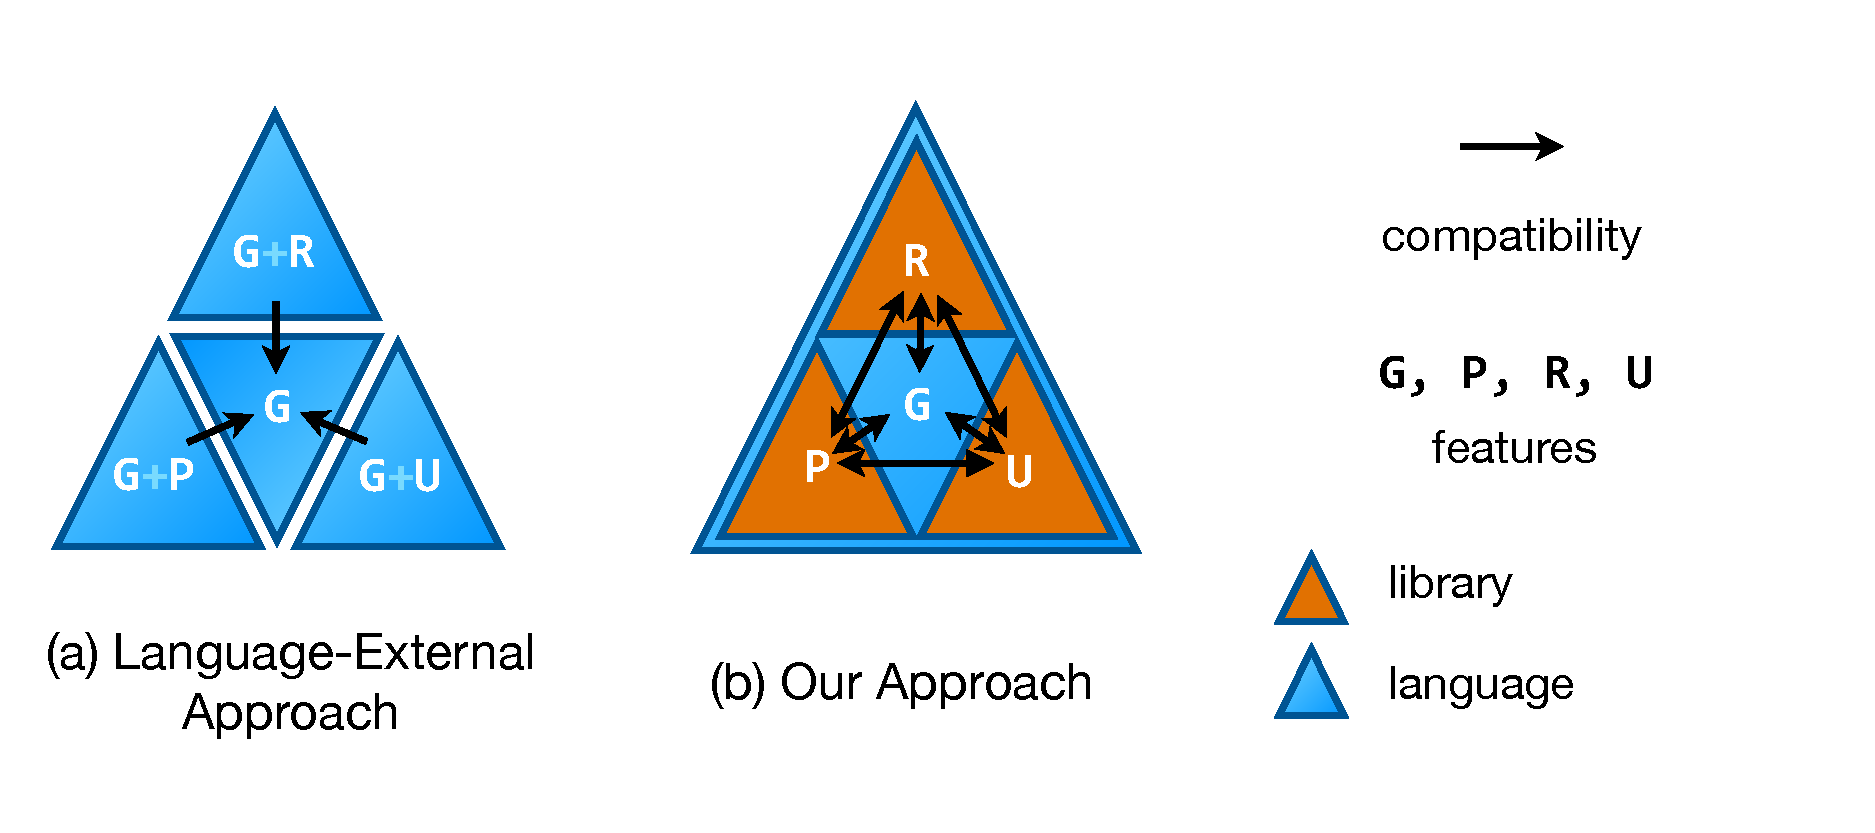
\includegraphics[scale=0.5]{approaches.pdf}
%\end{center}
%\vspace{-20px}
%\caption{\small (a) With a language-oriented approach, novel constructs are packaged into separate languages. Users can only safely and naturally call into languages consisting of common constructs (often only the common target language, such as C or Java bytecode). (b) With a language-internal extensibility approach, there is one system providing a common internal language, where additional primitive constructs that strictly strengthen its static guarantees or perform specialized code generation are specified and distributed within libraries. \label{approaches}}
%\end{figure*}

%As a result, domain-specific languages and new general-purpose abstractions alike have experienced relatively slow adoption in practice.
%
%Porting large codebases to new languages is difficult, and the dominant programming languages innovate slowly, so programming language.
%
%More specifically, such languages are neither \emph{internally extensible} because the language itself exposes only natural numbers and functions to its users, nor are they \emph{externally extensible} because no new behaviors can be added to the language's  implementation in a separate module from the one containing the initial implementation.

%This is the essence of a monolithic language implementation: it is impossible for anyone to modularly extend languages defined in this way. 

%\subsection{Theory}\label{atlam}
%%\begin{figure}
%%\begin{mathpar}
%%\inferrule{a}{b}
%%\end{mathpar}
%%\end{figure}
%In this section, we will describe a minimal calculus that captures our language-internal extensibility mechanism,  called \emph{active typechecking and translation (AT\&T)}. AT\&T allows developers to declare new primitive type families, associate operators with them, implement their static semantics in a functional style, and realize their dynamic semantics by simultaneously implementing a translation into a typed internal language. Note that this latter mechanism is closely related to how Standard ML was (re-)specified\todo{cite/read a bit about this/ask Bob/flesh this out}, but that we are fundamentally interested in extending language \emph{implementations}, not their  declarative specifications; proving the adequacy of such implementations against mechanized specifications, or extracting them directly from such specifications, will be investigated in future work.
%
%The AT\&T mechanism utilizes type-level computation of higher kind and integrates typed compilation techniques into the language to allow us to give strong metatheoretic guarantees,  and uses a mechanism notionally related to abstract types (such as those found in the ML module system) to guarantee that extensions cannot interfere with one another,  while remaining straightforward and expressive. In this section, we will develop a core calculus, called \atlam, which uses a minimal, uniform grammar for primitive operators. Then in Section \ref{ace}, we will show how to realize this minimal mechanism within a widely-used language with a more expressive grammar.
%
%AT\&T is general with respect to many choices about the type-level language, the typed internal language and syntax. Choices along these dimensions can affect both expressiveness and ease-of-use. We will begin in Sec. 2 by introducing a minimal system called $@\lambda$ (the ``actively-typed lambda calculus'') that distills the essence of the mechanism in a simply-typed, simply-kinded setting. This will allow us to fully and concisely formalize the language and compiler and give several key safety theorems. We will then continue in Sec. 3 by discussing variants of this mechanism based on other basic paradigms, considering dependently-typed functional languages and object-oriented languages, discussing trade-offs between expressivity and safety when doing so. We have developed a simple prototype called Ace and have used it to develop a number of full-scale language extensions as libraries. We will briefly discuss this language and these extensions in Sec. 4.

%We note at the outset that AT\&T focuses on extending the static semantics of languages with fixed, though flexible, syntax. Language-internal syntax extension mechanisms have been developed in the past (e.g. SugarJ \cite{sugarj}) but they have also suffered from safety problems because grammar composition is not always safe when done in an  unconstrained manner. Tyconstrained approaches that provide stronger safety guarantees have recently been outlined (e.g. Wyvern \cite{globaldsl13}) but we will leave integration of syntax extensions with semantic extensions as future work.


%\subsubsection{@$\lambda$: Conservatively Extending a Type System From Within}
%\begin{figure}[t]
%\small
%$$\begin{array}{rccl}	
%\textbf{programs} & \rho & ::= & \pfam{\familyDf}{\progsort}
%\\& &  \pipe & 
%%\pipe \pdef{t}{\kappa}{\tau}{\progsort} 
% e\\
%		&	\theta	&	::= &	\tops{op}{\kappaidx}{i}{a}{\taut{def}} \pipe 
%												\topp{\theta}{\theta}\\
%\\
%\textbf{external terms} 				&	e	&	::=	&	\evar{x} \pipe 
%%														\efix{x}{\tau}{e} \pipe 
%														\elam{\evar{x}}{\tau}{e} \pipe 
%														\eop{Tycon}{op}{
%															\tauidx
%														}{
%  												    		\splat{e}{1}{n}
%														} \\
%									& 		&		& 	\\
%
%
%\textbf{internal terms} 				& 	\iota	&	::=	&	\evar{x} \pipe 
%												\ifix{\evar{x}}{\sigma}{\iota} \pipe
%												\ilam{\evar{x}}{\sigma}{\iota} \pipe 
%												\iapp{\iota_{1}}{\iota_{2}} 
%\\\text{integers}&&\pipe&												
%												\iintlit \pipe \iop{\iota_{1}}{\iota_{2}} \pipe \iIfEq{\iota_{1}}{\iota_{2}}{\dint}{\iota_{3}}{\iota_{4}} \\
%\text{products}										& & \pipe & 
%												\iunit \pipe
%												\ipair{\iota_{1}}{\iota_{2}} \pipe 
%												\ifst{\iota} \pipe
%												\isnd{\iota} 
%\\\text{sums}&&\pipe&												
%												 \iinl{\sigma_2}{\iota_1} \pipe \iinr{\sigma_1}{\iota_2} \\&&\pipe& \icase{e}{x}{e_1}{x}{e_2} \\
%												
%%\text{deabstracted}& \iota & ::= & \mathcal{G}[\iota, \sigma]\\
%\textbf{internal types}			&	\sigma	&	::=	&    \darrow{\sigma_1}{\sigma_2} \pipe \dint \pipe \dunit \pipe \dpair{\sigma_1}{\sigma_2} \pipe \dsum{\sigma_1}{\sigma_2}  
%												
%\\
%\\
%							
%\hspace{-5pt}\textbf{type-level terms} 	& \tau 	& ::= 	& 	\tvar{t} \pipe 
%														\tlam{t}{\kappa}{\tau} \pipe 
%														\tapp{\tau_1}{\tau_2} \pipe \iintlit \pipe \iop{\tau_1}{\tau_2} \pipe \tlabel{label}
%\\\text{lists}&&\pipe&											
%														\tnil{\kappa} \pipe \tcons{\tau_1}{\tau_2} \pipe 
%									                     \tfold{\tau_1}{\tau_2}{h}{t}{r}{\tau_3}
%														\\
%												
%\text{products}	 			& 		& \pipe	& 	  \tunit \pipe 
%														\tpair{\tau_{1}}{\tau_{2}} \pipe 
%														\tfst{\tau} \pipe 
%														\tsnd{\tau} 
%														\\	
%\text{sums}									&       & \pipe & \tinl{\kappa_2}{\tau_1} \pipe \tinr{\kappa_1}{\tau_2} \\&&\pipe& \tsumcase{\tau}{t}{\tau_1}{t}{\tau_2} \\
%						\text{types} 						& 		& \pipe	& 	\ttypestd \\&&\pipe& \tfamcase{\tau}{Tycon}{x}{\tau_1}{\tau_2}\\
%\text{equality}  & & \pipe & 					\tifeq{\tau_{1}}{\tau_{2}}{\kappa}{\tau_{3}}{\tau_{4}} 
%														\\													%				& & \pipe & \tfamcase{\tau}{Fam}{x}{\tau_1}{\tau_2}\\
%																								
%\text{derivates} 				& 		 & 	\pipe	&	\tden{\tau_2}{\tau_1} \pipe \tden{\tau_2}{\tau_1}^{\checkmark} \pipe \ttypeof{\tau} \\% \tdencase{\tau}{x}{t}{\tau_1}{\tau_2}\\
% %& & \pipe & 
%%														\tdencase{\tau}{y}{x}{\tau_1}{\tau_2}
%%														 \\
%
%\text{translational IL}		&		&	\pipe	&	\titerm{\bar \iota} \pipe \titype{\bar \sigma} \\
%% &  & \pipe & \tvalof{\tau_1}{\tau_2} \pipe \iup{\tau} \\
%% 												\trepof{\tau} \pipe \dup{\tau}\\
%	& \bar{\iota} & ::= & x \pipe \ifix{x}{\bar \sigma}{\bar \iota} 
%	%\pipe \ilam{x}{\bar \sigma}{\bar \iota} \pipe \iapp{\bar \iota_1}{\bar \iota_2} 
%	\pipe \cdots \pipe \iup{\tau} \pipe \itransof{\tau} \\						
% & \bar{\sigma} & ::= & \darrow{\bar \sigma_1}{\bar \sigma_2} \pipe \cdots \pipe \dup{\tau} \pipe \trepof{\tau} \\
%%\text{abstracted} & \sabs & ::= & \darrow{\sabs_1}{\sabs_2} \pipe \cdots \pipe \sabsrep{\tau}
%											\\
%\textbf{kinds} 					& \kappa	&	::=	&	\karrow{\kappa_1}{\kappa_2} \pipe \kint \pipe
%											    \klabel \pipe
%											    \klist{\kappa} \pipe
%												\kunit \pipe 
%												\kpair{\kappa_{1}}{\kappa_{2}} \\
%												&&\pipe&
%												\ksum{\kappa_1}{\kappa_2} \pipe
%												\kTypeBlur \pipe \kDen \pipe 
%												\kIType								
%%\textbf{ops signature}			& \Theta	&	::=	&	\kOpEmpty \pipe \kOp{\Theta}{op}{\kappai}\\
%%											 							&		&		&	\\
%\end{array}$$
%\vspace{-10px}
%\caption{\small Syntax of Core \atlam. Here, $x$ ranges over external and internal language variables, $\tvar{t}$ ranges over type-level variables, $\fvar{Tycon}$ ranges over type constructor names, $\opvar{op}$ ranges over operator constructor names, $\iintlit$ ranges over integer literals, $\tlabel{label}$ ranges over label literals (see text) and $\oplus$ ranges over standard total binary operations (e.g. addition, comparison).
%\label{grammar}}
%\vspace{-5px}
%\end{figure}
%\begin{figure}[t]
%\small
%\begin{flalign}
%\label{natfam}&\family{Nat}{\kunit}{\\
%\label{z}&\quad\tops{z}{\kunit}{i}{a}{\tlam{i}{\kunit}{\tlam{a}{\klist{\kDen}}{
%	\tapp{\tapp{\tvar{arity0}}{\tvar{a}}}{\\&\quad\quad
%		\tden{\titerm{0}}{\ttype{Nat}{\tunit}}
%	}}}};\\
%\label{s}&\quad\tops{s}{\kunit}{i}{a}{\tlam{i}{\kunit}{\tlam{a}{\klist{\kDen}}{\tvar{arity1}~\tvar{a}~\tlam{d}{\kDen}{\\
%& \quad\quad \tvar{ifeq}~\ttypeof{\tvar{d}}~\ttype{Nat}{\tunit}\\
%& \quad\quad\quad \tden{\titerm{\itransof{\tvar{d}} + 1}}{\ttype{Nat}{\tunit}}
%	}}}};\\
%\label{rec}&\quad\tops{rec}{\kunit}{i}{args}{\tlam{i}{\kunit}{\tlam{a}{\klist{\kDen}}{\tvar{arity3}~\tvar{a}~\tlam{d1}{\kDen}{\tlam{d2}{\kDen}{\tlam{d3}{\kDen}{\\
%&\quad\quad \tvar{ifeq}~\ttypeof{\tvar{d1}}~\ttype{Nat}{\tunit}\\
%&\quad\quad {\sf let}~\tvar{t2} = \ttypeof{\tvar{d2}}~{\sf in}\\
%&\quad\quad \tvar{ifeq}~\ttypeof{\tvar{d3}}~\ttype{Arrow}{(\ttype{Nat}{\tunit}, \ttype{Arrow}{(\tvar{t2}, \tvar{t2})})}\\
%&\quad\quad\quad \tden{\titerm{\iapp{(\ifix{f}{\darrow{\dint}{\trepof{\tvar{t2}}}}{\ilam{x}{\dint}{\\
%		\label{lastop}&\quad\quad\quad\quad\quad \iIfEq{x}{0}{\dint}{\itransof{\tvar{d2}}}{
%		%\\&\quad\quad\quad\quad\quad\quad
%		\iapp{\iapp{\itransof{\tvar{d3}}}{(x-1)}}{(\iapp{f}{(x-1)})}}}}\\
%		&\quad\quad\quad\quad)}{\itransof{\tvar{d1}}}}}{\tvar{t2}}
%}}}
%}}}
%\\
%&}{XXX}{i}{\tlam{i}{\kunit}{\titype{\dint}}};\\
%\label{nattype}&{\sf let}~\tvar{nat} = \ttype{Nat}{\tunit}~{\sf in}\\
%& \elet{two}{\eop{Nat}{s}{\tunit}{\eop{Nat}{s}{\tunit}{\eop{Nat}{z}{\tunit}{}}}}{\\
%& \elet{plus}{
%	\elam{x}{\tvar{nat}}{
%		\elam{y}{\tvar{nat}}{
%			\\&\quad \eop{Nat}{rec}{\tunit}{x; y; \elam{p}{\tvar{nat}}{\elam{r}{\tvar{nat}}{
%				\eop{Nat}{s}{\tunit}{r}
%			}}}
%		}
%	}
%}{
%& \\
%& \eop{Arrow}{ap}{\tunit}{plus; \eop{Arrow}{ap}{\tunit}{two; two}}
%}}
%%{\\&\elet{two}{\tvar{nat}}{\eop{Nat}{s}{\tunit}{\eop{Nat}{s}{\tunit}{\eop{Nat}{z}{\tunit}{ }}}}{\eapp{\eapp{plus}{two}}{two}}}
%%}
%%\elam{x}{\tvar{nat}}{\elam{y}{\tvar{nat}}{\\
%	%&\quad \eop{Nat}{rec}{\tunit}{x; y; \elam{p}{\tvar{nat}}{\elam{r}{\tvar{nat}}{
%	%\eop{Nat}{s}{\tunit}{r}
%	%}}}}
%\end{flalign}
%%\vspace{-15px}
%\caption{\small An program that defines and uses an embedding of G\"odel's $\mathbf{T}$ into \atlam\, to define $plus$ and $two$ and calculate $plus~two~two$. Type constructors (line 1) and types (line 15) are discussed in Sec. \ref{types}. Schemas (line 1) and operator constructors (lines 2-14, used on lines 16-19) are discussed starting in Sec. \ref{opcons}. We use \textsf{let} to bind both external and type-level variables as needed for clarity of presentation. We will discuss further syntactic issues later.}
%\label{nat}
%\vspace{-10pt}
%\end{figure}
%\begin{figure}[t]
%\small
%\begin{flalign}
%\label{natfam}&\family{Nat}{\kunit}{\\
%\label{z}&\quad\tops{z}{\kunit}{i}{a}{\tlam{idx}{\kunit}{\tlam{args}{\klist{\kDen}}{
%	\tapp{\tapp{\tvar{if\_empty}}{\tvar{args}}}{
%		\tden{\titerm{0}}{\ttype{Nat}{\tunit}}
%	}}}};\\
%\label{s}&\quad\tops{s}{\kunit}{i}{a}{\tlam{idx}{\kunit}{\tlam{args}{\klist{\kDen}}{\\
%& \quad\quad
%	\tapp{
%		\tapp{\tvar{pop\_final}}{\tvar{args}}}{\tlam{x}{\kITerm}{\tlam{t}{\kTypeBlur}{
%			\\
%			&\quad\quad\tapp{\tapp{\tapp{\tvar{check\_type}}{\tvar{t}}}{\ttype{Nat}{\tunit}}}{
%				\tden{\titerm{\iup{\tvar{x}}+1}}{\ttype{Nat}{\tunit}}
%			}
%		}}
%		}
%	}}};\\
%\label{rec}&\quad\tops{rec}{\kunit}{i}{args}{\tlam{idx}{\kunit}{\tlam{args}{\klist{\kDen}}{\\
%& \quad\quad
%	\tapp{\tapp{\tvar{pop}}{\tvar{args}}}{\tlam{x1}{\kITerm}{\tlam{t1}{\kTypeBlur}{\tlam{args}{\klist{\kDen}}{\\
%	&\quad\quad\tapp{\tapp{\tvar{pop}}{\tvar{args}}}{\tlam{x2}{\kITerm}{\tlam{t2}{\kTypeBlur}{\tlam{args}{\klist{\kDen}}{\\
%	&\quad\quad \tapp{\tapp{\tvar{pop\_final}}{\tvar{args}}}{\tlam{x3}{\kITerm}{\tlam{t3}{\kTypeBlur}{\\
%	&\quad\quad \tapp{\tapp{\tapp{\tvar{check\_type}}{\tvar{t1}}}{\ttype{Nat}{\tunit}}}{(\\
%	&\quad\quad \tapp{\tapp{\tapp{\tvar{check\_type}}{\tvar{t3}}}{\ttype{Arrow}{(\ttype{Nat}{\tunit},\ttype{Arrow}{(\tvar{t2},\tvar{t2})})}}}{\\
%		\label{fix}&\quad\quad \tden{\titerm{\iapp{(\ifix{f}{\darrow{\dint}{\trepof{\tvar{t2}}}}{\ilam{x}{\dint}{\\
%		\label{lastop}&\quad\quad\quad \iIfEq{x}{0}{\dint}{\iup{\tvar{x2}}}{\iapp{\iapp{\iup{\tvar{x3}}}{(x-1)}}{(\iapp{f}{(x-1)})}}}})}{\iup{\tvar{x1}}}}}{\tvar{t2}}
%	)}}
%	}}}}}}}}}}}}}}
%\\
%&}{XXX}{i}{\tlam{idx}{\kunit}{\titype{\dint}}};\\
%\label{nattype}&\etdef{nat}{\kTypeBlur}{\ttype{Nat}{\tunit}}{\\
%& \elet{plus}{\ttype{Arrow}{(\tvar{nat}, \ttype{Arrow}{(\tvar{nat}, \tvar{nat})})}}{
%	\elam{x}{\tvar{nat}}{
%		\elam{y}{\tvar{nat}}{
%			\\&\quad \eop{Nat}{rec}{\tunit}{x; y; \elam{p}{\tvar{nat}}{\elam{r}{\tvar{nat}}{
%				\eop{Nat}{s}{\tunit}{r}
%			}}}
%		}
%	}
%}{\\
%& \elet{two}{\tvar{nat}}{\eop{Nat}{s}{\tunit}{\eop{Nat}{s}{\tunit}{\eop{Nat}{z}{\tunit}{}}}}{\\
%& \eop{Arrow}{ap}{\tunit}{plus; \eop{Arrow}{ap}{\tunit}{two; two}}
%}}}
%%{\\&\elet{two}{\tvar{nat}}{\eop{Nat}{s}{\tunit}{\eop{Nat}{s}{\tunit}{\eop{Nat}{z}{\tunit}{ }}}}{\eapp{\eapp{plus}{two}}{two}}}
%%}
%%\elam{x}{\tvar{nat}}{\elam{y}{\tvar{nat}}{\\
%	%&\quad \eop{Nat}{rec}{\tunit}{x; y; \elam{p}{\tvar{nat}}{\elam{r}{\tvar{nat}}{
%	%\eop{Nat}{s}{\tunit}{r}
%	%}}}}
%\end{flalign}
%\vspace{-15px}
%\caption{\small G\"odel's $\mathbf{T}$ in \atlam, used to calculate 2+2. The simple helper functions $\tvar{if\_empty}$, $\tvar{pop}$, $\tvar{pop\_final}$, $\tvar{check\_type}$ all have return kind $\ksum{\kDen}{\kunit}$ (see text). Their definitions can be found in the appendix. We use \textsf{let} to bind both external and type-level variables for clarity of presentation; these can be eliminated by manually performing the indicated substitutions (or added to the semantics).}
%\label{nat}
%\end{figure}
%
%\begin{figure}[t]
%\begin{lstlisting}
%tycon Nat of 1 with  
%    schema $\lambda$idx:1.$\blacktriangledown$($\mathbb{Z}$) 
%    opcon Z of 1 ($\lambda$idx:1.$\lambda$args:list[Elab].is_empty args $\llbracket$$\triangledown$(0) as Nat[()]$\rrbracket$)
%    opcon S of 1 ($\lambda$idx:1.$\lambda$args:list[Elab].pop_final args $\lambda$x:ITm.$\lambda$ty:$\star$. 
%      checktype ty Nat[()] $\llbracket$$\triangledown$($\vartriangle$(x)+1) as Nat[()]$\rrbracket$)
%    opcon Rec of 1 ($\lambda$idx:1.$\lambda$args:list[Elab].
%      pop args $\lambda$x1:ITm.$\lambda$ty1:$\star$.$\lambda$args':list[Elab].
%      pop args' $\lambda$x2:ITm.$\lambda$ty2:$\star$.$\lambda$args'':list[Elab].
%      pop_final args'' $\lambda$x3:ITm.$\lambda$ty3:$\star$.
%      check_type t1 Nat[()] (
%      check_type t3 Arrow[(Nat[()], Arrow[(t2, t2)])] 
%      	$\llbracket$$\triangledown$((fix f:$\mathbb{Z} \rightarrow$ rep(t2) is $\lambda$x:$\mathbb{Z}$.
%	        if x = 0 then $\vartriangle$(x2) else $\vartriangle$(x3) (x - 1) (f (x - 1))) $\vartriangle$(x1)) as t2$\rrbracket$))
%end
%\end{lstlisting}
%\caption{An implementation of primitive natural numbers as internal integers in @$\lambda$.}
%\label{nat-atlam}
%\end{figure}
%In this section, we will develop an ``actively typed'' version of the simply-typed lambda calculus with simply-kinded type-level computation called @$\lambda$. More specifically, the level of types, $\tau$, will itself form a simply-typed lambda calculus. \emph{Kinds} classify type-level terms in the same way that types conventionally classify expressions. Types become just one kind  of type-level value (which we will write $\kTypeBlur$, though it is also variously written $\star$, \verb|T| and \verb|Type| in various settings). Rather than there being a fixed set of type and operator constructors, we allow the programmer to declare new  constructors, and give their static and dynamic semantics by writing type-level functions. The kind system combined with techniques borrowed from the typed compilation literature and a form of type abstraction will allow us to prove strong type safety, decidability and conservativity theorems.
%
%The syntax of Core @$\lambda$ is given in Fig. \ref{grammar}. An example of a program defining type and operator constructors that can be used to construct an active embedding of G\"odel's \textbf{T} into @$\lambda$ is given in Fig. \ref{nat}. We will discuss its semantics and how precisely the embedding, seen being used starting on line 15 to ultimately compute the sum of two and two, works as we go on. Natural numbers can, of course, be isomorphically embedded in existing languages, with a similar usage and asymptotic performance profile (up to function call overhead as an abstract type, for example). We will provide more sophisticated examples where this is less feasible later on (and note that type abstraction is an orthogonal mechanism).
%%a type constructor declaration, $\fvar{Nat}$, indexed trivially, together with three operator constructors, also all indexed trivially, that implement the standard introductory forms for natural numbers as well as the recursor operator (as in G\"odel's T \cite{pfpl}). Following the type constructor declaration, we apply $\fvar{Nat}$ with the trivial index, $\tunit$, to form the type $\tvar{nat}$. Finally, we write an external term that uses the operators associated with $\fvar{nat}$ and the built-in constructor $\fvar{Parr}$, governing partial functions, to define an addition function and compute the addition of the natural numbers  two and two. We will introduce a more convenient concrete syntax in later portions of this thesis; for now we will restrict ourselves to the abstract syntax so that this example can directly aid in understanding the semantics.
%
%\subsection{Overview}\label{programs}
%
%A \emph{program}, $\rho$, consists of a series of constructor declarations (lines 1-14 of Figure \ref{nat}) followed by an external term, $e$ (lines 15-19). The syntax for external terms (Figure \ref{grammar}) contains three forms: variables, $\lambda$ terms, and a form for invoking user-defined operators, which we will discuss below. Compiling a program consists of first \emph{kind checking} it, then typechecking the external term and simultaneously {translating} it to a term, $\iota$, in the {typed internal language}. 
%%These correspond to the premises of the \emph{central compilation judgement} $\pkcompiles{\rho}{\iota}$:
%%\[
%%\inferrule[p-compiles]{
%%	\emptyset \vdash_{\fvalCtx_0} \rho\\
%%%	\progOK{\emptyset}{\fvalCtx_0}{\rho}\\
%%	\pcompiles{\fvalCtx_0}{\rho}{\iota}
%%}{\pkcompiles{\rho}{\iota}}
%%\]
%%This anchors our exposition; we will describe how it is derived (i.e. how to write a compiler for @$\lambda$) in the following sections. 
%The key judgement is the \emph{active typing judgement}  (Fig. \ref{att}, which we describe starting in Sec. \ref{opcons}). It relates an external term, $e$, to a {type}, $\tau$, called its \emph{type assignment}, and an internal term, $\iota$, called its \emph{translation}, under \emph{typing context} $\Gamma$ and \emph{constructor context} $\Phi$: 
%\[\ecompilesX{e}{\tau}{\iota}\]
%
%The typing context, $\Gamma$, maps variables to types in essentially the conventional way (\cite{pfpl} contains the necessary background for this thesis). The constructor context, $\Phi$, tracks user-defined type and operator constructors. % Weakening and exchange of the constructor context closely related to the issue of conservativity that we will return to. Each constructor is identified by name, so there is no analog to contraction.
%
%The dynamic behavior of an external term is determined entirely by its translation to the internal language, which has a conventional operational semantics. This form of semantics can be seen as lifting into the language specification the first stage of a type-directed compiler like the TIL compiler for Standard ML \cite{tarditi+:til-OLD} and has some parallels to the Harper-Stone semantics for Standard ML, where external terms were also given meaning by elaboration from the EL to an IL \cite{Harper00atype-theoretic}. %
%
%In @$\lambda$, the internal language (IL) provides partial functions (via the generic fixpoint operator of Plotkin's PCF), simple product and sum types and a base type of integers (to make our example interesting and as a nod toward efficiency on contemporary machines). In practice, the internal language could be any typed  language with a specification for which type safety and decidability of typechecking have been satisfyingly determined. The internal type system serves as a ``floor'': guarantees that must hold for terms of any type (e.g. that out-of-bounds access to memory never occurs) must be maintained by the internal type system. User-defined constructors can enforce invariants stronger than those the internal type system maintains at particular types, however. Performance is also ultimately limited by the internal language and downstream compilation stages that we do not here consider (safe compiler extension has been discussed in previous work, e.g. \cite{conf/pldi/TatlockL10}).
%
%
%\subsection{Type Constructors and Types}\label{types}
%In most languages, types are formed by applying one of a collection of \emph{type constructors} to zero or more \emph{indices}. In @$\lambda$, the situation is notionally similar. User-defined type constructors can be declared at the top of a program (or lifted to the top, in practice) using \textsf{tycon}. Each constructor in the program must have a unique name, written e.g. \fvar{Nat}.\footnote{We assume naming conflicts can be avoided by some extrinsic mechanism.} A type constructor must also declare an \emph{index kind}, $\kappaidx$. A type is introduced by applying a type constructor to an index of this kind, written $\ttype{Tycon}{\tauidx}$.  For example, the type of natural numbers is indexed trivially, so it is written $\ttype{Nat}{\tunit}$ (similar to our abstract syntax for G\"odel's \textbf{T} in Fig. \ref{natfrag}). We abbreviate it on line 15.
%
%@$\lambda$ supports, and makes extensive use of, simply-kinded type-level computation. Specifically, type-level terms, $\tau$, themselves form a typed lambda calculus. The classifiers of type-level terms are called \emph{kinds}, $\kappa$, to distinguish them from  \emph{types}. The kinding rules are specified in the paper draft (see below). Types are  type-level values of kind $\kTypeBlur$, introduced as just described. The kind $\kTypeBlur$ also has an elimination form, $\tfamcase{\tau}{Tycon}{x}{\tau_1}{\tau_2}$, allowing the extraction of a type index by case analysis against a contextually-available type constructor. To a first approximation, one might think of type constructors as constructors of a built-in open datatype, $\kTypeBlur$, at the type-level. Like open datatypes, there is no notion of exhaustiveness so the default case is required for totality.
%%We will write the kind of types as $\kTypeBlur$, though it is also written $\star$ or \verb|Type| in various similarly structured languages (see Sec. \ref{related-work}). 
%% Rather than there being a fixed set of type constructors, we allow the programmer to declare new type  constructors, and give the static and dynamic semantics of their associated operators, by writing type-level functions. In the semantics for this calculus, our kind system combined with techniques borrowed from the typed compilation literature and a form of type abstraction allow us to prove strong type safety, decidability and conservativity theorems.
%
%
% To permit the embedding of interesting type systems, the type-level language includes several kinds other than $\kTypeBlur$. We lift several  standard functional fragments to the type level: unit ($\kunit$), binary products ($\kpair{\kappa_1}{\kappa_2}$), binary sums ($\ksum{\kappa_1}{\kappa_2}$), lists ($\klist{\kappa}$) and integers ($\dint$). We also include labels ($\klabel$), written in a slanted font, e.g. $\tlabel{myLabel}$, which are string-like values that only support comparison and play a distinguished role in the expanded syntax, as we will later discuss. Our first example, $\fvar{Nat}$, is indexed trivially, i.e. by unit kind, $\kunit$, so there is only one natural number type, $\ttype{Nat}{\tunit}$, but we will show examples of type constructors that are indexed in more interesting ways in later portions of this work. For example, $\fvar{LabeledTuple}$ has index kind $\klist{\kpair{\klabel}{\kTypeBlur}}$. The type constructor $\fvar{Arrow}$ is included in the initial constructor context, $\fvalCtx_0$, shown in the paper draft, and has index kind $\kpair{\kTypeBlur}{\kTypeBlur}$. We will return to arrow types in the next subsection.
% 
% Type constructors are not first-class; they do not themselves have arrow kind as in some kind systems (e.g.  \cite{watkins2008specifying}; Ch. 22 of \emph{PFPL} describes a related system \cite{pfpl}). The type-level language does, however, include total functions of arrow kind, written $\karrow{\kappa_1}{\kappa_2}$. Type constructor application can be wrapped in a type-level function to emulate a first-class or uncurried version of a type constructor for convenience (indeed, such a wrapper could be generated automatically, though we do not do so). 
%
%Two type-level terms of kind $\kTypeBlur$ are equivalent if they apply the same constructor, identified by name, to equivalent indices. Going further, we ensure that deciding type equivalence requires only checking for syntactic equality after normalization by imposing the restriction that equivalence at a type constructor's index kind must be decidable in this way. Our treatment of equivalence in the type-level language is thus quite similar to the treatment of term-level equality using ``equality types'' in a language like Standard ML. A kind $\kappa$ is an  \emph{equality kind} if $\kEq{\kappa}$ can be derived (see draft). Conditional branching on the basis of equality at an equality kind can be performed in the type-level language (e.g. in \tvar{ifeq}, Fig. \ref{helpers}, discussed below). Equivalence at arrow kind is not decidable by our criteria, so type-level functions cannot appear within type indices. This also prevents general recursion from arising at the type level. Without this restriction, a type-level function taking a type as an argument could ``smuggle in'' a self reference as a type index, extracting it via case analysis (continuing our analogy to open datatypes, this is closely related to the positivity condition for inductive datatypes in total functional languages like Coq).% as maintaining the metatheoretic guarantee that typing respects type equivalence would impose a substantial burden in such a setting.% (a na\"ive approach to this would impose non-trivial extrinsic proof obligations onto extension developers that, unlike in others in this thesis, could threaten type safety).
%
%Every type constructor also defines a \emph{schema}, a type-level function that associates with every type an internal \emph{representation type}. We will return to this in Sec. \ref{repcon}. 
%
%\subsection{Operators and Operator Constructors}\label{opcons}
%
%User-defined operator constructors are declared using \textsf{opcon}.  For reasons that we will discuss, our calculus associates every operator  constructor with a type constructor. The \emph{fully-qualified name} of every operator constructor, e.g. $\fvar{Nat}.\opvar{z}$, must be unique. Operator constructors, like type constructors, declare an index kind, $\kappaidx$. In our first example, all the operator constructors are indexed trivially (by index kind $\kunit$), but other examples use more interesting indices. For example, in SML, the projection operator \verb|#3| can be applied to an $n$-tuple, $e$, iff $n \geq 3$. Note that it thus cannot be a function with a standard arrow type. Notionally, \verb|#| is an operator constructor and \verb|3| is its index. In an active embedding of $n$-tuples into @$\lambda$, this would be written $\eop{Tuple}{prj}{3}{e}$ (we will nearly recover ML's syntax later). $\fvar{LabeledTuple}.\opvar{prj}$ is the operator constructor used to access a field of a labeled tuple, so it has index kind $\klabel$. An operator itself is, notionally, selected by indexing an operator constructor, e.g. $\fvar{Nat}.\opvar{s}\langle \tunit \rangle$, but technically neither operator constructors nor operators are first-class at any level (additional machinery would be needed, e.g. an \textsf{Op} kind, but this is not fundamental to our calculus). 
%Instead, in the external language, an operator constructor is applied by simultaneously providing an index and  $n \geq 0$ \emph{arguments}, written $\eop{Tycon}{op}{\tauidx}{\splat{e}{1}{n}}$\footnote{It may be helpful to distinguish between type/operator constructors and \emph{term formers}. There are term formers at all levels in the calculus. For example, operator constructor application and $\lambda$ are  external term formers, and type constructor application is a type-level term former. We might write these following Harper's conventions for abstract syntax to highlight this distinction \cite{pfpl}: $\mathtt{lam}[\tau](x.e)$, $\mathtt{ocapp}[\fvar{Tycon}, \opvar{op}, \tauidx](\splat{e}{1}{n})$ and $\texttt{tcapp}[\fvar{Tycon}](\tau)$.}. For example, on line 18 of Fig. \ref{nat}, we see the operator constructors $\fvar{Nat}.\opvar{z}$ and $\fvar{Nat}.\opvar{s}$ being applied to compute $two$. %\footnote{Although our focus here is entirely on semantics, a brief note on syntax: in the expanded syntax, the trivial indices and empty argument lists can be omitted, so we could write \texttt{Nat.s(Nat.s(Nat.z))}. With the ability to ``open'' a type's operators into the context, we could shorten this still to \texttt{s(s(z))}. Alternatively, with the ability to define a TSL in a manner similar to that in Sec. \ref{aparsing}, we might instead just write \texttt{2}.}
%
%\subsection{Operator Definitions and Derivates}
%The expressive and metatheoretic power of the calculus arises from how the rules for the active typing judgement handle this  operator constructor application form. Rather than fixing the specification of a finite collection of operator constructors and tasking the \emph{compiler} with deciding a typing derivation on its basis, the specification instead tasks the \emph{operator constructor's definition}: {a type-level function that must decide the type assignment and the translation on the basis of the index and arguments, or decide that this is not possible}. An operator constructor with index kind $\kappaidx$ must have a definition of kind \[\kappaidx \rightarrow \klist{\kDen} \rightarrow (\kDen + \kunit)\] 
%As this suggests, the active typing judgement  will provide the operator index and a list of {recursively determined \emph{derivates}}, which have kind $\kDen$, for the arguments and ask the definition to return a value of ``option kind'', $\ksum{\kDen}{\kunit}$, where the trivial case indicates that a derivate cannot be constructed due to an invalid index, an incorrect number of arguments or an argument of an invalid type.\footnote{In practice, we would require operator constructor providers to report information about the precise location of the error (e.g. which argument was of incorrect type) and provide an appropriate error message and other metadata, but we omit this in the semantics.}
%\begin{figure}[t]
%\small
%\[
%\begin{array}{rcl}
%\tvar{failure} & := & \tinr{\kDen}{\tunit}\\
%\tvar{ok} & := & (\tlam{d}{\kDen}{\tinl{\kunit}{\tvar{d}}})\\
%\tvar{ifeq} & := & (\tlam{t1}{\kTypeBlur}{\tlam{t2}{\kTypeBlur}{\tlam{d}{\kDen}{
%	\\& & \quad \tifeq{\tvar{t1}}{\tvar{t2}}{\kTypeBlur}{\tvar{ok}~\tvar{d}}{\tvar{failure}}\\
%\tvar{arity0} & := & (\tlam{a}{\klist{\kDen}}{\tlam{d}{(\ksum{\kDen}{\kunit})}{\tfold{\tvar{a}}{\tvar{d}}{\_}{\_}{\_}{\tvar{failure}}}})\\
%\tvar{arity1} & := & (\tlam{a}{\klist{\kDen}}{\tlam{k}{\karrow{\kDen}{(\ksum{\kDen}{\kunit})}}{
%	\\ & & \quad \tfold{\tvar{a}}{\tvar{tyerr}}{h}{t}{\_}{
% \tvar{arity0}~\tvar{t}~(\tvar{k}~\tvar{h})}}})\\
%\tvar{arity2} & := & (\tlam{a}{\klist{\kDen}}{\tlam{k}{\karrow{\kDen}{\karrow{\kDen}{(\ksum{\kDen}{\kunit})}}}{
%	\\ & & \quad \tfold{\tvar{a}}{\tvar{tyerr}}{h}{t}{\_}{
% \tvar{arity1}~\tvar{t}~(\tvar{k}~\tvar{h})}}})\\
% \tvar{arity3} & := & (\tlam{a}{\klist{\kDen}}{\tlam{k}{\karrow{\kDen}{\karrow{\kDen}{\karrow{\kDen}{(\ksum{\kDen}{\kunit})}}}}{
%	\\ & & \quad \tfold{\tvar{a}}{\tvar{tyerr}}{h}{t}{\_}{
% \tvar{arity2}~\tvar{t}~(\tvar{k}~\tvar{h})}}})
%}}}
%\end{array}
%\]
%\caption{\small Useful (type-level) functions for writing operator definitions.}
%%\vspace{-pt}
%\label{helpers}
%\end{figure}
%
%A \emph{derivate} is introduced in operator definitions by the form $\tden{\tau_2}{\tau_1}$, where $\tau_1$ is a type assignment, of kind $\kTypeBlur$, and $\tau_2$ is a translation, of kind $\kITerm$. This kind has introductory form $\titerm{\ibar}$, where $\ibar$ is a translational internal term, and no elimination form. The syntax for translational internal terms mirrors that of internal terms, $\iota$, adding two additional forms:
%\begin{enumerate}
%\item $\iup{\tau}$ splices in another translational internal term $\tau$
%\item $\itransof{\tau}$ refers to the translation of the derivate $\tau$
%\end{enumerate}
%%The paper draft shows the kinding rules for derivates and translational internal terms (we will discuss checked derivates shortly; they are only used internally by the semantics). 
%
% Note that there is no elimination form for directly extracting a translation from a derivate, so the second form is not subsumed by the first. This is the only way to compose derivates from other derivates. We will see why shortly. Only the type assignment can be extracted directly from a derivate, using $\ttypeof{\tau}$.
%
%Let us return to Fig. \ref{nat} to build intuition. 
%The definition of $\fvar{Nat}.\opvar{z}$ in Fig. \ref{nat} is quite simple: it returns the derivate $\tden{\titerm{0}}{\ttype{Nat}{\tunit}}$ if no arguments were provided, and indicates an error otherwise. This is done by calling a simple helper function, $\tvar{arity0}$, seen in Fig. \ref{helpers}. The definition of $\fvar{Nat}.\opvar{s}$ is only slightly more complex, because it requires inspecting a single argument. The helper function $\tvar{arity1}$ checks the arity of the argument list. If it is correct, it passes the single derivate to the shown continuation, returning the error case otherwise (which we give a more descriptive name, $\tvar{failure}$). The continuation we provided checks that the type of the argument is $\ttype{Nat}{\tunit}$ using a similar helper function, $\tvar{ifeq}$. If so, it constructs the derivate $\tden{\titerm{\itransof{\tvar{d}}+1}}{\ttype{Nat}{\tunit}}$ and $\tvar{ifeq}$ wraps it with $\tvar{ok}$. %These helper functions are shown in Fig. \ref{helpers}.% We will return to the recursor shortly.
%
%Recalling the active typing judgement mentioned earlier, these two operator definitions make the following rules admissible in a constructor context, let us call it $\fvalCtx_{\mathbf{T}}$, that extends the initial constructor context (defining only arrow types) with the constructors seen in  Fig. \ref{nat} (and any typing context valid under that constructor context):
%\newcommand{\fvalT}{\fvalCtx_{\mathbf{T}}}
%\begin{mathpar}
%\inferrule[gt-z]{ }{
%	\ecompiles{\Gamma}{\fvalT}{\eop{Nat}{z}{\tunit}{}}{\ttype{Nat}{\tunit}}{0}
%}
%
%\inferrule[gt-s]{
%	\ecompiles{\Gamma}{\fvalT}{e}{\ttype{Nat}{\tunit}}{\iota}
%}{
%	\ecompiles{\Gamma}{\fvalT}{\eop{Nat}{s}{\tunit}{e}}{\ttype{Nat}{\tunit}}{\iota + 1}
%}
%\end{mathpar}
%
%It can easily be seen that this is an isomorphic embedding of the introductory forms of that $\mathtt{nat}$ fragment of G\"odel's $\mathbf{T}$ (see Fig. \ref{natfrag}). If we keep the constructor context fixed, we would be able to prove this inductively, in fundamentally the same way that one would prove a compiler from $\mathbf{T}$ to the internal language correct. We will provide the details later. %The rules by which these are derived are given in the paper draft. We will discuss how they work informally below.
%
%% Figure \ref{att} shows how $\fvalCtx_{\mathbf{T}}$ would be built up and how these conclusions could be derived. The active typing judgement simply defers to the \emph{checked active typing judgement} (Fig. \ref{absatt}) to first produce a type assignment and a translational internal term, called the \emph{abstract translation}. It then \emph{deabstracts} the abstract translation to produce a type assignment and translation (Fig. \ref{deabstraction}). 
%% 
%% The rule \textsc{att-op} shows how operator constructor definitions are invoked. First, type assignments  and translational internal terms are recursively derived. Then, the operator constructor definition, $\taudef$ is extracted from the constructor context and applied to the index, $\tauidx$, and a list of \emph{checked derivates} constructed from the derivations produced in the first step. If this produces a derivate, $\tauD$, via the left case of the sum, then it is itself, finally, \emph{checked} to produce a type assignment, $\tau$, and translational internal term, $\ibar$. 
%% 
%%The normalization rules for type-level terms are shown in Fig. \ref{tleval} and are rather uninteresting. We will discuss their metatheoretic properties in Sec. \ref{theory}.
%% 
%% Derivate checking, shown in Fig. \ref{ait}, is described in the next two subsections. 
%% Note that derivate checks are still static checks; they do not change the translation. Derivate checking is sufficient to guarantee type safety and preclude interfere issues between extensions, as we will describe, because taking a path through an operator constructor definition that produces a problematic derivate will fail. If providers do not want to burden clients with this variety of error, which would require them to debug the constructor definition itself, we will discuss how constructor correctness could be verified mechanically by strengthening the kind system in Sec. \ref{limitations}. %We will discuss how to prove that an extension  operator definition could be \emph{proven} to not produce such derivates (so that users only ever face type errors arising from their own code, not also extension correctness issues) in Sec. \ref{limitations}. The checks are sophisticated enough that they cannot be eliminated by a simple kind system.  
%
%%$\tvar{pop\_final} : \karrow{\karrow{\klist{\kDen}}{(\karrow{\kTypeBlur}{\karrow{\kITerm}{(\ksum{\kDen}{\kunit})})}}}{(\ksum{\kDen}{\kunit})}$ ``pops'' a derivate from the head of the list and, if no other arguments remain, passes its translation and type to the ``continuation'', returning the error case otherwise. The continuation checks if the argument type is equal to $\ttype{Nat}{\tunit}$ using $\tvar{check\_type} : \karrow{\kTypeBlur}{\karrow{\kTypeBlur}{\karrow{\kDen}{(\ksum{\kDen}{\kunit})}}}$, which operates similarly. If these arity and type checks succeed, the resulting derivate is composed by adding one to the translation of the argument, passed into the continuation as $\tvar{x}$ in our example, and pairing it with the natural number type: $\tden{\titerm{\iup{\tvar{x}} + 1}}{\ttype{Nat}{\tunit}}$. We will return to the definition of $\fvar{Nat}.\opvar{rec}$ after in the next subsection.
%
%%We leave adding the ability to declare and manipulate new contexts as future work.
%
%%\begin{figure}[t]
%%\small
%%\[
%%\begin{array}{rcl}
%%\Phi_0 & := & \emptyset, \fval{Arrow}{\kpair{\kTypeBlur}{\kTypeBlur}}{\tau_0}{\theta_0}\\
%%\tau_0 & := & \tlam{i}{\kpair{\kTypeBlur}{\kTypeBlur}}{\titype{\darrow{\trepof{\tfst{\tvar{i}}}}{\trepof{\tsnd{\tvar{i}}}}}}\\
%%\theta_0 & := & \tops{ap}{\kunit}{i}{a}{
%%	\tlam{i}{\kunit}{\tlam{a}{\klist{\kDen}}{
%%		\tvar{arity2}~\tvar{a}~\tlam{d1}{\kDen}{\tlam{d2}{\kDen}{
%%		\\& & \quad \tfamcase{\ttypeof{\tvar{d1}}}{Arrow}{x}{
%%		\\& & \quad\quad \tvar{ifeq}~\tfst{\tvar{x}}~\ttypeof{\tvar{d2}}
%%		\\& & \quad\quad\quad \tden{\itransof{\tvar{d1}}~\itransof{\tvar{d2}}}{\tsnd{\tvar{x}}}
%%		\\& & \quad\hspace{-3px}}{\tvar{tyerr}}
%%		}}
%%	}}
%%}
%%\end{array}
%%\]
%%\caption{\small The initial constructor context, $\fvalCtx_0$, defines the $\fvar{Arrow}$ type constructor. The introductory form, $\elam{x}{\tau}{e}$, is built into the language but the elimination form goes through the operator constructor $\fvar{Arrow}.\opvar{ap}$.}
%%\label{arrow}
%%\end{figure}
%%

%\subsection{Parametricity Implies Conservativity}
%\begin{figure}[t]
%\small
%$\fbox{\inferrule{}{\pcompilesX{\rho}}}$
%\begin{mathpar}
%\inferrule[att-tycon]{
%	\pcompiles{\fvalCtxX{\fvalDf}}{\rho}{\iota}
%}{
%	\pcompilesX{\pfam{\familyDf}{\rho}}
%}
%%
%%\inferrule[att-def]{
%%	\tEvalX{\tau}{\tau'}\\
%%	\pcompilesX{\subst{\tau'}{\tvar{t}}{\rho}}
%%}{
%%	\pcompilesX{\pdef{t}{\kappa}{\tau}{\rho}}
%%}
%
%\inferrule[att-e-prog]{
%	\ecompiles{\emptyctx}{\fvalCtx}{e}{\tau}{\iota}%\\
%%	\eraseX{\gabs}{\iota}
%}{
%	\pcompilesX{e}
%}
%\end{mathpar}
%$\fbox{\inferrule{}{\ecompilesX{e}{\tau}{\iota}}}$
%~~~$\etCtx ::= \emptyctx \pipe \etCtxX{x}{\tau}$
%\begin{mathpar}
%\inferrule[att-e]{
%	\ecompilesA{\Gamma}{\fvalCtx}{e}{\tau}{\ibar}\\
%	\eraseX{\ibar}{\iota}
%}{
%	\ecompiles{\Gamma}{\fvalCtx}{e}{\tau}{\iota}\\
%}
%\end{mathpar}
%\caption{\small Active typing judgement for programs and external terms. The deabstraction ($\lightning$) judgement is in Fig. \ref{deabstraction}.}
%\label{att}
%%\vspace{-10pt}
%\end{figure}
%\begin{figure}[t]
%\small
%$\fbox{\inferrule{}{\ecompilesAX{e}{\tau}{\ibar}}}$
%\begin{mathpar}
%\inferrule[att-var]{ }{
%	\ecompilesA{\etCtxX{x}{\tau}}{\fvalCtx}{\evar{x}}{\tau}{\evar{x}}
%}
%
%\inferrule[att-lam]{
%	\tEvalX{\tau_1}{\tau_1'}\\
%%	\ddbar{\fvar{Arrow}}{\fvalCtx}{\trepof{\tau_1'}}{\sbar_1}\\
%	%\delfromtau{$\Xi_0$}{\fvalCtx}{\tau_1'}{\sabs}\\\\
%	\ecompilesA{\etCtxX{x}{\tau_1'}}{\fvalCtx}{e}{\tau_2}{\ibar}
%}{
%	\ecompilesA{\etCtx}{\fvalCtx}{\elam{\evar{x}}{\tau_1}{e}}{\ttype{Arrow}{\tpair{\tau_1'}{\tau_2}}}{\ilam{\evar{x}}{\trepof{\tau_1'}}{\ibar}}
%}
%
%\inferrule[att-op]{
%%	\tEvalX{\tauidx}{\tau_{\text{idx}}'}\\\\
%	\ecompilesA{\etCtx}{\fvalCtx}{e_1}{\tau_1}{\ibar_1}~~~~
%	\cdots~~~~
%	\ecompilesA{\etCtx}{\fvalCtx}{e_n}{\tau_n}{\ibar_n}\\
%	\fval{Tycon}{-}{-}{\theta} \in \fvalCtx\\
%	\tops{op}{\kappaidx}{i}{a}{\taudef} \in \theta\\
%	\tEvalX{\taudef~\tauidx~(\tden{\ibar_1}{\tau_1}^\checkmark :: \cdots :: \tden{\ibar_n}{\tau_n}^\checkmark :: \tnil{\kDen})}{\tinl{\kunit}{\tauD}}\\
%	\dcheck{\Gamma}{\fvalCtx}{\fvar{Arrow}, \fvar{Tycon}}{\tauD}{\tau}{\ibar}
%}{
%	\ecompilesA{\etCtx}{\fvalCtx}{\eop{Tycon}{op}{\tauidx}{\splat{e}{1}{n}}}{\tau}{\ibar}
%}
%\end{mathpar}
%\caption{\small The checked active typing judgement. The normalization judgement for type-level terms ($\Downarrow$) is specified in Fig. \ref{tleval}. Derivate checking is specified in Fig. \ref{ait}. Note that checked derivates can \emph{only} be constructed by the \textsc{att-op} rule (we enforce this judgementally in Sec. \ref{theory}).}
%\label{absatt}
%\end{figure}
%In isolation, our definition of natural numbers can be shown to be a strong encoding of the semantics of G\"odel's $\mathbf{T}$. That is, there is a bijection between the terms and types of the two languages and the typing judgements preserve this mapping. Moreover, we can show by a bisimulation argument that the translation produced by @$\lambda$ implements the dynamic semantics of G\"odel's $\mathbf{T}$. We will provide more details on this later. A necessary lemma in the proof, however, is that the value of every translation of an external term of type $\ttype{Nat}{\tunit}$ is a non-negative integer. This is needed to show that the fixpoint computation in the definition of $\fvar{Nat}.\opvar{rec}$ is terminating, as the recursor always does in $\mathbf{T}$. A very similar lemma is needed to show that the translation of every external term of type $\ttype{Nat}{\tunit}$ is equivalent to the translation that would be produced by some combination of applications of $\fvar{Nat}.\opvar{z}$ and $\fvar{Nat}.\opvar{s}$ (the analog to a canonical forms lemma in our setting). Fortunately, the definitions we have provided thus far admit such lemmas.
%
%However, these theorems are all quite precarious because they rely on exhaustive induction over the available operators. As soon as we load another library into the program, these theorems may no longer be \emph{conserved}. For example, the following operator declaration in some other type that we have loaded would topple our house of cards:
%




%If g : nat then [[g]] : Nat[()] -> i and i : Z and there exists an i' s.t. i |->* i' and i' val and geq i' -1 |->* 1.
%
%[[z]] := Nat.z[()]()
%[[s(e)]] := Nat.s[()]([[e]])
%If |- e' : t then [[rec(e; e'; x.y.e'')]] := Nat.rec[()]([[e]]; [[e']]; \x:Nat[()].\y:[[t]].e'')
%[[nat]] := Nat[()]
%[[t -> t']] := Arrow[([[t]], [[t']])]
%[[x]] := x
%[[\x:t.g]] := \x:[[t]].[[g]]
%[[g g']] := Arrow.ap[()]([[g]]; [[g']])
%
%If |- g : nat then g \evals g' and |- [[g]] : Nat[()] -> i
%  s.t. |- i : Z and if if i \evals i' then 
%    gt i' -1 |->* 1 and 
%    |- [[g']] : Nat[()] -> i'' s.t. 
%    if i'' \evals i''' then i' = i'''.
%    
%If |- e : Nat[()] -> i then |- [[e]] : nat and [[e]] |-> g' and |- [[g']] : Nat[()] -> i' and if i \evals i'' and i' evals i''' then i'' = i'''.
%
%The proof relies on the following lemma:
%If |- e : Nat[()] -> i then if i evals i', gt i' 0 evals 1.
%
%Without it, the case for the recursion operator, which requires fixpoint induction, would not terminate. 
%  
%g |-> g' s.t. g' val then |- [[g']] : Nat[()] -> i''
%  |- i'' : Z
%  i'' |->* i'
%
%[[Nat.z[()]()]] := z
%[[Nat.s[()](e)]] := s([[e]])
%[[Nat.rec[(()](e; e'; e'')]] := rec([[e]]; [[e']]; [[e'']])
%[[\x:tau.e]] := \x:[[tau]].[[e]]
%...
%
%If |- e : Nat[()] -> i then |- [[e]] : nat and [[e]] |-> g' and i -> i' and [[g']] : Nat[()] -> i'' s.t. i'' ->* i'.
%

%
%It can also be shown to maintain the invariant that natural numbers elaborate into \emph{non-negative} internal integers. Note that because we are beginning with a simply-typed, simply-kinded formulation, these kinds of statements must be proven metatheoretically (as with other sorts of complex invariants in simply-typed languages). With a naive formulation of this mechanism, these theorems would be quite a bit more precarious, however. If another provider, perhaps a malicious one, declares a new operator constructor that introduces natural numbers, these theorems may not be \emph{conserved}. For example, the following operator declaration is quite problematic

%\todo{In progress below}:
%
%\begin{lstlisting}
%opcon badnat of 1 ($\lambda$idx:1.$\lambda$args:list[Elab].$\llbracket\triangledown$(-1) as Nat[()]$\rrbracket$)
%\end{lstlisting}
%
%With this declaration, there is now a new and unexpected introductory form for the natural number type, and even worse, it violates our previous implementation invariants. A naive check for type preservation would not catch this problem: \li{-1} does have type $\mathbb{Z}$, it is simply not an integer that could have been emitted by the original definition of \li{Nat}.
%
%To prevent this problem, we \emph{hold the representation of a type abstract} outside of the operators explicitly associated with it. If \li{badnat} cannot know that the representation of \li{Nat[()]} is $\mathbb{Z}$, then the above operator implementation cannot be correct. Because we cannot prove relational correctness properties from within a simply-typed/kinded calculus, our semantics enforces this by using a form of value abstraction, similar to that described by Zdancewic et. al \cite{zdancewic}. In brief: the representation of a type, written $\trepof{\tautype}$, does not reduce further to the actual representation type (e.g. to $\mathbb{Z}$) when not in an operator definition associated with $\tautype$. The only internal form that can be checked against  $\trepof{\tautype}$ is the special form $\tvalof{\tauiterm}{\tautype}$, an abstracted internal term corresponding to the internal term reflected by $\tauiterm$. Rather than exposing it explicitly, it is wrapped so that it can't be checked against any type other than $\trepof{\tautype}$. A full description of this mechanism (and the others, described above) requires us to introduce the semantics in detail. A draft of the semantics of @$\lambda$ is available as a paper draft\footnote{\url{https://github.com/cyrus-/papers/tree/master/esop14}}.
%
%
%\subsection{Operators}
%As indicated, operators other than $\lambda$ and \textsf{fix} in @$\lambda$ are associated with type constructors (for reasons we will discuss), so an external term of the form $\eop{Tycon}{op}{\tauidx}{\splat{e}{1}{n}}$ applies the operator $\opvar{op}$ associated with type constructor $\fvar{Tycon}$ to operator index $\tauidx$ and zero or more arguments, written in our syntax and semantics using the shorthand ${\splat{e}{1}{n}}$ for concision. We can see on line X the application of the $\tvar{z}$ and $\tvar{s}$ constructors to form the natural number \texttt{s(s(z))}, for example:
%$$\eop{Nat}{s}{()}{\eop{Nat}{s}{()}{\eop{Nat}{z}{()}{ }}}$$
%
%Operator constructors, like type constructors, are indexed by type-level values. In our example, all the operators are indexed trivially, but we will see examples later where non-trivial operator indices are useful. For the sake of uniformity, we include trivial indices, but in a concrete syntax for such a language, these could be omitted. We will discuss why operator constructors are associated directly with type constructors, rather than existing as standalone entities, when we discuss the scoping mechanism for the representation schema. This coupling also forms the foundation for the higher-level elaboration mechanism that allows us to use more conventional and concise (though still fixed) syntactic idioms, which we intend to explore in this thesis, but have not yet formalized. For now, we simply note that intuitively, most operators are either introduction or elimination forms for a particular type, so we are simply encoding a common idiom. Free-floating operator constructors could be introduced to this calculus with little difficulty.
%
%The declarations of the three operator constructors related to natural numbers are given on lines 3-13 of Fig. \ref{nat-atlam}. Operator constructors are declared by specifying the kind of type-level value they are indexed by and giving an \emph{operator definition}, a type-level function of kind $\kappa \rightarrow \klist{\kDen} \rightarrow \kDen$. The kind $\kDen$ classifies \emph{elaborations}. There are two introductory forms for this kind: \emph{valid elaborations}, $\tden{\tauiterm}{\tautype}$, consist of a reflected internal language term paired with a type assignment, while \emph{error elaborations}, $\terr$, represent a type error (in a full implementation, the error elaboration would contain an error message, as discussed above, but for simplicity in our core calculus, we simply treat all type errors equivalently). Internal terms, $\iota$, like internal types, are reflected as type-level terms of kind $\kITerm$ via the introductory form $\titerm{\iota}$. The form $\iup{\tau}$ interpolates a type-level value of kind $\kITerm$ into an internal term.  Note that there are no elimination forms for the kinds $\kIType$ and $\kITerm$. Composition occurs entirely via interpolation -- syntax trees are never examined directly by extensions in @$\lambda$. 
%
%Operator definitions are called by the compiler to generate an elaboration for operator invocations. In our example, the definition of $\fvar{Nat}.\opvar{z}$ simply checks that there were no arguments (using a simple helper function for working with lists of elaborations, \li{is_empty}, not shown) and if so, provides an elaboration where the internal language integer \li{0} is associated with type $\ttype{Nat}{\tunit}$. If the list is not empty, \li{is_empty} simply returns $\terr$. The other two operator constructors are more verbose, but follow a similar pattern -- elaborations are popped off and broken down into their constituent internal terms and types by helper functions, then a functional program that implements the intended semantics is written to produce an elaboration as a whole. Note that the \li{Rec} operator does not itself bind new variables; it must use the built-in \li{Arrow} type constructor. There is no support in @$\lambda$ for introducing new forms of binding; $\lambda$ is the only available binding operator. Note that application is invoked like other operators: $\eop{Arrow}{ap}{\tunit}{e_1; e_2}$.
%
%
%\subsection{Kind Checking and Normalization}
%
%\subsection{Type Checking}

%\subsubsection{Abstract Internal Typechecking}
%
%\subsubsection{Deabstraction}
%
%\subsection{Safety}
%Type safety of TL. Type safety of IL. Type preserving compilation. Type safety of EL. Strong normalization of TL. Decidability of type checking. Conservativity.
%
%
% %Kind checking  can be expressed judgementally as follows:\todo{compilation judgement}
%
%
%
%
%
%\paragraph{Type Constructors} Type constructors are indexed by A type constructor is declared by providing a name, like $\fvar{Tuple}$, an index kind, like %$\list$
%
%Note that this calculus be compared to the ``core language'' of expressions and types in a language in Standard ML; a module language similar to ML's could be layered on top of this core in a completely standard way. Note also that we do not include polymorphism and recursive types in this calculus (nor can they be defined, because we do not support type binders). This is both to simplify the calculus and because it is known that polymorphism is conservative over simple types \cite{breazu1990polymorphism} (by similar arguments, recursive types are conservative over a simply typed language with fixpoints, which we do include).
%
%The semantics of the language are in the style of the Harper-Stone elaboration semantics for Standard ML: all terms in an external language, $e$, are simultaneously assigned a type and an elaboration to a term, $\iota$, in a fixed typed internal language. The mechanism checks that any generated elaborations are \emph{type preserving} -- that all external terms of a particular type, $\tau$, elaborate to internal terms with a consistent internal type, $\sigma$ -- following the approach taken in the TIL compiler for Standard ML by Morrisett et al. \cite{TIL}. This allows the semantics to be reasoned about compositionally and, when combined with type safety of the internal language, gives us type safety of the extensible external language. 
%
%This design ensures that global properties that the internal language maintains are guaranteed to hold no matter which extensions are introduced. In other words, extension providers cannot implement type systems weaker than the type system of the internal language. Providers are, however, able to implement type systems that maintain invariants stronger than those the internal type system can maintain. The internal language of @$\lambda$ is PCF with simple products and one base type, integers. Because of the availability of the fixpoint operator, the internal language is universal (i.e. Turing-complete).
%
%It is reasonable, if we wish to actually program with such a language, to permit only the addition of deterministic, decidable rules to the semantics. Extension logic is thus implemented in a functional style  (essentially, lifting fragments of the typechecker into the type-level language), rather than extracted from inductive specifications, like those at the beginning of Sec. \ref{att}\footnote{Though we will not explore this further in this thesis, a system for extracting such a function from a declarative specification could potentially be implemented using the techniques in Sec. \ref{aparsing} -- a \emph{kind-specific language}!}. This has the added benefit of giving providers finer-grained control over error reporting. When extracting an implementation from a typical inductive specification, which only specifies ``success conditions'', it is difficult to provide different error messages at different failure points within a single rule.
%%In this section, we will sketch a calculus where new type families and operator families can be introduced by users. The type synthesis and translation logic that implements the desired static and dynamic semantics, respectively, for these is implemented in the type-level language. 
%
%To enable this, the language must allow for the introduction of new type constructors, like \verb|Tuple|, operator constructors, like \verb|NewTuple| and \verb|Prj|, and their associated static and dynamic semantics. Type and operator constructors can no longer be indexed by compiler-internal values in such a design. 
%%We are also be considering only simply-typed languages -- those with a clear phase separation between compile-time and run-time -- so we will not consider dependent types, though extensibility mechanisms for dependently typed languages are an interesting avenue of future work.\footnote{Note that types indexed by expressions are distinct from type names that have metadata expressions associated with them, as in Wyvern. Metadata does not impact type equality, for example.} 
%We will instead use type-level values. This requires supporting more kinds of values in the type-level language, conventionally written $\tau$, than just types, and thus the type-level language must have a non-trivial semantics. The ``types'' of type-level terms are called \emph{kinds} for clarity. Types simply become a particular kind of type-level value (we will call it $\star$) and are introduced uniformly by naming an available type constructor and providing an index of the kind that constructor specifies. For example, the type constructor \verb|Tuple| is indexed by type-level values of kind \verb|list[|$\star$\verb|]| so a 3-tuple type might be written \verb|Tuple[cons(nat, cons(string, cons(nat, nil)))]|. Note that we do not identify type constructors and type-level functions, as in some kind systems (\verb|Tuple| is \emph{not} itself of kind \verb|list[|$\star$\verb|] |$\rightarrow$\verb| |$\star$). One can wrap constructor application with a type-level function to achieve the same effect (and avoid an awkward canonical forms lemma and beta-reduction rules).
%
%Operator constructors are similarly indexed by type-level values. For example, the projection operator written \verb|#2| in a language like Standard ML might be written \verb|prj[2]| in our work. Here, \verb|prj| is an operator constructor indexed by a type-level natural number. 
%To define an operator, we must also provide it with a static and dynamic semantics. We will, as in our work on Wyvern and consistent with our exposition above, take an approach similar to Harper and Stone in their definition of Standard ML where the dynamic semantics of external language terms are given by translation into a  typed internal language \cite{Harper00atype-theoretic}. Operator definitions must work with types, type indices and operator indices, all of which are type-level values, so we will argue that it is sensible to give these elaborations as type-level functions (appropriately constrained, as we will show). 
%
%-----
%
%To give a first example, the code in Fig. \ref{nat-atlam} (written using concrete syntax) shows how to introduce a new type constructor, $\fvar{Nat}$, indexed trivially (i.e. by a type-level value of kind 1, also known as unit). Types themselves are type-level values of kind $\kTypeBlur$ and are introduced by naming a type constructor and providing an index of the appropriate kind: $\ttype{Nat}{\tunit}$. To ensure that type equality is decidable, type constructors can only be indexed by values of a kind for which equality is ``trivially'' decidable (i.e. where semantic equality coincides with syntactic equality). This means that types themselves, as well as type-level data structures containing values of kinds with this property, can be used, while type-level functions cannot. We leave a richer consideration of type equality to future work for now.
%
%To ensure that compilation is type-preserving, as described above, each type must have an internal type, called its \emph{representation}, associated with it. The representation of a type might depend on its index, so each type constructor must declare a type-level function, called its \emph{representation schema}, that returns an internal type given a type's index. An internal type, $\sigma$, is reflected as a type-level term of kind $\kIType$ via the introductory form $\blacktriangledown(\sigma)$. Because $\fvar{Nat}$ is indexed trivially, it simply returns the reflected form of the internal type $\mathbb{Z}$. %The sort $\sigma$ also contains forms $\trepof{\tau}$ and $\dup{\tau}$. The former allows one to refer, abstractly, to the representation of the type $\tau$, while the latter enables the interpolatation of a type-level value of kind $\kIType$.
%
%%Two additional forms, $\tvalof{\tauiterm}{\tautype}$ and $\iup{\tau}$, will be discussed below. These are erased by the end of the elaboration process.
%
%--
%

%
%\section{Ace}\label{ace}
% Using a type-level language that provides few strictly enforced semantic guarantees makes giving strong metatheoretic guarantees about Ace more difficult. Ace does include some checks similar to those in @$\lambda$ that catch accidental problems but they can be intentionally subverted by untrusted extension providers using the dynamic metaprogramming features of Python. This is sufficient for programmers who use a type system to help catch errors. We conjecture, but do not plan to show in detail, that it would be possible to use Ace to bootstrap a statically-typed subset of Python that, if used to compile extension logic, would be sufficient to provide theoretical guarantees comparable to @$\lambda$ (building, perhaps, on recent work that resulted in a mechanized semantics for Python \cite{pysem}).
%%
%%Though we include checks based on those in @$\lambda$ that make ``accidentally'' violating safety quite a bit more difficult than in related work, it is still possible (because Python itself provides no substantial abstraction barriers). We will discuss how this gap between @$\lambda$ and Ace could be filled by a bootstrapping technique, though we only sketch the details of this. The full details would require working with a formal dynamic semantics for Python and other unreasonably labor-intensive (but intellectually rather uninteresting)  tasks, placing it  beyond the scope of this thesis.% characterized by periods of exploratory programming punctuated by computations that demand more performance, stronger correctness guarantees or specialized abstractions. 
%
%\subsection{From Extensible Compilers to Extensible Languages}\label{evolution}
%The monolithic character of most programming languages is reflected in, and perhaps influenced by, the most common constructs used for implementing programming languages.
%Let us consider an implementation of the STLC. 
%A compiler written using a functional language will invariably represent the primitive type  and operator constructors using {closed} recursive sums. 
%For example, a simple implementation in Standard ML might be based around these datatypes (where variables, binders and operator application to arguments are handled separately, not shown)\footnote{This is essentially the approach that we took in the infrastructure for the coding assignments in 15-312.}:
%\begin{lstlisting}
%  datatype Ty = Arrow of Ty * Ty
%  datatype Op = Lam of Ty | Ap 
%\end{lstlisting}
%
%%The compiler front-end, which consists of a typechecker and translator to a suitable intermediate language,    proceeds by exhaustive case analysis over the constructors of \verb|Op|.
%
%In a class-based object-oriented implementation of the STLC, we might instead encode type and operator constructors as subclasses of abstract classes \verb|Ty| and \verb|Op|. If typechecking and translation proceed by the common \emph{visitor pattern}, dispatching against a fixed set of {known} subclasses of \verb|Op|, then we encounter a similar issue: everything is defined at once. 
%
%This issue was first discussed by Reynolds \cite{Reynolds75}. A number of mechanisms have since been proposed that allow new cases to be added to data types and the functions that operate over them in a modular manner. 
%In functional languages, we might turn to \emph{open datatypes and open functions} \cite{conf/ppdp/LohH06}. For example, we might add a new type constructor, \verb|Tuple|, indexed by a list of types, and two new operator constructors: an introductory form, \verb|NewTuple|, indexed trivially, and an elimination form, \verb|Prj|, indexed by a natural number (hypothetical syntax):
%\begin{lstlisting}
%  newcon Tuple of Ty list extends Ty
%  newcon NewTuple extends Op
%  newcon Prj of nat extends Op
%\end{lstlisting}
%
%The logic for functionality like typechecking and translation, if organized around open functions, can then be implemented for only these new cases. For example, the \verb|optype| function that synthesizes a type for an operator invocation given a  a list of argument types might be extended to support the new constructor \verb|Prj| like so:
%\begin{lstlisting}
%  optype (Prj(n), [t]) = case t of 
%      Tuple(ts) => (case List.nth n ts of 
%          Some t' => t'
%        | _ => raise IndexError("<projection index out of bounds>"))
%    | _ => raise TypeError("<tuple expected>")
%  optype (ctx, Prj(n), _) = raise ArityError("<expected 1 argument>")
%\end{lstlisting}
%
%Using a class-based mechanism, we might dispense with the visitor pattern and instead invert control to abstract methods of \verb|Op|. 
%
%\begin{lstlisting}[language=Java]
%class Prj extends Op {
%  Prj(Nat n) { this.n = n; }
%  Nat n;
%  Ty optype(List<Ty> args) {
%    if (args.length != 1) throw new ArityError("<expected 1 argument>")
%    Ty t = args[0];
%    if (t instanceof Tuple) {
%      Tuple t = (Tuple) t;
%      try {
%        return t.idx[this.n]
%      } catch OutOfBoundsException(e) {
%        throw new IndexError("<projection index out of bounds>");
%      }
%    } else throw new TypeError("<tuple expected>");
%  }
%}
%\end{lstlisting} 
%
%If we allowed programmers to load definitions like these into our compiler by, e.g., a pragma declaration, we will still have only succeeded in creating an extensible compiler. We have not created an extensible programming language because other compilers for the same language will not necessarily support the same extensions. These mechanisms are not truly \emph{language-integrated}, so if our newly-introduced constructs are exposed at a library's  interface boundary, clients of that library who are using different compilers face the same problems with client compatibility that those using different languages face (as described in Sec. \ref{external-approaches}). Worse still, these mechanisms allow the  metatheoretic properties of the language to be weakened by extensions and orthogonality is not guaranteed (in several senses of the word, which we will return to). %That is, {extending a language by extending a single compiler for it is morally equivalent to creating a new language}. 
%Nevertheless, these two strategies give us the conceptual seeds for the approaches that we will take in Secs. \ref{atlam} and \ref{ace}. 
%In both cases, we introduce into the language a mechanism similar to, but more constrained and specialized  than, the two above. Extensions become library imports, rather than compiler-specific pragmas or flags.\footnote{For unfortunate languages where a canonical implementation functions as the specification (e.g. Haskell and Scala), the mechanisms we introduce can be left in the compiler. Our metatheoretic advances apply also to this design, but we do not consider it further in this thesis.}
%
%
%% We will show how, by integrating typed compilation techniques and a form of data hiding with similarities to abstract types into the semantics of operators, we can achieve type safety and conservativity of the language as a whole, despite this level of extensibility. Decidability is achieved by ensuring that the type-level language is total. Type equality is made decidable in a simple manner: by preventing type-level functions from appearing in type indices.
%
%%The design described above suggests we may now need to add another layer to our language, above the type-level language (conventionally, $\tau$) and expression language (conventionally, $e$), where extensions are implemented. In fact, we will show that \textbf{a natural place for type system extensions is within the type-level language}. The intuition  is that extensions to a statically typed language's semantics will need to manipulate types as values at compile-time. Many languages already allow users to write type-level functions for various reasons, effectively supporting this notion of types as values at compile-time. The type-level language is often constrained by its own type system, where the types of type-level terms are called \emph{kinds} for clarity,  that prevents type-level functions from causing problems during compilation. The kind system is often more constraining than the type system is (e.g. it might permit only terminating functions, to ensure that typechecking is decidable). This is precisely the structure that a distinct extension layer would have, and so we will show that is quite natural to unify the two.
%
%\lstset{
%  language=Python,
%  showstringspaces=false,
%  formfeed=\newpage,
%  tabsize=4,
%  commentstyle=\itshape,
%  basicstyle=\ttfamily\scriptsize,
%  morekeywords={lambda, self, assert, as},
%  numbers=left,
%  numberstyle=\scriptsize\color{light-gray}\textsf,
%  xleftmargin=2em,
%  stringstyle=\color{mauve}
%}
%\lstdefinestyle{Bash}{
%    language={}, 
%    numbers=left,
%    numberstyle=\scriptsize\color{light-gray}\textsf,
%    moredelim=**[is][\color{blue}\bf\ttfamily]{`}{`}
%}
%\lstdefinestyle{OpenCL}{
%	language=C++,
%	morekeywords={kernel, __kernel, global, __global, size_t, get_global_id, sin, printf, int2}
%}
%
%%\usepackage{float}
%%\floatstyle{ruled}
%%\newfloat{codelisting}{tp}{lop}
%%\floatname{codelisting}{Listing}
%%\setlength{\floatsep}{10pt}
%%\setlength{\textfloatsep}{10pt}
%
%
%
%The key choices that a language must make when supporting the mechanism described in the previous section are:
%\begin{enumerate}
%\item What is the semantics of the type-level language?
%\item What is the syntax of the external language, and how should the syntactic forms dispatch to  operator definitions?
%\item What is the semantics of the internal language?
%\end{enumerate}
%
%In @$\lambda$, the type-level language was a form of the simply-typed lambda calculus with a few common data types, and the internal language was a variant of PCF. The external language currently only includes direct dispatch by naming an operator explicitly. This is useful for the purposes of clarifying the foundations of our work.
%
%In this section, we wish to explore a different point in this design space, with an eye toward practicality and expressiveness. In particular, we want to show how to implement {the extension mechanism itself} as a library within an existing, widely used language, solving a \emph{bootstrapping problem} that has prevented  other work on extensibility from being effective as a means to bring more research into practice. This language, called Ace, makes the following choices:
%
%\begin{enumerate}
%\item Python is used as the type-level language (and more generally, as a compile-time metalanguage).
%\item Python's syntax is used for the external language. We will describe the dispatch protocol below.
%\item The internal language can be user-defined, rather than being pre-defined as in @$\lambda$.
%\end{enumerate}
%
%The choice of Python as the host language presents several challenges because we are attempting to embed an extensible static type system within a uni-typed (a.k.a. dynamically typed) language, without modifying its syntax in any way. We show that by leveraging Python's support for function quotations and by using its class-based object system to encode type constructors, we are able to accomplish this goal. Then, with a flexible statically-typed language under the control of libraries, we implement a variety of statically-typed abstractions, including common functional abstractions (e.g. inductive datatypes with pattern matching), low-level parallel abstractions (all of the OpenCL programming language), object systems and domain-specific abstractions (e.g. regular expression types, as described in the introduction). Ace can be used both as a standalone language and as a staged compilation environment from within Python.
%
%\subsubsection{Language Design and Usage}\label{usage}
%Listing \ref{map} shows an example of an Ace file. As promised, the top level of an Ace file is written directly in Python, requiring no modifications to the language (versions 2.6+ or 3.3+) nor features specific to CPython (so Ace supports alternative implementations like Jython, IronPython and PyPy). This choice pays  dividends on line 1: Ace's package system is Python's package system, so Python's build tools (e.g. \verb|pip|) and package repostories (e.g. \verb|PyPI|) are directly available for distributing Ace libraries. 
%
%The top-level statements in an Ace file, like the \verb|print| statement on line 10, are executed at compile-time. That is, Python serves as the \emph{compile-time metalanguage} of Ace. %For readers familiar with C/C++, Python can be thought of as serving a role similar to (but more general than) its preprocessor and template system (as we will see).
%Functions containing run-time behavior, like \verb|map|, are annotated as Ace functions and are then governed by a semantics that differs substantially from Python's (in ways that we will describe below). But Ace functions share Python's syntax. As a consequence, users of Ace benefit from an ecosystem of well-developed tools that work with Python syntax, including parsers, code highlighters, editor modes, style checkers and documentation generators. 
%
%\subsubsection{OpenCL as an Active Library}
%The code in this section uses \verb|clx|, an example of an library that implements the semantics of the OpenCL programming language, and extends it with some additional useful types, using Ace. Ace itself has no built-in support for OpenCL.
%
%To briefly review, OpenCL provides a data-parallel SPMD programming model where developers define functions, called {\em kernels}, for execution across thousands of threads on \emph{compute devices} like GPUs or multi-core CPUs \cite{opencl11}. Each thread has access to a unique index, called its \emph{global ID}. Kernel code is written in the OpenCL kernel language, a somewhat simplified variant of C99 extended with some new primitive types and operators, which we will describe as needed in our examples below.
%
%\subsubsection{Generic Functions}\label{genfn}
%\begin{codelisting}
%\lstinputlisting{../ace-pldi14/listing3.py}
%\caption{[\texttt{listing\ref{map}.py}] A generic imperative data-parallel higher-order map function targeting OpenCL.}
%\label{map}
%\end{codelisting}
%%\begin{codelisting}
%%\lstinputlisting[commentstyle=\color{mauve}]{../ace-pldi14/listing7.py}
%%\caption{[\texttt{listing\ref{metaprogramming}.py}] Metaprogramming with Ace, showing how to construct generic functions from abstract syntax trees.}
%%\label{metaprogramming}
%%\end{codelisting}
%%\begin{codelisting}
%%\begin{lstlisting}[style=Bash]
%%$ `acec listing3.py`
%%Hello, compile-time world!
%%[ace] TypeError in listing1.py (line 6, col 28): 
%%      'GenericFnType(negate)' does not support [].
%%[acec] listing3.cl successfully generated.
%%\end{lstlisting}
%%\caption{Compiling \texttt{listing\ref{compscript}.py} using the \texttt{acec} compiler.}
%%\label{mapc}
%%\end{codelisting}
%%\begin{codelisting}
%%\lstinputlisting[style=OpenCL]{listing5.cl}
%%\caption{[\texttt{listing\ref{compscript}.cl}] The OpenCL file generated by Listing \ref{mapc}.}
%%\label{mapout}
%%\end{codelisting}
%
%Lines 3-4 introduce \verb|map|, an Ace function of three arguments that is governed by the \emph{active base} referred to by \verb|clx.base| and targets the \emph{active target} referred to by \verb|clx.opencl|. The active target determines which language the function will compile to (here, the OpenCL kernel language) and mediates code generation. The active target plays an analagous role to the internal language of @$\lambda$.
%
%The body of this function, on lines 5-8, does not have Python's semantics. Instead, it will be governed by the active base together with any \emph{active types} used within it. No  types have yet been assigned, however. Because our type system is extensible, the code inside could be meaningful for many different assignments of types to the arguments (a form of \emph{ad hoc polymorphism}). We call functions awaiting types, like \verb|map|,  \emph{generic functions}. Once types have been assigned, they are called \emph{concrete functions}.
%
%Generic functions are represented at compile-time as instances of \verb|ace.GenericFn| and consist of an abstract syntax tree, an {active base}, an {active target} and a read-only copy of the Python environment that they were defined within. The purpose of the \emph{decorator} on line 3 is to replace the Python function on lines 4-8 with an Ace generic function having the same syntax tree and environment and the provided active base and active target. 
%A decorator in Python is simply syntactic sugar that applies another function directly to the function  being decorated \cite{python}. In other words, line 3 could be replaced by the following  statement on line 9: \verb|map = ace.fn(clx.base, clx.opencl)(map)|.
%Ace extracts the abstract syntax tree for \verb|map| using the Python standard  library packages  \verb|inspect| (to retrieve its source code) and \verb|ast| (to parse it into a syntax tree). The ability to extract a function's syntax tree and inspect its closure directly are the two key ingredients for implementing a mechanism like this as a library within another language.
%
%\subsubsection{Concrete Functions and Explicit Compilation}
%\begin{codelisting}
%\begin{lstlisting}
%import listing1, ace, examples.clx as clx
%
%@ace.fn(clx.base, clx.opencl)
%def negate(x):
%  return -x
%
%T1 = clx.Ptr(clx.global_, clx.float)
%T2 = clx.Ptr(clx.global_, clx.Cplx(clx.int))
%TF = negate.ace_type
%
%map_neg_f32 = listing1.map[[T1, T1, TF]]
%map_neg_ci32 = listing1.map[[T2, T2, TF]]
%\end{lstlisting}
%%\lstinputlisting{../ace-pldi14/listing4.py}
%\caption{[\texttt{listing2.py}] The generic \texttt{map} function compiled to map the \texttt{negate} function over two  types of input.}
%\label{compscript}
%\end{codelisting}
%
%To compile a generic function to a particular \emph{concrete function}, a type must be provided for each argument, and typechecking and elaboration must then succeed. Listing \ref{compscript} shows how to explicitly provide type assignments to \verb|map| using the subscript operator (implemented using Python's operator overloading mechanism). We do so two times in Listing \ref{compscript}, on lines 11 and 12. Here, \verb|T1|, \verb|T2|, \verb|TF|, \verb|clx.float|, \verb|clx.int| and \verb|negate.ace_type| are types and \verb|clx.Ptr| and \verb|clx.Cplx| are type constructors. We will discuss these in the next section.
% 
%Concrete functions like \verb|map_neg_f32| and \verb|map_neg_ci32| are instances of \verb|ace.ConcreteFn|. They consist of a \emph{typed} abstract syntax tree, an elaboration into the target language and a reference to the originating generic function. %The typing and translation process is mediated by the logic in the active base, types and target that have been provided, as we will describe in more detail below. 
%
%To produce an output file from an Ace ``compilation script'' like \verb|listing|\texttt{\ref{compscript}}\verb|.py|, the command \verb|acec| can be invoked from the shell, as shown in Listing \ref{mapc}. The result of compilation is the OpenCL file shown in Listing \ref{mapout}. The \verb|acec| compiler (a simple Python script) operates in two stages:
%\begin{enumerate}
%\item Executes the provided Python file (\verb|listing3.py|).
%\item Extracts the elaborations from concrete functions and other top-level constructs that define elaborations (e.g. types requiring declarations) in the final Python environment.  This may produce one or more files, depending on which active targets were used (here, just \verb|listing3.cl|, but a web framework built upon Ace might produce separate HTML, CSS and JavaScript files).
%\end{enumerate}
%
%%In this case, stage 1 results in the output on lines \ref{mapc}.2-\ref{mapc}.4. The type error printed on lines \ref{mapc}.3-\ref{mapc}.4 will be explained in the next section. The compiler then enters stage 2 and concludes with the message on line \ref{mapc}.5 to indicate that one file was generated. This file is shown in Listing \ref{mapout} and can be used by any programs that consume OpenCL code (e.g. a C program that invokes the generated kernels via the OpenCL host API). 
%We will show in the thesis, but omit in this proposal, that for targets with Python bindings, such as OpenCL, CUDA, C, Java or Python itself, generic functions can be executed directly, without any of the explicit compilation steps in Listings \ref{compscript} and \ref{mapc}. This represents a form of staged compilation.  In this setting, the dynamic type of a Python value determines, at the point of invocation, a static type assignment for the argument of an Ace generic function. 
%
%\subsubsection{Types}
%\begin{codelisting}
%\begin{lstlisting}[style=Bash]
%> `acec listing2.py`
%Hello, compile-time world!
%[acec] listing2.cl successfully generated.
%\end{lstlisting}
%%$ `acec listing3.py`
%%Hello, compile-time world!
%%[ace] TypeError in listing1.py (line 6, col 28): 
%%      'GenericFnType(negate)' does not support [].
%%[acec] listing3.cl successfully generated.
%\caption{Compiling \texttt{listing\ref{compscript}.py} using the \texttt{acec} compiler.}
%\label{mapc}
%\end{codelisting}
%\begin{codelisting}
%\lstinputlisting[style=OpenCL]{../ace-pldi14/listing5.cl}
%\caption{[\texttt{listing\ref{compscript}.cl}] The OpenCL file generated by Listing \ref{mapc}.}
%\label{mapout}
%\end{codelisting}
%Lines 7-9 of Listing \ref{compscript} construct the types used to generate concrete functions from the generic function \verb|map| on lines 11 and 12. In Ace, types are themselves values that can be manipulated at compile-time. Python is thus Ace's type-level language. %This stands in contrast to other contemporary languages, where user-defined types (e.g. datatypes, classes, structs) are written declaratively at compile-time but cannot be constructed, inspected or passed around programmatically. 
%More specifically, types are instances of a Python class that implements the \verb|ace.ActiveType| interface. Implementing this interface is analagous to defining a new type constructor in @$\lambda$. 
%
%As Python values, types can be assigned to variables when convenient (removing the need for  facilities like \verb|typedef| in C or \verb|type| in Haskell). Types, like all compile-time objects derived from Ace base classes, do not have visible state and operate in a referentially transparent manner (by constructor memoization, which we do not detail here).% These types are all implemented in the \verb|clx| library imported on line 1, none are built into Ace itself.
%
%The type named \verb|T1| on line 7 directly implements the logic of the underlying OpenCL type \verb|global float*|: a pointer to a 32-bit floating point number stored in the compute device's global memory (one of four address spaces defined by OpenCL \cite{opencl11}). It is constructed by applying \verb|clx.Ptr|, which is an Ace type constructor corresponding to pointer types, to a value representing the  address space, \verb|clx.global_|, and the type being pointed to. That type, \verb|clx.float|, is in turn the \verb|clx| type corresponding to \verb|float| in OpenCL (which, unlike in C99, is always 32 bits). 
%The \verb|clx| library contains a full implementation of the OpenCL type system (including  complexities, like promotions, inherited from C99).
%Ace is \emph{unopinionated} about issues like memory safety and the wisdom of such promotions. We will discuss how to implement, as libraries, abstractions that are higher-level than raw pointers, or simpler numeric types, but Ace does not prevent users from choosing a low level of abstraction or ``interesting'' semantics if the need arises (e.g. for compatibility with existing libraries). We also note that we are being more verbose than necessary for the sake of pedagogy. The \verb|clx| library includes more concise shorthand for OpenCL's types: \verb|T1| is equal to \verb|clx.gp(clx.f32)|. %Similarly, the decorators in Listings \ref{map} and \ref{metaprogramming} could have been written \verb|clx.cl_fn|.\todo{move this back there probably}
%
%The type \verb|T2| on line 8 is a pointer to a \emph{complex integer} in global memory. It does not correspond directly to a type in OpenCL, because OpenCL does not include primitive support for complex numbers. Instead, the type constructor \verb|clx.Cplx| defines the necessary logic for typechecking operations on complex numbers and elaborating them to OpenCL. This constructor is parameterized by the numeric type that should be used for the real and imaginary parts, here \verb|clx.int|, which corresponds to 32-bit OpenCL integers. Arithmetic operations with other complex numbers, as well as with plain numeric types (treated as if their imaginary part was zero), are supported. When targeting OpenCL, Ace expressions assigned type \verb|clx.Cplx(clx.int)| are compiled to OpenCL expressions of type \verb|int2|, a  \emph{vector type} of two 32-bit integers (a type that itself is not inherited from C99). This can be observed in several places on lines \ref{mapout}.14-\ref{mapout}.21. This choice is merely an implementation detail that can be kept private to \verb|clx|. An Ace value of type \verb|clx.int2| (that is, an actual OpenCL vector) \emph{cannot} be used when a \verb|clx.Cplx(clx.int)| is expected (and attempting to do so will result in a static type error).
%
%The type \verb|TF| on line 9 is extracted from the generic function \verb|negate| constructed in Listing \ref{compscript}. Generic functions, according to Sec. \ref{genfn}, have not yet had a type assigned to them, so it may seem perplexing that we are nevertheless extracting a type from \verb|negate|. Although a conventional arrow type cannot be assigned to \verb|negate|, we can give it a \emph{singleton type}: a type that simply means ``this expression is the \emph{particular} generic function \verb|negate|''. This type could also have been explicitly written as \verb|ace.GenericFnType(listing2.negate)|. During typechecking and translation of \verb|map_neg_f32| and \verb|map_neg_ci32|, the call to \verb|f| on line 6 of Listing \ref{map} uses the type of the argument to generate a concrete function from the generic function that inhabits the singleton type of \verb|f| (\verb|negate| in both cases shown). This is why there are two versions of \verb|negate| in the output in Listing \ref{mapout}. In other words, types \emph{propagate} into generic functions -- we didn't need to compile \verb|negate| explicitly. In effect, this scheme enables higher-order functions even when targeting languages, like OpenCL, that have no support for higher-order functions (OpenCL, unlike C99, does not support function pointers). Interestingly, because they have a singleton type, they are higher-order but not first-class functions. That is, the type system would prevent you from creating a heterogeneous list of generic functions. Concrete functions, on the other hand, can be given both a singleton type and a true function type. For example, \verb|listing2.negate[[clx.int]]| could be given type \verb|ace.Arrow(clx.int, clx.int)|. The base determines how to convert the Ace arrow type to an arrow type in the target language (e.g. a function pointer for C99, or an integer that indexes into a jump table constructed from knowledge of available functions of the appropriate type in OpenCL).
%
%\subsubsection{Extensibility}
%The core of Ace consists of about 1500 lines of Python code implementing its primary concepts: generic functions, concrete functions, active types, active bases and active targets.  The latter three comprise Ace's extension mechanism. Extensions provide semantics to, and govern the compilation of, Ace functions, rather than logic in Ace's core. %Indeed, the name ``Ace'' might itself be an acronym: it is an ``active compilation environment''.
%
%Active types are the primary means for extending Ace with new abstractions. An active type, as mentioned previously, is an instance of a class implementing the \verb|ace.ActiveType| interface. Listing \ref{cplx} shows an example of such a class: the \verb|clx.Cplx| class used in Listing \ref{compscript}, which implements the logic of complex numbers. The constructor takes as a parameter any numeric type in \verb|clx| (line \ref{cplx}.2). 
%
%\subsubsection{Dispatch Protocol}
%\begin{codelisting}
%\lstinputlisting{../ace-pldi14/listing9.py}
%\caption{\texttt{[}in \texttt{examples/clx.py]} The active type family \texttt{Ptr} implements the semantics of OpenCL pointer types.}
%\label{cplx}
%\end{codelisting}
%In a compiler for a monolithic language, there would be a \emph{syntax-directed} protocol governing typechecking and translation. In a compiler written in a functional language, for example, one would declare datatypes that captured all forms of types and expressions, and the typechecker would perform exhaustive case analysis over the expression forms. That is, all the semantics are implemented in one place. The visitor pattern typically used in object-oriented languages implements essentially the same protocol. This does not work for an extensible language because new cases and logic need to be added \emph{modularly}, in a safely composable manner.
%
%Instead of taking a syntax-directed approach, the Ace compiler's typechecking and translation phases take a \emph{type-directed approach}. When encountering a compound term (e.g. \verb|e[e1]|), the compiler defers control over typechecking and translation to the active type of a designated subexpression (e.g. \verb|e|) determined by Ace's fixed \emph{dispatch protocol}. Below are examples of the choices made in Ace.
%\begin{itemize}
%\item Responsibility over {\bf attribute access} (\texttt{e.attr}), {\bf subscripting} (\texttt{e[e1]}),  \textbf{calls} (\verb|e(e1, ..., en)|) and {\bf unary operations} (e.g. \verb|-e|) is handed to the type recursively assigned to \texttt{e}.
%\item Responsibility over {\bf binary operations} (e.g. \verb|e1 + e2|) is first handed to the type assigned to the left operand. If it indicates a type error, the type assigned to the right operand is handed responsibility, via a different method call. {Note that this operates like the corresponding rule in Python's \emph{dynamic} operator overloading mechanism.}
%\item Responsibility over \textbf{constructor calls} (\verb|[t](e1, ..., en)|), where \verb|t| is a \emph{compile-time Python expression} evaluating to an active type, is handed to that type, by using Python's eval functionality to evaluate t. If \verb|t| evaluates to a type constructor, like \verb|clx.Cplx|, the type is first generated via a class method, as discussed below.
%%\item Responsibility over {\bf simple assignment statements}, is handed to the type of the variable on the left (which, as we will see below, is determined by the active base). If this type does not provide special assignment semantics, the base must handle it.%Destructuring assignment is also supported by a somewhat more complex protocol.\todo{clarify}
%\end{itemize}
%
%\subsubsection{Typechecking}
%When typechecking a compound expression or statement, the Ace compiler temporarily hands control to the object selected by the dispatch protocol by calling the method \verb|type_|$X$, where $X$ is  the name of the syntactic form, taken from the Python grammar \cite{python} (appended with a suffix in some cases). 
%
%For example, if \verb|c| is a complex number, then the operations \verb|c.ni| and \verb|c.i| extract its non-imaginary and imaginary components, respectively. These expressions are of the form \verb|Attribute|, so the typechecker calls \verb|type_Attribute| (line 7).
%This method receives the compilation context, \verb|context|, and the abstract syntax tree of the expression, \verb|node|, and must return a type assignment for it, or raise an \verb|ace.TypeError| if there is an error. In this case, a type assignment is possible if the attribute name is either \verb|"ni"| or \verb|"i"|, and an error is raised otherwise (lines 8-10). We note that error messages are an important and sometimes overlooked facet of {ease-of-use} \cite{marceau2011measuring}. A common frustration with using general-purpose abstraction mechanisms to encode an abstraction is that they can produce  verbose and cryptic error messages that reflect the implementation details instead of the semantics. Ace supports custom error messages.%Active types permit direct encoding of semantics and customization of error messages.
%
%Complex numbers also support binary arithmetic operations partnered with both other complex numbers and with non-complex numbers, treating them as if their imaginary component is zero. The typechecking rules for this logic is implemented on lines 17-29. Arithmetic operations are usually symmetric, so the dispatch protocol checks the types of both subexpressions for support. To ensure that the semantics remain deterministic in the case that both types support the binary operation, Ace asks the left first (via \verb|type_BinOp_left|), asking the right (via \verb|type_BinOp_right|) only if the left indicates an error. In either position, our implementation begins by recursively assigning a type to the other operand in the current context via the \verb|context.type| method (line 24). If supported, it applies the C99 rules for arithmetic operations to determine the resulting type (via \verb|c99_binop_t|, not shown). 
%
%Finally, a complex number can be constructed inside an Ace function using Ace's special constructor form: \verb|[clx.Cplx](3,4)| represents $3+4i$, for example. The term within the braces is evaluated at \emph{compile-time}. Because \verb|clx.Cplx| evaluates not to an active type, but to a class, this form is assigned a type by handing control to the class object via the \emph{class method} \verb|type_New|. It operates as expected, extracting the types of the two arguments to construct an appropriate complex number type (lines 50-57), raising a type error if the arguments cannot be promoted to a common type according to the rules of C99 or if two arguments were not provided.% (an exercise for the reader: modify this method to also allow a single argument for when the imaginary part is 0). 
%
%%Note that in each example, subexpressions are not \emph{automatically} assigned types. Types must be requested from the context. This is useful because it allows types to reinterpret subexpressions of terms they control, to supporting more complex constructs (e.g. pattern matching on functional datatypes, see Sec. \ref{datatypes}).
%
%\subsubsection{Translation}
%Once typechecking a method is complete, the compiler enters the translation phase, where terms in the target language are generated from Ace terms. Terms in the target language are generated by calling methods of the \emph{active target} governing the function being compiled. The translation phase operates similarly to typechecking, using the dispatch protocol to invoke methods named \verb|trans_|$X$. These methods have access to the context and node just as during typechecking, as well as the active target (named \verb|target| here).
%
%As seen in Listing \ref{mapout}, we are implementing complex numbers internally using OpenCL vector types, like \verb|int2|. Let us look first at \verb|trans_New| on lines 54-60, where new complex numbers are translated to vector literals by invoking \verb|target.VecLit|. This will ultimately  generate the necessary OpenCL code, as a string, to complete compilation (these strings are not directly manipulated by extensions, however, to avoid problems with, e.g. precedence). For it to be possible to reason compositionally about the correctness of compilation, all complex numbers must translate to terms in the target language that have a consistent target type. The \verb|trans_type| method of the \verb|ace.ActiveType| associates a type in the target language, here a vector type like \verb|int2|, with the active type. Ace supports a mode where this \emph{representational consistency} is dynamically checked during compilation (requiring that the active target know how to assign types to terms in the target language, which can be done  for our OpenCL target as of this writing).
%
%The translation methods for attributes (line 12) and binary operations  (line 31) proceed in a straightforward manner. The context provides a method, \verb|trans|, for recursively determining the translation of subexpressions as needed. Of note is that the translation methods can assume that typechecking succeeded. For example, the implementation of \verb|trans_Attribute| assumes that if \verb|node.attr| is not \verb|'ni'| then it must have been \verb|'i'| on line 14, consistent with the implementation of \verb|type_Attribute| above it. Typechecking and translation are separated into two methods to emphasize that typechecking is not target-dependent, and to allow for more advanced uses, like type refinements and hypothetical typing judgements, that we do not describe here.
%
%\subsubsection{Active Bases}\label{abases}
%Each generic function is associated with an active base, which is an object implementing the \verb|ace.ActiveBase| interface. The active base specifies the \emph{base semantics} of that function. It controls the semantics of statements and expressions that do not have a clear ``primary'' subexpression for the dispatch protocol to defer to. A base is handed control over typechecking of statements and expressions in the same way as active types: via \verb|type_|$X$ and \verb|trans_|$X$ methods.  Each function can have a different base.
%
%Literals are the most prominent form given their semantics by an active base. Our example active base, \verb|clx.base|, assigns integer literals the type \verb|clx.int32| while floating point literals have type \verb|clx.double|, consistent with the semantics of OpenCL and C99. The \verb|clx.base| object is an instance of \verb|clx.Base| that is pre-constructed for convenience. Alternative bases can be generated via different constructor arguments. For example, \verb|clx.Base(flit_t=clx.float)| is a base semantics where floating point literals have type \verb|clx.float|. This is useful because some OpenCL devices do not support double-precision numbers, or impose a significant performance penalty for their use. Indeed, to even use the \verb|double| type in OpenCL, a flag must be toggled by a \verb|#pragma| (The OpenCL target we have implemented inserts this automatically when needed, along with some other flags, and annotations like \verb|kernel|).  Similarly, for some applications, avoiding accidental overflows is more important than performance.  Infinite-precision integers can be implemented as an active type (not shown) and the base can be asked to use it for numeric literals. In all cases, this occurs by inserting a constructor call form, as described above.% the constructor call form, described above, around integers to support this.
%
%The base also initializes the context and governs the semantics of variables and assignment. This can also permit it to allow for the use of ``built-in'' operators that were not explicitly imported. The semantics of \verb|get_global_id| and \verb|printf| are provided by \verb|clx.base|. In fact, the base provides extended versions of them (the former permits multi-dimensional global IDs, the latter supports typechecking format strings).A base which does not provide them as built-ins (requiring that they be imported explicitly) can be generated by passing the \verb|primitives=False| flag.
%
%\subsubsection{Expressiveness}\label{examples}
%Thus far, we have focused mainly on the OpenCL target and shown examples of fairly low-level active types: those that implement OpenCL's primitives (e.g. \verb|clx.Ptr|) and extend them in simple but convenient ways (e.g. \verb|clx.Cplx|).
%
%But Ace has proven useful for more than low-level tasks like programming a GPU with OpenCL. We now describe some interesting extensions that implement the semantics of primitives drawn from a range of different language paradigms, to justify our claim that these mechanisms are highly expressive. 
%
%\subsubsection{Growing a Statically-Typed Python Inside Ace}
%Ace comes with a target, base and type implementing Python itself: \verb|ace.python.python|, \verb|ace.python.base| and \verb|ace.python.dyn|. These can be supplemented by additional active types and used as the foundation for writing statically-typed Python functions. These functions can either be compiled ahead-of-time to an untyped Python file for execution, or be immediately executed with just-in-time compilation, just like the OpenCL examples (not shown in this proposal).% Many of the examples in the next section support this target in addition to the OpenCL target we have focused on thus far.
%
%\subsubsection{Recursive Labeled Sums}
%\begin{codelisting}
%\lstinputlisting{../ace-pldi14/datatypes_t.py}
%\caption{\texttt{[datatypes\_t.py]} An example using statically-typed functional datatypes.}
%\label{datatypest}
%\end{codelisting}
%\begin{codelisting}
%\lstinputlisting{../ace-pldi14/datatypes.py}
%\caption{\texttt{[datatypes.py]} The dynamically-typed Python code generated by running \texttt{acec datatypes\_t.py}.}
%\label{datatypes}
%\end{codelisting}
%Listing \ref{datatypest} shows an example of the use of statically-typed polymorphic recursive labeled sum types together with the Python implementation just described. It shows two syntactic conveniences that were not mentioned previously: 1) if no target is provided to \verb|ace.fn|, the base can provide a default target (here, \verb|ace.python.python|); 2) a concrete function can be generated immediately by providing a type assignment immediately in braces (in Python 3, a more convenient syntax is available). Listing \ref{datatypest} generates Listing \ref{datatypes}.
%
%Lines \ref{datatypest}.3-\ref{datatypest}.11 define a function that generates a recursive algebraic datatype representing a tree given a name and another Ace type for the data at the leaves. This type implemented by the active type family \verb|fp.Datatype|. A name for the datatype and the case names and types are provided programmatically on lines \ref{datatypest}.3-\ref{datatypest}.8. To support recursive datatypes, the case names are enclosed within a lambda term that will be passed a reference to the datatype itself. These lines also show two more active type families: units (the type containing just one value), and immutable pairs. Line \ref{datatypest}.13 calls this function with the Ace type for dynamic Python values, \verb|py.dyn|, to generate a type, aliased \verb|DT|. This type is implemented using class inheritance when the target is Python, as seen on lines \ref{datatypes}.1-\ref{datatypes}.13. For C-like targets, a \verb|union| type can be used (not shown).
%
%The generic function \verb|depth_gt_2| demonstrates two features. First, the base has been setup to treat the final expression in a top-level branch as the return value of the function, consistent with typical functional languages. Second, the \verb|case| ``method'' on line \ref{datatypest}.17 creatively reuses the syntax for dictionary literals to express a nested pattern matching construct. The patterns to the left of the colons are not treated as expressions (that is, a type and translation is never recursively assigned to them). Instead, the active type implements the standard algorithm for ensuring that the cases are exhaustive and not redundant \cite{pfpl}. If the final case were omitted, for example, the algorithm would statically indicate a warning (or optionally an error, not shown), just as in ML.


%\subsubsection{Active Targets and Cross-Compilation}\label{atargets}
%An active target, which we describe being used above, is an instance of \verb|ace.ActiveTarget|. It has two primary roles in Ace: 1) providing an API for code generation to a target language, providing term and type constructors for use during translation (and, optionally, a type system implementation to support representational consistency checks); 2) implementing the interoperability layer to support calling of  generic or concrete function directly from Python, as described in Sec. \ref{implicit}.
%
%An active type or base can support multiple active targets by simply examining \verb|target| during translation (e.g. by performing capability checks using Python's \verb|hasattr| function). Alternatively, the active target can simulate the interface of a different target but generate code differently. For example, although our implementation of OpenCL's type system as a collection of active types and an active base relies on a target that supports OpenCL terms and types, our \verb|CUDA| and \verb|C99| targets provide partial support for the same term and type forms, in order to support cross-compilation. We will show the latter being used in Sec. \ref{examples}. 
%

%\subsection{Compositional Reasoning}\label{safety}
%Every statement and expression in an Ace function is governed by exactly one active type, determined by the dispatch protocol, or by the single active base associated with the Ace function. The representational consistency check ensures that compilation is successful without requiring that types that abstract over other types (e.g. container types) know about their internal implementation details. Together, this permits compositional reasoning about the semantics of Ace functions even in the presence of many extensions. This stands on contrast to many prior approaches to extensibility, where extensions could insert themselves into the semantics in conflicting ways, making the order of imports matter (see Sec. \ref{related}). 

%Type assignment to generic functions is similar in some ways to template specialization in C++. In effect, both a template header and type parameters at call sites are being generated automatically by Ace.% This simplifies a sophisticated feature of C++ and enables its use with other targets like OpenCL. %Other uses for C++ templates (and the preprocessor) are subsumed by the metaprogramming features discussed above\todo{cite template metaprogramming paper}.

%\subsection{Within-Function Type Resolution}
%\begin{codelisting}
%\lstinputlisting{listing6.py}
%\caption{\texttt{[listing6.py]} A function demonstrating whole-function type inference when multiple values with differing types are assigned to a single identifier, \texttt{y}.}
%\label{inference}
%\end{codelisting}
%On line 5 in the generic \verb|map| function in Listing \ref{map}, the variable \verb|gid| is initialized with the result of calling the OpenCL primitive \verb|get_global_id|.  The type for \verb|gid| is never given explicitly. This is a simple case of Ace's {\em within-function type resolution} strategy (we hesitate to call it \emph{type inference} because it does not, strictly speaking, take a constraint-solving approach). In this case, the type of \verb|gid| will resolve to \verb|size_t| because that is the return type of \verb|get_global_id| (as defined in the OpenCL specification, which the \verb|ace.OpenCL| module follows). The result can be observed on Lines 11 and 24 in Listing \ref{mapout}. 
%
%Inference is not restricted within single assignments, as in the \verb|map| example, however. Multiple assignments to the same identifier with values of differing types, or multiple return statements, can be combined if the types in each case are compatible with one another (e.g. by a subtyping relation or an implicit coercion). In Listing \ref{inference}, the \verb|threshold_scale| function assigns different values to \verb|y| in each branch of the conditional. In the first branch, the value \verb|0| is an \verb|int| literal. However, in the second branch of the loop, the type depends on the types of both arguments, \verb|x| and \verb|scale|. We show two choices for these types on Lines 11 and 12. Type inference correctly combines these two types according to OpenCL's C99-derived rules governing numeric types (defined by the user in the \verb|OpenCL| module, as we will describe in Section \ref{att}). We can verify this programmatically on Lines 12 and 13. Note that this example would also work correctly if the assignments to \verb|y| were replaced with \verb|return| statements (in other words, the return value of a function is treated as an assignable for the purpose of type inference).


\subsection{Remaining Tasks and Timeline}
We have submitted this work to OOPSLA 2014. The following tasks remain:
\begin{enumerate}
\item We have implemented a unidirectional version of Ace but need to update it with the bidirectional mechanism described above, and implement the examples above. 
\item We need to write down the full delegation protocol, not just the subset used above.
\item In the unidirectional version, we implemented the entirety of the OpenCL type system as an example. We plan to port this work to the new bidirectional version.
\item We need to show how values from the type-level language can be lifted safely into the expression language to enable interoperability. This is a novel bidirectional protocol as well. I have sketched this out and have implemented a unidirectional variant of it using our OpenCL type system. We plan to implement a bidirectional variant of it and submit this to either in SLE 2014 or GPCE 2014 in late May
\end{enumerate}
